% Options for packages loaded elsewhere
\PassOptionsToPackage{unicode}{hyperref}
\PassOptionsToPackage{hyphens}{url}
%
\documentclass[
]{bxjsbook}
\usepackage{amsmath,amssymb}
\usepackage{lmodern}
\usepackage{iftex}
\ifPDFTeX
  \usepackage[T1]{fontenc}
  \usepackage[utf8]{inputenc}
  \usepackage{textcomp} % provide euro and other symbols
\else % if luatex or xetex
  \usepackage{unicode-math}
  \defaultfontfeatures{Scale=MatchLowercase}
  \defaultfontfeatures[\rmfamily]{Ligatures=TeX,Scale=1}
\fi
% Use upquote if available, for straight quotes in verbatim environments
\IfFileExists{upquote.sty}{\usepackage{upquote}}{}
\IfFileExists{microtype.sty}{% use microtype if available
  \usepackage[]{microtype}
  \UseMicrotypeSet[protrusion]{basicmath} % disable protrusion for tt fonts
}{}
\makeatletter
\@ifundefined{KOMAClassName}{% if non-KOMA class
  \IfFileExists{parskip.sty}{%
    \usepackage{parskip}
  }{% else
    \setlength{\parindent}{0pt}
    \setlength{\parskip}{6pt plus 2pt minus 1pt}}
}{% if KOMA class
  \KOMAoptions{parskip=half}}
\makeatother
\usepackage{xcolor}
\usepackage{color}
\usepackage{fancyvrb}
\newcommand{\VerbBar}{|}
\newcommand{\VERB}{\Verb[commandchars=\\\{\}]}
\DefineVerbatimEnvironment{Highlighting}{Verbatim}{commandchars=\\\{\}}
% Add ',fontsize=\small' for more characters per line
\usepackage{framed}
\definecolor{shadecolor}{RGB}{248,248,248}
\newenvironment{Shaded}{\begin{snugshade}}{\end{snugshade}}
\newcommand{\AlertTok}[1]{\textcolor[rgb]{0.94,0.16,0.16}{#1}}
\newcommand{\AnnotationTok}[1]{\textcolor[rgb]{0.56,0.35,0.01}{\textbf{\textit{#1}}}}
\newcommand{\AttributeTok}[1]{\textcolor[rgb]{0.77,0.63,0.00}{#1}}
\newcommand{\BaseNTok}[1]{\textcolor[rgb]{0.00,0.00,0.81}{#1}}
\newcommand{\BuiltInTok}[1]{#1}
\newcommand{\CharTok}[1]{\textcolor[rgb]{0.31,0.60,0.02}{#1}}
\newcommand{\CommentTok}[1]{\textcolor[rgb]{0.56,0.35,0.01}{\textit{#1}}}
\newcommand{\CommentVarTok}[1]{\textcolor[rgb]{0.56,0.35,0.01}{\textbf{\textit{#1}}}}
\newcommand{\ConstantTok}[1]{\textcolor[rgb]{0.00,0.00,0.00}{#1}}
\newcommand{\ControlFlowTok}[1]{\textcolor[rgb]{0.13,0.29,0.53}{\textbf{#1}}}
\newcommand{\DataTypeTok}[1]{\textcolor[rgb]{0.13,0.29,0.53}{#1}}
\newcommand{\DecValTok}[1]{\textcolor[rgb]{0.00,0.00,0.81}{#1}}
\newcommand{\DocumentationTok}[1]{\textcolor[rgb]{0.56,0.35,0.01}{\textbf{\textit{#1}}}}
\newcommand{\ErrorTok}[1]{\textcolor[rgb]{0.64,0.00,0.00}{\textbf{#1}}}
\newcommand{\ExtensionTok}[1]{#1}
\newcommand{\FloatTok}[1]{\textcolor[rgb]{0.00,0.00,0.81}{#1}}
\newcommand{\FunctionTok}[1]{\textcolor[rgb]{0.00,0.00,0.00}{#1}}
\newcommand{\ImportTok}[1]{#1}
\newcommand{\InformationTok}[1]{\textcolor[rgb]{0.56,0.35,0.01}{\textbf{\textit{#1}}}}
\newcommand{\KeywordTok}[1]{\textcolor[rgb]{0.13,0.29,0.53}{\textbf{#1}}}
\newcommand{\NormalTok}[1]{#1}
\newcommand{\OperatorTok}[1]{\textcolor[rgb]{0.81,0.36,0.00}{\textbf{#1}}}
\newcommand{\OtherTok}[1]{\textcolor[rgb]{0.56,0.35,0.01}{#1}}
\newcommand{\PreprocessorTok}[1]{\textcolor[rgb]{0.56,0.35,0.01}{\textit{#1}}}
\newcommand{\RegionMarkerTok}[1]{#1}
\newcommand{\SpecialCharTok}[1]{\textcolor[rgb]{0.00,0.00,0.00}{#1}}
\newcommand{\SpecialStringTok}[1]{\textcolor[rgb]{0.31,0.60,0.02}{#1}}
\newcommand{\StringTok}[1]{\textcolor[rgb]{0.31,0.60,0.02}{#1}}
\newcommand{\VariableTok}[1]{\textcolor[rgb]{0.00,0.00,0.00}{#1}}
\newcommand{\VerbatimStringTok}[1]{\textcolor[rgb]{0.31,0.60,0.02}{#1}}
\newcommand{\WarningTok}[1]{\textcolor[rgb]{0.56,0.35,0.01}{\textbf{\textit{#1}}}}
\usepackage{longtable,booktabs,array}
\usepackage{calc} % for calculating minipage widths
% Correct order of tables after \paragraph or \subparagraph
\usepackage{etoolbox}
\makeatletter
\patchcmd\longtable{\par}{\if@noskipsec\mbox{}\fi\par}{}{}
\makeatother
% Allow footnotes in longtable head/foot
\IfFileExists{footnotehyper.sty}{\usepackage{footnotehyper}}{\usepackage{footnote}}
\makesavenoteenv{longtable}
\usepackage{graphicx}
\makeatletter
\def\maxwidth{\ifdim\Gin@nat@width>\linewidth\linewidth\else\Gin@nat@width\fi}
\def\maxheight{\ifdim\Gin@nat@height>\textheight\textheight\else\Gin@nat@height\fi}
\makeatother
% Scale images if necessary, so that they will not overflow the page
% margins by default, and it is still possible to overwrite the defaults
% using explicit options in \includegraphics[width, height, ...]{}
\setkeys{Gin}{width=\maxwidth,height=\maxheight,keepaspectratio}
% Set default figure placement to htbp
\makeatletter
\def\fps@figure{htbp}
\makeatother
\setlength{\emergencystretch}{3em} % prevent overfull lines
\providecommand{\tightlist}{%
  \setlength{\itemsep}{0pt}\setlength{\parskip}{0pt}}
\setcounter{secnumdepth}{5}
\usepackage{booktabs}
\usepackage{ctex}

\renewcommand{\contentsname}{目次}

%\usepackage{xeCJK}
%\usepackage{CJKutf8} 
%\usepackage{zxjatype}
%\usepackage{xltxtra} 
%\usepackage{fontspec}
%\setCJKmainfont{Noto Serif CJK TC}
%\setCJKsansfont{Noto Sans CJK TC}
%\setCJKmonofont{Noto Sans Mono CJK TC}
%\setCJKmainfont{IPAMincho}
%\setCJKsansfont{IPAGothic}
%\setCJKmonofont{IPAGothic}
%\RequirePackage{plautopatch}
\ifLuaTeX
  \usepackage{selnolig}  % disable illegal ligatures
\fi
\usepackage[]{natbib}
\bibliographystyle{apalike}
\IfFileExists{bookmark.sty}{\usepackage{bookmark}}{\usepackage{hyperref}}
\IfFileExists{xurl.sty}{\usepackage{xurl}}{} % add URL line breaks if available
\urlstyle{same} % disable monospaced font for URLs
\hypersetup{
  pdftitle={データサイエンスをはじめましょう - Data Science for All -},
  pdfauthor={John Doe},
  hidelinks,
  pdfcreator={LaTeX via pandoc}}

\title{データサイエンスをはじめましょう - Data Science for All -}
\author{John Doe}
\date{2023-02-18}

\usepackage{amsthm}
\newtheorem{theorem}{Theorem}[section]
\newtheorem{lemma}{Lemma}[section]
\newtheorem{corollary}{Corollary}[section]
\newtheorem{proposition}{Proposition}[section]
\newtheorem{conjecture}{Conjecture}[section]
\theoremstyle{definition}
\newtheorem{definition}{Definition}[section]
\theoremstyle{definition}
\newtheorem{example}{Example}[section]
\theoremstyle{definition}
\newtheorem{exercise}{Exercise}[section]
\theoremstyle{definition}
\newtheorem{hypothesis}{Hypothesis}[section]
\theoremstyle{remark}
\newtheorem*{remark}{Remark}
\newtheorem*{solution}{Solution}
\begin{document}
\maketitle

{
\setcounter{tocdepth}{2}
\tableofcontents
}
\hypertarget{ux3053ux306eux6587ux66f8ux306bux3064ux3044ux3066}{%
\section*{この文書について}\label{ux3053ux306eux6587ux66f8ux306bux3064ux3044ux3066}}
\addcontentsline{toc}{section}{この文書について}

データサイエンスを始めてみませんか。

データサイエンスは、広い意味をもったことばで、一口に、まなび始めると言っても、さまざまな始め方があると思います。本書では、そのひとつを提案するとともに、共に学んでいきたいと願って、書き始めました。

みなさんも一緒にデータサイエンスを学んでみませんか。

\hypertarget{ux8457ux8005ux306bux3064ux3044ux3066}{%
\subsection*{著者について}\label{ux8457ux8005ux306bux3064ux3044ux3066}}
\addcontentsline{toc}{subsection}{著者について}

著者は、大学の学生の時以来、数学を学び、大学で教え、2019年春に退職。それ以来、少しずつ、データサイエンスを学んでいます。

幸運にも、2019年9月の日本数学会教育委員会主催教育シンポジウムで、「文理共通して行う数理・データサイエンス教育」という題で、話す機会が与えられ、その後、あることが契機となり、2020年度から、毎年、冬に、大学院一般向け(分野の指定なし)の授業、「研究者のためのデータ分析(Data Analysis for Researchers)」を担当しています。複数の教員で担当しますが、基本的な部分は、わたしが教えています。受講生は20人程度ですが、殆どが、外国人。それも、多国籍で、多くても一国から三人程度。英語で教えています。

\hypertarget{ux30b3ux30f3ux30d4ux30e5ux30fcux30bfux8a00ux8a9eux306bux3064ux3044ux3066}{%
\subsection*{コンピュータ言語について}\label{ux30b3ux30f3ux30d4ux30e5ux30fcux30bfux8a00ux8a9eux306bux3064ux3044ux3066}}
\addcontentsline{toc}{subsection}{コンピュータ言語について}

統計解析のために開発された R を使います。いずれは、python についても触れたいと思いますが、プログラミングの経験がない方も含めて、最初にデータサイエンスを学ぶには、R は最適だと考えています。特に、R Studio IDE(integrated development environment, 統合開発環境) で、R を使うことがとても、簡単になっています。さらに、簡単なものであれば、Posit Cloud で試したり、共有することも可能です。また、再現性(Reproducibility)や、なにを実行しているのかの説明を同時に記述すること(Literate Programming)は、非常に重要ですが、その記述も、R Markdown によって、可能になっています。この文書も、R Markdown の一つの形式の、bookdown を利用しています。最後に、Bookdown に関連して、膨大な数の、参考書も、無償で提供されており、オンラインで読むことができることも、R をお薦めする理由です。

ただし、日本語のものは、まだ十分とは言えない状況です。この文書を書き始めたのも、すこしでも、お役に立つことができればとの、気持ちが背景にあります。

\hypertarget{ux8a00ux8a9eux306bux3064ux3044ux3066}{%
\subsection*{言語について}\label{ux8a00ux8a9eux306bux3064ux3044ux3066}}
\addcontentsline{toc}{subsection}{言語について}

ご覧の通り、本書は、日本語で書かれています。用語は、英語、あるいは、英語を追記、または、英語をカタカナにしただけのものを使用する可能性が大きいですが、説明は、極力、日本語で書いていく予定です。

しかし、基本的に、コード(プログラムの記述)には、日本語を使わないで書いていく予定です。とくに、初心者にとっては、日本語の扱いは、負担になることが多いからです。最近は、コードの中で日本語を使用しても、ほとんど、問題は起きないように思います。そうであっても、世界の人の共通言語として、プログラム言語を学んでいくときには、日本語を使わないことは意義があると思います。

少し慣れてきて、日本語のデータなどを扱うときには、コードにも日本語を使う必要ができていますから、日本語の利用についても、追って説明していきます。APPENDIX \ref{japanese} を参照してください。

最初は、みなさんも、変数(variable)や、オブジェクト(object)に名前をつけるときは、半角英数を使い、日本語は、使わないようにすることをお勧めします。

\hypertarget{pdfepub-ux7248ux306bux3064ux3044ux3066}{%
\subsection*{PDF、ePub 版について}\label{pdfepub-ux7248ux306bux3064ux3044ux3066}}
\addcontentsline{toc}{subsection}{PDF、ePub 版について}

実は、PDF 版と、ePub 版も作成しています。しかし、扱いが異なるので、ある程度完成するまでは、ほとんど更新しない予定です。いずれ、これらも、更新したものを公開できると良いのですが。試験公開版は、下のリンクにあります。

\begin{itemize}
\tightlist
\item
  \href{https://icu-hsuzuki.github.io/ds4aj/ds4aj.pdf}{PDF 版}
\item
  \href{https://icu-hsuzuki.github.io/ds4aj/ds4aj.epub}{ePub 版}
\end{itemize}

\hypertarget{introduction}{%
\section{はじめに}\label{introduction}}

\begin{quote}
Data Science: データ (Data) を活用して課題を発見・探求し、適切な解決策を探る意思決定のための科学(Decision Science)で、 エンピリカル(Empirical Study)すなわち、理論ではなく、実証性を特徴とする。 データから得られる特徴を表示するとともに、数理モデルを適用し・機械学習などで評価し・アルゴリズムを策定する数理的思考を通して得られた結果を、可視化などによってコミュニケーションをおこない、共有し、他者の意見を聞き理解する努力をしながら、さらに課題について、あらたにデータを活用して考え、検証し、適切な解決策がもたらす新たな課題も予測しながら、調整をはかる。
\end{quote}

\hypertarget{part-part-i-public-data}{%
\part{PART I PUBLIC DATA}\label{part-part-i-public-data}}

\hypertarget{publicdata}{%
\section{Public Data}\label{publicdata}}

まずは、パブリックデータを見てみましょう。大きな機関のパグリックデータには、ダッシュボード(dashboard)と呼ばれている、パラメタを変更して、そのグラフを描くなどの機能が付いているものもあります。

\hypertarget{world-bank}{%
\subsection{World Bank}\label{world-bank}}

\hypertarget{open-government-data-toolkit-open-data-defined}{%
\subsubsection{\texorpdfstring{\href{http://opendatatoolkit.worldbank.org}{Open Government Data Toolkit}: \href{http://opendatatoolkit.worldbank.org/en/essentials.html}{Open Data Defined}}{Open Government Data Toolkit: Open Data Defined}}\label{open-government-data-toolkit-open-data-defined}}

The term \textbf{Open Data} has a very precise meaning. Data or content is open if anyone is free to use, re-use or redistribute it, subject at most to measures that preserve provenance and openness.

\begin{enumerate}
\def\labelenumi{\arabic{enumi}.}
\tightlist
\item
  The data must be \emph{legally open}, which means they must be placed in the public domain or under liberal terms of use with minimal restrictions.
\item
  The data must be \emph{technically open}, which means they must be published in electronic formats that are machine readable and non-proprietary, so that anyone can access and use the data using common, freely available software tools. Data must also be publicly available and accessible on a public server, without password or firewall restrictions. To make Open Data easier to find, most organizations create and manage Open Data catalogs.
\end{enumerate}

\hypertarget{worldbank-data}{%
\subsection{Worldbank Data}\label{worldbank-data}}

\begin{itemize}
\tightlist
\item
  Climate Change Knowledge Portal: \url{https://climateknowledgeportal.worldbank.org}

  \begin{itemize}
  \tightlist
  \item
    country summary
  \end{itemize}
\end{itemize}

\hypertarget{world-bank-wdi---world-development-indicaters}{%
\subsection{World Bank: WDI - World Development Indicaters}\label{world-bank-wdi---world-development-indicaters}}

\begin{itemize}
\tightlist
\item
  World Bank: \url{https://www.worldbank.org}
\item
  \href{https://www.worldbank.org/en/who-we-are}{Who we are}:

  \begin{itemize}
  \tightlist
  \item
    To end extreme poverty: By reducing the share of the global population that lives in extreme poverty to 3 percent by 2030.
  \item
    To promote shared prosperity: By increasing the incomes of the poorest 40 percent of people in every country.
  \end{itemize}
\item
  World Bank Open Data: \url{https://data.worldbank.org}

  \begin{itemize}
  \tightlist
  \item
    Data Bank, World Development Indicators, etc.
  \end{itemize}
\end{itemize}

\hypertarget{world-development-indicator}{%
\subsubsection{World Development Indicator}\label{world-development-indicator}}

\begin{itemize}
\tightlist
\item
  \href{https://datatopics.worldbank.org/world-development-indicators/}{World Development Indicators (WDI)} : the World Bank's premier compilation of cross-country comparable data on development; 1400 time series indicators

  \begin{itemize}
  \tightlist
  \item
    Themes: Poverty and Inequality, People, Environment, Economy, States and Markets, Global Links
  \item
    Open Data \& DataBank: Explore data, Query database
  \item
    Bulk Download: Excel, CSV
  \item
    API Documentation
  \end{itemize}
\end{itemize}

\hypertarget{oecd}{%
\subsection{OECD}\label{oecd}}

OECD Data: \url{https://data.oecd.org/}

\hypertarget{un-data}{%
\subsection{UN Data}\label{un-data}}

UNdata: \url{https://data.un.org}

\hypertarget{our-world-in-data}{%
\subsection{Our World in Data}\label{our-world-in-data}}

owid: \url{https://ourworldindata.org/}

\hypertarget{eurostat}{%
\subsection{Eurostat}\label{eurostat}}

eurostat: \url{https://ec.europa.eu/eurostat}

\hypertarget{part-part-ii-basics}{%
\part{PART II BASICS}\label{part-part-ii-basics}}

\hypertarget{ronrstudio}{%
\section{R on R Studio}\label{ronrstudio}}

\hypertarget{ux306fux3058ux3081ux306b}{%
\subsection{はじめに}\label{ux306fux3058ux3081ux306b}}

R Studio で R を使うことを始めましょう。

このページの一番下に、簡単な解説ビデオがついています。

\hypertarget{r-ux3068-r-studio}{%
\subsection{R と R Studio}\label{r-ux3068-r-studio}}

\begin{quote}
R is a free software environment for statistical computing and graphics. It compiles and runs on a wide variety of UNIX platforms, Windows and MacOS. \url{https://www.r-project.org}
\end{quote}

\begin{quote}
R は、無償で提供されている、統計解析とグラフを描写する環境です。Windows、MacOS や、Linux で利用することが可能です。
\end{quote}

\begin{quote}
RStudio is an integrated development environment (IDE) for R and Python. It includes a console, syntax-highlighting editor that supports direct code execution, and tools for plotting, history, debugging, and workspace management. RStudio is available in open source and commercial editions and runs on the desktop (Windows, Mac, and Linux). \url{https://posit.co/products/open-source/rstudio/}
\end{quote}

\begin{quote}
RStudio は、R と Python のための、総合開発環境です。RStudio には、プログラムを実行したり、制御やジョブ管理のための、コンソール(console)、コードを書いたり、実行したりする、文書の編集をする、エディター(Editor)とともに、グラフを表示したり、履歴や、プログラムを修正するなどのための、さまざまなツールが付属しています。RStudio はオープンソースで提供され、Windows、Mac および、Linux で利用可能で、有償版のサービスと無償版を提供しています。
\end{quote}

R は、統計解析のためのシステムで、R Studio は、R(および Python)を利用するための、総合開発環境です。そこで、「R Studio で R を利用する」という表現をします。

\hypertarget{r-ux3068-r-studio-ux306eux30a4ux30f3ux30b9ux30c8ux30fcux30eb}{%
\subsection{R と R Studio のインストール}\label{r-ux3068-r-studio-ux306eux30a4ux30f3ux30b9ux30c8ux30fcux30eb}}

R と R Studio をインストールします。

両方とも、インストールすることが必要です。

\hypertarget{r-ux306eux30a4ux30f3ux30b9ux30c8ux30fcux30eb}{%
\subsubsection{R のインストール}\label{r-ux306eux30a4ux30f3ux30b9ux30c8ux30fcux30eb}}

\url{https://cloud.r-project.org}

上のリンクから、Windows、macOS または、Linux を選択して、インストールしてください。

macOS の場合は、M1, M2 など、最近の Apple Silicon の CPU で動くコンピュータか、以前の、Intel の CPU で動くものか、選択してください。Mac の左上の、りんごマークの、このコンピュータについてから、確認できます。

不明の場合は、「R のインストール」と検索してみてください。

\hypertarget{r-studio-ux306e-ux30a4ux30f3ux30b9ux30c8ux30fcux30eb}{%
\subsubsection{R Studio の インストール}\label{r-studio-ux306e-ux30a4ux30f3ux30b9ux30c8ux30fcux30eb}}

\url{http://www.rstudio.com/download}

上のリンクから、Windows 10/11 または、macOS 11+ を 選択してください。これら以外の、古いシステムのコンピュータの場合は、 下のサイトから、探してください。

\url{https://docs.posit.co/previous-versions/}

不明の場合は、「RStudio のインストール」と検索してみてください。

\hypertarget{ux30d7ux30edux30b8ux30a7ux30afux30c8---project}{%
\subsection{プロジェクト - Project}\label{ux30d7ux30edux30b8ux30a7ux30afux30c8---project}}

RStudio で R を利用する場合には、プロジェクトを作成することを強く勧めます。

\begin{enumerate}
\def\labelenumi{\arabic{enumi}.}
\item
  まず、R Studio を起動します。
\item
  上のメニューの、File から、New Project を選択します。New Directory(新しいディレクトリー)を選択し、プロジェクトを作成する Directory を決めて、名前をつけます。その名前が、プロジェクト名になります。
\end{enumerate}

\begin{itemize}
\tightlist
\item
  Directory(フォルダー)を指定してその名前をつけて、プロジェクトを作成します。
\item
  Directory が階層に分かれているときは、どこに作成するかを選択してから、名前をつけて、作成します。
\end{itemize}

\begin{enumerate}
\def\labelenumi{\arabic{enumi}.}
\setcounter{enumi}{2}
\item
  一旦、R Studio を終了してみましょう。
\item
  プロジェクトの起動には、いくつかの方法があります。
\end{enumerate}

\begin{itemize}
\tightlist
\item
  まず、R Studio を起動。一つしかプロジェクトがない場合は、そのプロジェクトが起動すると思います、。上に、プロジェクト名が掲載されていれば、問題ありません。
\item
  File から、Open Project を選択し、起動したい、プロジェクトの Directory(フォルダー)を選択して起動します。
\item
  File から、Recent Project(最近使ったプロジェクト)を選択すると、プロジェクト名が表示されますから、選択すると起動することができます。
\item
  コンピュータのプロジェクト入っているディレクトリー(フォルダー)をさがし、そこに、プロジェクト名.Rproj とあるものを見つけて、それを開くと、そのプロジェクトが起動します。
\end{itemize}

\begin{enumerate}
\def\labelenumi{\arabic{enumi}.}
\setcounter{enumi}{4}
\tightlist
\item
  作業後は、保存しますかと聞かれますから、保存して終了してください。
\end{enumerate}

\hypertarget{ux30b3ux30f3ux30bdux30fcux30ebux3067ux5b9fux884c---run-in-console}{%
\subsection{コンソールで実行 - Run in Console}\label{ux30b3ux30f3ux30bdux30fcux30ebux3067ux5b9fux884c---run-in-console}}

プログラム(コード)の実行は、いくつかの方法がありますが、一番、基本的な、コンソール(Console)での実行にすいて、説明します。Console は、R Studio の左下にあります。(左の枠が一つになっているかもしれません。その一番左のタブが Console です。選択されていない場合は、Console を選択してください。)

\hypertarget{ux6700ux521dux306eux56dbux3064}{%
\subsubsection{最初の四つ}\label{ux6700ux521dux306eux56dbux3064}}

下の、四つを、一つずつ、一番下の、\textgreater{} マークの次に書き(または、コピー・ペーストして)Return または、Enter キーを押してください。実行結果が、その下に出ます。最後の、\texttt{plot(cars)} は、\texttt{cars} というデータの、散布図が右下の、Plots タブに表示されます。

\begin{itemize}
\tightlist
\item
  \texttt{head(cars)}
\item
  \texttt{str(cars)}
\item
  \texttt{summary(cars)}
\item
  \texttt{plot(cars)}
\end{itemize}

エラーが表示されたら、もう一度、スペルを確認して、入力してみてください。

次のような、結果が表示されると思います。簡単な説明をつけます。

\begin{Shaded}
\begin{Highlighting}[]
\FunctionTok{head}\NormalTok{(cars)}
\CommentTok{\#\textgreater{}   speed dist}
\CommentTok{\#\textgreater{} 1     4    2}
\CommentTok{\#\textgreater{} 2     4   10}
\CommentTok{\#\textgreater{} 3     7    4}
\CommentTok{\#\textgreater{} 4     7   22}
\CommentTok{\#\textgreater{} 5     8   16}
\CommentTok{\#\textgreater{} 6     9   10}
\end{Highlighting}
\end{Shaded}

\texttt{head(cars)} は、\texttt{cars} という、R に付属している、データの、最初(頭 head)の6行を、表示します。

\begin{Shaded}
\begin{Highlighting}[]
\FunctionTok{str}\NormalTok{(cars)}
\CommentTok{\#\textgreater{} \textquotesingle{}data.frame\textquotesingle{}:    50 obs. of  2 variables:}
\CommentTok{\#\textgreater{}  $ speed: num  4 4 7 7 8 9 10 10 10 11 ...}
\CommentTok{\#\textgreater{}  $ dist : num  2 10 4 22 16 10 18 26 34 17 ...}
\end{Highlighting}
\end{Shaded}

\texttt{str(cars)} は、\texttt{cars} という、R に付属している、データの構造(structure)を表示します。\texttt{data.frame} とありますが、これは、矩形になったデータ(各列の長さがおなじ)の一番簡単なクラスの名前で、2変数、それぞれが、50 個の数値データ(numerical data) からなっていることがわかります。

head(cars)\texttt{では、縦に表示されていたものが、横に表示されています。}\(speed`、`\)dist\texttt{とありますが、}cars\(speed`, `cars\)dist\texttt{は、}cars` データの、それぞれの列を意味します。

\begin{Shaded}
\begin{Highlighting}[]
\FunctionTok{summary}\NormalTok{(cars)}
\CommentTok{\#\textgreater{}      speed           dist       }
\CommentTok{\#\textgreater{}  Min.   : 4.0   Min.   :  2.00  }
\CommentTok{\#\textgreater{}  1st Qu.:12.0   1st Qu.: 26.00  }
\CommentTok{\#\textgreater{}  Median :15.0   Median : 36.00  }
\CommentTok{\#\textgreater{}  Mean   :15.4   Mean   : 42.98  }
\CommentTok{\#\textgreater{}  3rd Qu.:19.0   3rd Qu.: 56.00  }
\CommentTok{\#\textgreater{}  Max.   :25.0   Max.   :120.00}
\end{Highlighting}
\end{Shaded}

\texttt{cars} データの概要(summary)が表示されます。各列(変数)について、最小値(Minimum)、小さい方から、4分の1を切り捨てたときの最小の値(1st Quadrant)、中央値(Median)、平均(Mean)、大きい方から、4分の1を切り捨てたときの最大の値(3rd Quadrant)、最大値(Maximum)が表示されます。

\begin{Shaded}
\begin{Highlighting}[]
\FunctionTok{plot}\NormalTok{(cars)}
\end{Highlighting}
\end{Shaded}

\includegraphics{21-r-on-rstudio_files/figure-latex/unnamed-chunk-5-1.pdf}

\hypertarget{ux30a2ux30b5ux30a4ux30f3ux30e1ux30f3ux30c8ux30d8ux30ebux30d7}{%
\subsubsection{アサインメント、ヘルプ}\label{ux30a2ux30b5ux30a4ux30f3ux30e1ux30f3ux30c8ux30d8ux30ebux30d7}}

コンソールで次のそれぞれを、試してみてください。

\begin{itemize}
\tightlist
\item
  \texttt{df\ \textless{}-\ cars}
\end{itemize}

\texttt{df} に、\texttt{cars} をアサインします。すなわち、\texttt{df} が、\texttt{cars} の内容に置き換わります。\texttt{cars} はデータですが、データを含む、オブジェクトの名前を設定するためにも使います。オブジェクト名は。英文字から始まれば、かなりの自由度がありますが、わたしは、英文字と数字と \texttt{\_}(underscore) 程度しか使わないようにしています。

\begin{itemize}
\tightlist
\item
  \texttt{head(df)}
\end{itemize}

\texttt{head(df)} は、\texttt{head(cars)} と同じ出力が得られます。

\begin{itemize}
\tightlist
\item
  \texttt{View(cars)}
\end{itemize}

左上の、窓枠が開き、\texttt{cars} の内容が表示されます。列名のところには、三角形も表示され、それを用いると、大きい順、小さい順などに、並び替えることも可能です。

\begin{itemize}
\tightlist
\item
  \texttt{?cars}
\end{itemize}

右下の、窓枠の Help タブに、\texttt{cars} の情報が表示されます。Help タブにある、虫眼鏡がついた、検索窓(search window)に、\texttt{cars} といれても、同じ結果が得られます。
内容を確認してください。

一番上には \texttt{cars\ \{datasets\}} とありますが、これは、\texttt{datasets} というパッケージの、\texttt{cars} だという意味です。そこで、\texttt{datasets} を調べてみましょう。

\begin{itemize}
\tightlist
\item
  \texttt{?datasets}
\end{itemize}

``The R Datasets Package'' だと書かれていて、さらに、

This package contains a variety of datasets. For a complete list, use library(help = ``datasets'').

さまざまなデータが含まれています。全てのリストをみるには、\texttt{library(help\ =\ "datasets")} を使ってください。

とありますから、\texttt{library(help\ =\ "datasets")} をコンソールに入力してみてください。

\begin{itemize}
\tightlist
\item
  \texttt{library(help\ =\ "datasets")}
\end{itemize}

左上の窓枠に、リストが表示されます。古いデータばかりですが、例として使うには、十分すぎるぐらいの、数のデータがあります。これらは、Toy Data(おもちゃのデータ)と呼ばれることもあります。

\texttt{cars} も見つかりましたか。

\hypertarget{ux304aux3059ux3059ux3081}{%
\subsubsection{おすすめ}\label{ux304aux3059ux3059ux3081}}

コンピュータのシステムが、日本語であると、R の言語も日本語になっているはずです。そこで、エラーが発生すると、一部、日本語で表示されます。しかし、ネット上などで、そのエラーの対応を検索するときは、英語のエラーメッセージで検索した方が、解決方法が得られる可能性が高いので、わたしは、英語に設定しています。英語にするには、Console で次のようにします。

言語を英語に設定:\texttt{Sys.setenv(LANG\ =\ "en")}

RStudio を終了して、もう一度起動すると、日本語に戻っていると思います。ですから、作業の最初、または、エラーが出たら、変更することをお勧めします。

日本語に戻したいときは、次のようにします。

言語を日本語に設定:\texttt{Sys.setenv(LANG\ =\ "ja")}

さまざまな Help なども、すべて日本語で表示されれば日本語を使うのは有効かもしれませんが、すくなくとも、現在は、そうではないので、上に説明したことから、英語に設定することをお勧めします。

\hypertarget{ux7df4ux7fd2}{%
\subsubsection{練習}\label{ux7df4ux7fd2}}

\begin{enumerate}
\def\labelenumi{\arabic{enumi}.}
\tightlist
\item
  \texttt{head(cars,\ 10L)} は何が出力されますか。\texttt{head(cars,\ n=10L)} と同じですか。
\item
  \texttt{?head} または、Help の検索窓に \texttt{head} と入力して、説明を見てみてください。\texttt{head(cars,\ n=10L)} などについて、書いてありましたか。他には、どのようなことが分かりましたか。
\item
  \texttt{datasets} のデータのいくつかについて、そのデータの help や、\texttt{head}, \texttt{str}, \texttt{summary} などを使ってみてください。これらで表示できない場合はありますか。データについては、最初に、これら、三つを試してみることをお勧めします。わかったことをメモしておくと良いでしょう。\texttt{datasets} のリストをみるには、\texttt{library(help\ =\ "datasets")} でしたね。
\end{enumerate}

\hypertarget{rstudio-ux306bux3064ux3044ux3066}{%
\subsection{RStudio について}\label{rstudio-ux306bux3064ux3044ux3066}}

RStudio は多くの機能を持っています。

\hypertarget{ux56dbux3064ux306eux7a93ux67a0ux3068ux30bfux30d6-four-panes-and-tabs}{%
\subsubsection{四つの窓枠とタブ Four Panes and Tabs}\label{ux56dbux3064ux306eux7a93ux67a0ux3068ux30bfux30d6-four-panes-and-tabs}}

\begin{itemize}
\tightlist
\item
  Top Left: Source Editor
\item
  Top Right: Environment, History, etc.
\item
  Bottom Left: Console, Terminal, Render, Background Jobs
\item
  Bottom Right: Files, Plots, Packages, Help, Viewer, Presentation
\end{itemize}

\hypertarget{r-script-ux5b9fux884cux8a18ux9332}{%
\subsection{R Script 実行記録}\label{r-script-ux5b9fux884cux8a18ux9332}}

R Script を使って、コードを実行すると、その記録を残すことができます。

\hypertarget{r-script-ux306eux4f5cux6210}{%
\subsubsection{R Script の作成}\label{r-script-ux306eux4f5cux6210}}

\begin{itemize}
\tightlist
\item
  RStudio の上のメニュー・バーからFile \textgreater{} New File \textgreater{} R Script を選択します。
\item
  File \textgreater{} Save As で、名前をつけて保存します。\{file\_name\}.R が作成されます。

  \begin{itemize}
  \tightlist
  \item
    右下の、Files から、ファイルを確認してください。
  \end{itemize}
\item
  \texttt{head(cars)}, \texttt{str(cars)}, \texttt{summary(cars)}, \texttt{plot(cars)} などと改行をしながらコードを書きます。
\item
  実行するには、カーソルの場所で Ctrl+Shift+Enter (Win) または Cmd+Shift+Enter (Mac) とすると、カーソルのある行か、その下の行で、最初のコードが実行されます。

  \begin{itemize}
  \tightlist
  \item
    R Script エディターの上にある、Run ボタンを押しても、同様に実行されます。
  \item
    Run ボタンの右の、Source ボタンを押すと、そのスクリプトの、最初からすべて実行されます。
  \end{itemize}
\item
  最後には保存しておきましょう。
\end{itemize}

\hypertarget{r-script-ux306bux3088ux308bux5b9fux884c}{%
\subsubsection{R Script による実行}\label{r-script-ux306bux3088ux308bux5b9fux884c}}

新しく、R Script を作成し、この下の、コード(ハイライトされている部分)をコピー・ペーストして、保存し、実行してみてください。

それぞれ、どのようなことをしているでしょうか。

\hypertarget{ux30b9ux30afux30eaux30d7ux30c81-basics.r}{%
\paragraph{スクリプト1: basics.R}\label{ux30b9ux30afux30eaux30d7ux30c81-basics.r}}

\begin{Shaded}
\begin{Highlighting}[]
\DocumentationTok{\#\#\#\#\#\#\#\#\#\#\#\#\#\#\#\#\#}
\CommentTok{\#}
\CommentTok{\# basics.R}
\CommentTok{\#}
\DocumentationTok{\#\#\#\#\#\#\#\#\#\#\#\#\#\#\#\#}
\CommentTok{\# \textquotesingle{}Quick R\textquotesingle{} by DataCamp may be a handy reference: }
\CommentTok{\#     https://www.statmethods.net/management/index.html}
\CommentTok{\# Cheat Sheet at RStudio: https://www.rstudio.com/resources/cheatsheets/}
\CommentTok{\# Base R Cheat Sheet: https://github.com/rstudio/cheatsheets/raw/main/base{-}r.pdf}
\CommentTok{\# To execute the line: Control + Enter (Window and Linux), Command + Enter (Mac)}
\DocumentationTok{\#\# try your experiments on the console}

\DocumentationTok{\#\# calculator}

\DecValTok{3} \SpecialCharTok{+} \DecValTok{7}

\DocumentationTok{\#\#\# +, {-}, *, /, \^{} (or **), \%\%, \%/\%}

\DecValTok{3} \SpecialCharTok{+} \DecValTok{10} \SpecialCharTok{/} \DecValTok{2}

\DecValTok{3}\SpecialCharTok{\^{}}\DecValTok{2}

\DecValTok{2}\SpecialCharTok{\^{}}\DecValTok{3}

\DecValTok{2}\SpecialCharTok{*}\DecValTok{2}\SpecialCharTok{*}\DecValTok{2}

\DocumentationTok{\#\#\# assignment: \textless{}{-}, (=, {-}\textgreater{}, assign()) }

\NormalTok{x }\OtherTok{\textless{}{-}} \DecValTok{5}

\NormalTok{x }

\DocumentationTok{\#\#\#\# object\_name \textless{}{-} value, \textquotesingle{}\textless{}{-}\textquotesingle{} shortcut: Alt (option) + \textquotesingle{}{-}\textquotesingle{} (hyphen or minus) }
\DocumentationTok{\#\#\#\# Object names must start with a letter and can only contain letter, numbers, \_ and .}

\NormalTok{this\_is\_a\_long\_name }\OtherTok{\textless{}{-}} \DecValTok{5}\SpecialCharTok{\^{}}\DecValTok{3}

\NormalTok{this\_is\_a\_long\_name}

\NormalTok{char\_name }\OtherTok{\textless{}{-}} \StringTok{"What is your name?"}

\NormalTok{char\_name}

\DocumentationTok{\#\#\#\# Use \textquotesingle{}tab completion\textquotesingle{} and \textquotesingle{}up arrow\textquotesingle{}}

\DocumentationTok{\#\#\# ls(): list of all assignments}

\FunctionTok{ls}\NormalTok{()}
\FunctionTok{ls.str}\NormalTok{()}

\DocumentationTok{\#\#\#\# check Environment in the upper right pane}

\DocumentationTok{\#\#\# (atomic) vectors}

\DecValTok{5}\SpecialCharTok{:}\DecValTok{10}

\NormalTok{a }\OtherTok{\textless{}{-}} \FunctionTok{seq}\NormalTok{(}\DecValTok{5}\NormalTok{,}\DecValTok{10}\NormalTok{)}

\NormalTok{a}

\NormalTok{b }\OtherTok{\textless{}{-}} \DecValTok{5}\SpecialCharTok{:}\DecValTok{10}

\FunctionTok{identical}\NormalTok{(a,b)}

\FunctionTok{seq}\NormalTok{(}\DecValTok{5}\NormalTok{,}\DecValTok{10}\NormalTok{,}\DecValTok{2}\NormalTok{) }\CommentTok{\# same as seq(from = 5, to = 10, by = 2)}

\NormalTok{c1 }\OtherTok{\textless{}{-}} \FunctionTok{seq}\NormalTok{(}\DecValTok{0}\NormalTok{,}\DecValTok{100}\NormalTok{, }\AttributeTok{by =} \DecValTok{10}\NormalTok{)}

\NormalTok{c2 }\OtherTok{\textless{}{-}} \FunctionTok{seq}\NormalTok{(}\DecValTok{0}\NormalTok{,}\DecValTok{100}\NormalTok{, }\AttributeTok{length.out =} \DecValTok{10}\NormalTok{)}

\NormalTok{c1}

\NormalTok{c2}

\FunctionTok{length}\NormalTok{(c1)}

\DocumentationTok{\#\#\#\# ? seq   ? length   ? identical}

\NormalTok{(die }\OtherTok{\textless{}{-}} \DecValTok{1}\SpecialCharTok{:}\DecValTok{6}\NormalTok{)}

\NormalTok{zero\_one }\OtherTok{\textless{}{-}} \FunctionTok{c}\NormalTok{(}\DecValTok{0}\NormalTok{,}\DecValTok{1}\NormalTok{) }\CommentTok{\# same as 0:1}

\NormalTok{die }\SpecialCharTok{+}\NormalTok{ zero\_one }\CommentTok{\# c(1,2,3,4,5,6) + c(0,1). re{-}use}

\NormalTok{d1 }\OtherTok{\textless{}{-}} \FunctionTok{rep}\NormalTok{(}\DecValTok{1}\SpecialCharTok{:}\DecValTok{3}\NormalTok{,}\DecValTok{2}\NormalTok{) }\CommentTok{\# repeat}


\NormalTok{d1}

\NormalTok{die }\SpecialCharTok{==}\NormalTok{ d1}

\NormalTok{d2 }\OtherTok{\textless{}{-}} \FunctionTok{as.character}\NormalTok{(die }\SpecialCharTok{==}\NormalTok{ d1)}

\NormalTok{d2}

\NormalTok{d3 }\OtherTok{\textless{}{-}} \FunctionTok{as.numeric}\NormalTok{(die }\SpecialCharTok{==}\NormalTok{ d1)}

\NormalTok{d3}

\DocumentationTok{\#\#\# class() for class and typeof() for mode}
\DocumentationTok{\#\#\# class of vectors: numeric, charcters, logical}
\DocumentationTok{\#\#\# types of vectors: doubles, integers, characters, logicals (complex and raw)}

\FunctionTok{typeof}\NormalTok{(d1); }\FunctionTok{class}\NormalTok{(d1)}

\FunctionTok{typeof}\NormalTok{(d2); }\FunctionTok{class}\NormalTok{(d2)}

\FunctionTok{typeof}\NormalTok{(d3); }\FunctionTok{class}\NormalTok{(d3)}

\FunctionTok{sqrt}\NormalTok{(}\DecValTok{2}\NormalTok{)}

\FunctionTok{sqrt}\NormalTok{(}\DecValTok{2}\NormalTok{)}\SpecialCharTok{\^{}}\DecValTok{2}

\FunctionTok{sqrt}\NormalTok{(}\DecValTok{2}\NormalTok{)}\SpecialCharTok{\^{}}\DecValTok{2} \SpecialCharTok{{-}} \DecValTok{2}

\FunctionTok{typeof}\NormalTok{(}\FunctionTok{sqrt}\NormalTok{(}\DecValTok{2}\NormalTok{))}

\FunctionTok{typeof}\NormalTok{(}\DecValTok{2}\NormalTok{)}

\FunctionTok{typeof}\NormalTok{(2L)}

\DecValTok{5} \SpecialCharTok{==} \FunctionTok{c}\NormalTok{(}\DecValTok{5}\NormalTok{)}

\FunctionTok{length}\NormalTok{(}\DecValTok{5}\NormalTok{)}

\DocumentationTok{\#\#\# Subsetting}

\NormalTok{(A\_Z }\OtherTok{\textless{}{-}}\NormalTok{ LETTERS)}

\NormalTok{A\_F }\OtherTok{\textless{}{-}}\NormalTok{ A\_Z[}\DecValTok{1}\SpecialCharTok{:}\DecValTok{6}\NormalTok{]}

\NormalTok{A\_F}

\NormalTok{A\_F[}\DecValTok{3}\NormalTok{]}

\NormalTok{A\_F[}\FunctionTok{c}\NormalTok{(}\DecValTok{3}\NormalTok{,}\DecValTok{5}\NormalTok{)]}

\NormalTok{large }\OtherTok{\textless{}{-}}\NormalTok{ die }\SpecialCharTok{\textgreater{}} \DecValTok{3}

\NormalTok{large}

\NormalTok{even }\OtherTok{\textless{}{-}}\NormalTok{ die }\SpecialCharTok{\%in\%} \FunctionTok{c}\NormalTok{(}\DecValTok{2}\NormalTok{,}\DecValTok{4}\NormalTok{,}\DecValTok{6}\NormalTok{)}

\NormalTok{even}

\NormalTok{A\_F[large]}

\NormalTok{A\_F[even]}

\NormalTok{A\_F[die }\SpecialCharTok{\textless{}} \DecValTok{4}\NormalTok{]}

\DocumentationTok{\#\#\# Compare df with df1 \textless{}{-} data.frame(number = die, alphabet = A\_F)}
\NormalTok{df }\OtherTok{\textless{}{-}} \FunctionTok{data.frame}\NormalTok{(}\AttributeTok{number =}\NormalTok{ die, }\AttributeTok{alphabet =}\NormalTok{ A\_F, }\AttributeTok{stringsAsFactors =} \ConstantTok{FALSE}\NormalTok{)}

\NormalTok{df}

\NormalTok{df}\SpecialCharTok{$}\NormalTok{number}

\NormalTok{df}\SpecialCharTok{$}\NormalTok{alphabet}

\NormalTok{df[}\DecValTok{3}\NormalTok{,}\DecValTok{2}\NormalTok{]}

\NormalTok{df[}\DecValTok{4}\NormalTok{,}\DecValTok{1}\NormalTok{]}

\NormalTok{df[}\DecValTok{1}\NormalTok{]}

\FunctionTok{class}\NormalTok{(df[}\DecValTok{1}\NormalTok{])}

\FunctionTok{class}\NormalTok{(df[[}\DecValTok{1}\NormalTok{]])}

\FunctionTok{identical}\NormalTok{(df[[}\DecValTok{1}\NormalTok{]], die)}

\FunctionTok{identical}\NormalTok{(df[}\DecValTok{1}\NormalTok{],die)}

\DocumentationTok{\#\#\#\#\#\#\#\#\#\#\#\#\#\#\#\#\#\#\#\#}
\CommentTok{\# The First Example}
\DocumentationTok{\#\#\#\#\#\#\#\#\#\#\#\#\#\#\#\#\#\#\#\#}

\FunctionTok{plot}\NormalTok{(cars)}

\CommentTok{\# Help}

\NormalTok{? cars}

\CommentTok{\# cars is in the \textquotesingle{}datasets\textquotesingle{} package}

\FunctionTok{data}\NormalTok{()}

\CommentTok{\# help(cars) does the same as ? cars}
\CommentTok{\# You can use Help tab in the right bottom pane}

\FunctionTok{help}\NormalTok{(plot)}
\NormalTok{? par}

\FunctionTok{head}\NormalTok{(cars)}

\FunctionTok{str}\NormalTok{(cars)}

\FunctionTok{summary}\NormalTok{(cars)}

\NormalTok{x }\OtherTok{\textless{}{-}}\NormalTok{ cars}\SpecialCharTok{$}\NormalTok{speed}
\NormalTok{y }\OtherTok{\textless{}{-}}\NormalTok{ cars}\SpecialCharTok{$}\NormalTok{dist}

\FunctionTok{min}\NormalTok{(x)}
\FunctionTok{mean}\NormalTok{(x)}
\FunctionTok{quantile}\NormalTok{(x)}

\FunctionTok{plot}\NormalTok{(cars)}

\FunctionTok{abline}\NormalTok{(}\FunctionTok{lm}\NormalTok{(cars}\SpecialCharTok{$}\NormalTok{dist }\SpecialCharTok{\textasciitilde{}}\NormalTok{ cars}\SpecialCharTok{$}\NormalTok{speed))}

\FunctionTok{summary}\NormalTok{(}\FunctionTok{lm}\NormalTok{(cars}\SpecialCharTok{$}\NormalTok{dist }\SpecialCharTok{\textasciitilde{}}\NormalTok{ cars}\SpecialCharTok{$}\NormalTok{speed))}

\FunctionTok{boxplot}\NormalTok{(cars)}

\FunctionTok{hist}\NormalTok{(cars}\SpecialCharTok{$}\NormalTok{speed)}
\FunctionTok{hist}\NormalTok{(cars}\SpecialCharTok{$}\NormalTok{dist)}
\FunctionTok{hist}\NormalTok{(cars}\SpecialCharTok{$}\NormalTok{dist, }\AttributeTok{breaks =} \FunctionTok{seq}\NormalTok{(}\DecValTok{0}\NormalTok{,}\DecValTok{120}\NormalTok{, }\DecValTok{10}\NormalTok{))}
\end{Highlighting}
\end{Shaded}

\hypertarget{ux30b9ux30afux30eaux30d7ux30c82-coronavirus.t}{%
\paragraph{スクリプト2: coronavirus.T}\label{ux30b9ux30afux30eaux30d7ux30c82-coronavirus.t}}

\begin{Shaded}
\begin{Highlighting}[]
\CommentTok{\# https://coronavirus.jhu.edu/map.html}
\CommentTok{\# JHU Covid{-}19 global time series data}
\CommentTok{\# See R package coronavirus at: https://github.com/RamiKrispin/coronavirus}
\CommentTok{\# Data taken from: https://github.com/RamiKrispin/coronavirus/tree/master/csv}
\CommentTok{\# Last Updated}
\FunctionTok{Sys.Date}\NormalTok{()}

\DocumentationTok{\#\# Download and read csv (comma separated value) file}
\NormalTok{coronavirus }\OtherTok{\textless{}{-}} \FunctionTok{read.csv}\NormalTok{(}\StringTok{"https://github.com/RamiKrispin/coronavirus/raw/master/csv/coronavirus.csv"}\NormalTok{)}
\CommentTok{\# write.csv(coronavirus, "data/coronavirus.csv")}

\DocumentationTok{\#\# Summaries and structures of the data}
\FunctionTok{head}\NormalTok{(coronavirus)}
\FunctionTok{str}\NormalTok{(coronavirus)}
\NormalTok{coronavirus}\SpecialCharTok{$}\NormalTok{date }\OtherTok{\textless{}{-}} \FunctionTok{as.Date}\NormalTok{(coronavirus}\SpecialCharTok{$}\NormalTok{date)}
\FunctionTok{str}\NormalTok{(coronavirus)}

\FunctionTok{range}\NormalTok{(coronavirus}\SpecialCharTok{$}\NormalTok{date)}
\FunctionTok{unique}\NormalTok{(coronavirus}\SpecialCharTok{$}\NormalTok{country)}
\FunctionTok{unique}\NormalTok{(coronavirus}\SpecialCharTok{$}\NormalTok{type)}

\DocumentationTok{\#\# Set Country}
\NormalTok{COUNTRY }\OtherTok{\textless{}{-}} \StringTok{"Japan"}
\NormalTok{df0 }\OtherTok{\textless{}{-}}\NormalTok{ coronavirus[coronavirus}\SpecialCharTok{$}\NormalTok{country }\SpecialCharTok{==}\NormalTok{ COUNTRY,]}
\FunctionTok{head}\NormalTok{(df0)}
\FunctionTok{tail}\NormalTok{(df0)}
\NormalTok{(pop }\OtherTok{\textless{}{-}}\NormalTok{ df0}\SpecialCharTok{$}\NormalTok{population[}\DecValTok{1}\NormalTok{])}
\NormalTok{df }\OtherTok{\textless{}{-}}\NormalTok{ df0[}\FunctionTok{c}\NormalTok{(}\DecValTok{1}\NormalTok{,}\DecValTok{6}\NormalTok{,}\DecValTok{7}\NormalTok{,}\DecValTok{13}\NormalTok{)]}
\FunctionTok{str}\NormalTok{(df)}
\FunctionTok{head}\NormalTok{(df)}
\DocumentationTok{\#\#\# alternatively,}
\FunctionTok{head}\NormalTok{(df0[}\FunctionTok{c}\NormalTok{(}\StringTok{"date"}\NormalTok{, }\StringTok{"type"}\NormalTok{, }\StringTok{"cases"}\NormalTok{, }\StringTok{"population"}\NormalTok{)])}
\DocumentationTok{\#\#\#}

\DocumentationTok{\#\# Set types}
\NormalTok{df\_confirmed }\OtherTok{\textless{}{-}}\NormalTok{ df[df}\SpecialCharTok{$}\NormalTok{type }\SpecialCharTok{==} \StringTok{"confirmed"}\NormalTok{,]}
\NormalTok{df\_death }\OtherTok{\textless{}{-}}\NormalTok{ df[df}\SpecialCharTok{$}\NormalTok{type }\SpecialCharTok{==} \StringTok{"death"}\NormalTok{,]}
\NormalTok{df\_recovery }\OtherTok{\textless{}{-}}\NormalTok{ df[df}\SpecialCharTok{$}\NormalTok{data\_type }\SpecialCharTok{==} \StringTok{"recovery"}\NormalTok{,]}
\FunctionTok{head}\NormalTok{(df\_confirmed)}
\FunctionTok{head}\NormalTok{(df\_death)}
\FunctionTok{head}\NormalTok{(df\_recovery)}

\DocumentationTok{\#\# Histogram}
\FunctionTok{plot}\NormalTok{(df\_confirmed}\SpecialCharTok{$}\NormalTok{date, df\_confirmed}\SpecialCharTok{$}\NormalTok{cases, }\AttributeTok{type =} \StringTok{"h"}\NormalTok{)}
\FunctionTok{plot}\NormalTok{(df\_death}\SpecialCharTok{$}\NormalTok{date, df\_death}\SpecialCharTok{$}\NormalTok{cases, }\AttributeTok{type =} \StringTok{"h"}\NormalTok{)}
\CommentTok{\# plot(df\_recovered$date, df\_recovered$cases, type = "h") \# no data for recovery}

\DocumentationTok{\#\# Scatter plot and correlation}
\FunctionTok{plot}\NormalTok{(df\_confirmed}\SpecialCharTok{$}\NormalTok{cases, df\_death}\SpecialCharTok{$}\NormalTok{cases, }\AttributeTok{type =} \StringTok{"p"}\NormalTok{)}
\FunctionTok{cor}\NormalTok{(df\_confirmed}\SpecialCharTok{$}\NormalTok{cases, df\_death}\SpecialCharTok{$}\NormalTok{cases)}


\DocumentationTok{\#\# In addition set a period}
\NormalTok{start\_date }\OtherTok{\textless{}{-}} \FunctionTok{as.Date}\NormalTok{(}\StringTok{"2022{-}07{-}01"}\NormalTok{)}
\NormalTok{end\_date }\OtherTok{\textless{}{-}} \FunctionTok{Sys.Date}\NormalTok{() }
\NormalTok{df\_date }\OtherTok{\textless{}{-}}\NormalTok{ df[df}\SpecialCharTok{$}\NormalTok{date }\SpecialCharTok{\textgreater{}=}\NormalTok{start\_date }\SpecialCharTok{\&}\NormalTok{ df}\SpecialCharTok{$}\NormalTok{date }\SpecialCharTok{\textless{}=}\NormalTok{ end\_date,]}
\DocumentationTok{\#\#}

\DocumentationTok{\#\# Set types}
\NormalTok{df\_date\_confirmed }\OtherTok{\textless{}{-}}\NormalTok{ df\_date[df\_date}\SpecialCharTok{$}\NormalTok{type }\SpecialCharTok{==} \StringTok{"confirmed"}\NormalTok{,]}
\NormalTok{df\_date\_death }\OtherTok{\textless{}{-}}\NormalTok{ df\_date[df\_date}\SpecialCharTok{$}\NormalTok{type }\SpecialCharTok{==} \StringTok{"death"}\NormalTok{,]}
\NormalTok{df\_date\_recovery }\OtherTok{\textless{}{-}}\NormalTok{ df\_date[df\_date}\SpecialCharTok{$}\NormalTok{data\_type }\SpecialCharTok{==} \StringTok{"recovery"}\NormalTok{,]}
\FunctionTok{head}\NormalTok{(df\_date\_confirmed)}
\FunctionTok{head}\NormalTok{(df\_date\_death)}
\FunctionTok{head}\NormalTok{(df\_date\_recovery)}

\DocumentationTok{\#\# Histogram}
\FunctionTok{plot}\NormalTok{(df\_date\_confirmed}\SpecialCharTok{$}\NormalTok{date, df\_date\_confirmed}\SpecialCharTok{$}\NormalTok{cases, }\AttributeTok{type =} \StringTok{"h"}\NormalTok{)}
\FunctionTok{plot}\NormalTok{(df\_date\_death}\SpecialCharTok{$}\NormalTok{date, df\_date\_death}\SpecialCharTok{$}\NormalTok{cases, }\AttributeTok{type =} \StringTok{"h"}\NormalTok{)}
\CommentTok{\# plot(df\_date\_recovered$date, df\_date\_recovered$cases, type = "h") \# no data for recovery}

\FunctionTok{plot}\NormalTok{(df\_date\_confirmed}\SpecialCharTok{$}\NormalTok{cases, df\_date\_death}\SpecialCharTok{$}\NormalTok{cases, }\AttributeTok{type =} \StringTok{"p"}\NormalTok{)}
\FunctionTok{cor}\NormalTok{(df\_date\_confirmed}\SpecialCharTok{$}\NormalTok{cases, df\_date\_death}\SpecialCharTok{$}\NormalTok{cases)}

\DocumentationTok{\#\#\#\# Extra}
\FunctionTok{plot}\NormalTok{(df\_confirmed}\SpecialCharTok{$}\NormalTok{date, df\_confirmed}\SpecialCharTok{$}\NormalTok{cases, }\AttributeTok{type =} \StringTok{"h"}\NormalTok{, }
     \AttributeTok{main =} \FunctionTok{paste}\NormalTok{(}\StringTok{"Comfirmed Cases in"}\NormalTok{,COUNTRY), }
     \AttributeTok{xlab =} \StringTok{"Date"}\NormalTok{, }\AttributeTok{ylab =} \StringTok{"Number of Cases"}\NormalTok{)}
\end{Highlighting}
\end{Shaded}

\hypertarget{ux7df4ux7fd2-1}{%
\subsubsection{練習}\label{ux7df4ux7fd2-1}}

上の、\texttt{coronavirus.R} について

\begin{enumerate}
\def\labelenumi{\arabic{enumi}.}
\tightlist
\item
  \texttt{COUNTRY\ \textless{}-\ "Japan"} の Japan を他の国に変えてみましょう。
\item
  \texttt{start\_date\ \textless{}-\ as.Date("2022-07-01")} の日付を、他の日付に変えてみましょう。
\item
  \texttt{df\_confirmed\$cases} と \texttt{df\_death\$cases} についてどんなことがわかりますか。
\item
  発見や、問いがあれば、書き出してみましょう。
\end{enumerate}

\hypertarget{tips}{%
\subsubsection{Tips}\label{tips}}

キーボード・ショートカットと言われる、さまざまな機能があります。

\begin{itemize}
\tightlist
\item
  上のメニュー・バー: Help \textgreater{} Keyboard Short Cut Help 確認してみてください。
\item
  右下の窓枠: Files タブから、ファイルの確認ができます。
\end{itemize}

\hypertarget{ux30d1ux30c3ux30b1ux30fcux30b8---packages}{%
\subsection{パッケージ - Packages}\label{ux30d1ux30c3ux30b1ux30fcux30b8---packages}}

\begin{quote}
R packages are extensions to the R statistical programming language containing code, data, and documentation in a standardised collection format that can be installed by users of R using Tool \textgreater{} Install Packages in the top menu bar of R Studio. \url{https://en.wikipedia.org/wiki/R_package}
\end{quote}

\begin{quote}
Rパッケージは、Rの拡張機能で、コード、データ、ドキュメントを標準化されたコレクション形式で含んでおり、標準的なものは、R Studio の Top Bar の Tool \textgreater{} Install Packages からインストールできます。
\end{quote}

\hypertarget{ux30d1ux30c3ux30b1ux30fcux30b8ux306eux30a4ux30f3ux30b9ux30c8ux30fcux30eb}{%
\subsubsection{パッケージのインストール}\label{ux30d1ux30c3ux30b1ux30fcux30b8ux306eux30a4ux30f3ux30b9ux30c8ux30fcux30eb}}

いずれ使いますので、まずは、三つのパッケージをインストールしてみましょう。

\begin{itemize}
\tightlist
\item
  \texttt{tidyverse}
\item
  \texttt{rmarkdown}
\item
  \texttt{tinytex}
\end{itemize}

インストール方法はいくつかあります。

一つ目は、上のメニューバーの Tool から、Install Packages \ldots{} を選択します。そして、パッケージーズにインストールしたい、パッケージ名を入力します。そのパッケージ名が下にも出れば、Install ボタンを押してください。入力した名前の下にパッケージ名が出ない場合は、スペルが間違っている可能性がありますから、確認して、入れ直してください。

Console に、\texttt{install.packages("tidyverse")} などと表示され、たくさんメッセージが出ます。終了すると、\textgreater{} のマークがでます。

二つ目は、\texttt{install.packages("tidyverse")} のような書式で書いて、Console に入れる方法です。

三つ目は、右下の窓枠の Packages のタブにある、Install というボタンを押す方法です。すると、一番目の方法に、戻り、パッケージ名を入力できるようになります。

この Packages タブにある、ものが、すでに、インストールされているパッケージです。そのなかで、\texttt{base} や、\texttt{datasets} などいくつかに、チェックがついていると思いますが、それらは、ロードされていて、いつでも、使える状態になっていることを意味しています。ロードは、たとえば、\texttt{library(tidyverse)} のようにしますが、それは、いずれもう一度説明します。

インストールは一回だけ。ときどき、Tools \textgreater{} Check for Package Update をつかって、Update しておくと良いでしょう。

\hypertarget{ux5099ux8003}{%
\subsubsection{備考}\label{ux5099ux8003}}

Package によっては、Source から Compile するかと聞いてくる場合があります。どちらでも、良いのですが、特に、問題が起こっていなければ、No でよいと思います。コンピュータにあった形でインストールすることが必要な場合は、Yes とします。

同じパッケージをもう一度、インストールしたり、または、関連するパッケージがあるような場合、R をリスタートするかと聞いてくることがあります。特に問題が起こらなければ、No で構いません。ただ、エラーが起こって、それに関連して、特別なパッケージをインストールする必要がある場合がありますが、そのときは、Yes としてください。

\hypertarget{ux30afux30e9ux30a6ux30c9---posit-cloud}{%
\subsection{クラウド - Posit Cloud}\label{ux30afux30e9ux30a6ux30c9---posit-cloud}}

RStudio Cloudは、誰でもオンラインでデータサイエンスを行い、共有し、教え、学ぶことができる、軽量でクラウドベースのソリューションです。2022年11月に、会社名が、RStuio から Posit に変更になったこともあり、Posit Cloud となっていますが、また、RStudio Cloud と表示されている箇所もありますので、併記しておきます。

\hypertarget{ux30afux30e9ux30a6ux30c9ux30b5ux30fcux30d3ux30b9-how-to-start-posit-cloud}{%
\subsubsection{クラウドサービス How to Start Posit Cloud}\label{ux30afux30e9ux30a6ux30c9ux30b5ux30fcux30d3ux30b9-how-to-start-posit-cloud}}

まず、サインアップして、使ってください。一ヶ月の利用時間の限度など、設定されていますが、どこからでも、インターネットにつながっていれば使えるので、わたしは、いつくかアカウントを持って、活用しています。

\begin{enumerate}
\def\labelenumi{\arabic{enumi}.}
\tightlist
\item
  Go to \url{https://posit.cloud/}
\item
  Sign Up: top right
\item
  Email address or Google account
\item
  New Project: Project Name
\end{enumerate}

\hypertarget{ux7df4ux7fd2ux554fux984c-posit-primers}{%
\subsection{練習問題 Posit Primers}\label{ux7df4ux7fd2ux554fux984c-posit-primers}}

Posit Primers \url{https://posit.cloud/learn/primers}

教科書 \href{https://r4ds.had.co.nz}{``R for Data Science''} は、\texttt{tidyverse} パッケージを中心に、データサイエンスについて解説したものですが、Posit Primers は、演習問題をしながら、教科書の内容を理解できるように構成されています。

\hypertarget{ux6700ux521dux306eux6f14ux7fd2-the-basics-r4ds-explore-i}{%
\subsubsection{最初の演習 The Basics -- r4ds: Explore, I}\label{ux6700ux521dux306eux6f14ux7fd2-the-basics-r4ds-explore-i}}

\begin{itemize}
\tightlist
\item
  \href{https://rstudio.cloud/learn/primers/1.1}{Visualization Basics}
\item
  \href{https://rstudio.cloud/learn/primers/1.2}{Programming Basics}
\end{itemize}

ぜひこれら二つの演習問題を、トライしてください。解説を読んでいただけでは、データサイエンスは身につきません。

\hypertarget{ux53c2ux8003ux6587ux732e-references}{%
\subsection{参考文献 References}\label{ux53c2ux8003ux6587ux732e-references}}

一番目は、すでに紹介した、教科書です。二番目は、この文書を作成している、Bookdown というパッケージのサイトですが、そこに、たくさんの本が、無償で公開されています。素晴らしい本がたくさん含まれています。

\begin{itemize}
\tightlist
\item
  R For Data Science, by H. Wickham: \url{https://r4ds.had.co.nz}

  \begin{itemize}
  \tightlist
  \item
    Introduction: \url{https://r4ds.had.co.nz/explore-intro.html\#explore-intro}
  \end{itemize}
\item
  Bookdown: \url{https://bookdown.org}, \href{https://bookdown.org/home/archive/}{Archive}
\end{itemize}

下の一番目は、R 入門を、2時限の講義でしたときのものです。二番目と三番目は、講義で使ったものを、まとめたものです。教科書のようには、できていませんが、参考になる部分もあるかと思いますので、紹介しておきます。

\begin{itemize}
\tightlist
\item
  \href{https://ds-sl.github.io/intro2r/intro2r.nb.html}{Introducton to R}
\item
  \href{https://icu-hsuzuki.github.io/da4r2022/}{Data Analysis for Researchers 2022}
\item
  \href{https://icu-hsuzuki.github.io/da4r2021/}{Data Analysis for Researchers 2021}
\end{itemize}

\hypertarget{youtube-video---getstarted}{%
\subsection{YouTube Video - getstarted}\label{youtube-video---getstarted}}

\begin{itemize}
\tightlist
\item
  ファイル:\url{https://ds-sl.github.io/intro2r/getstarted.html}
\end{itemize}

\hypertarget{ux8ffdux8a18}{%
\subsection{追記}\label{ux8ffdux8a18}}

R Studio または、RStudio Cloud(Posit Cloud) 以外で、R を使われる方のために、少しだけ書いておきます。個人的には、\href{https://colab.research.google.com}{Google colab} と、\href{https://cocalc.com}{Cocalc} を利用しています。

Google colab は、Google アカウントの作成、Cocalc は、Cocalc アカウントの作成、または、Google アカウントか、GitHub アカウントのリンクが必要です。

Google アカウントをお持ちの方は多いと思うので、Google colab について、最低限のことのみ、書いておきます。

\hypertarget{google-colab-ux3067-r}{%
\subsubsection{Google colab で R}\label{google-colab-ux3067-r}}

基本的に、\texttt{python} 開発環境として構築されているものですが、R でも使うことができます。

\begin{enumerate}
\def\labelenumi{\arabic{enumi}.}
\tightlist
\item
  Google アカウントにログインします。
\item
  \href{https://colab.research.google.com/\#create=true\&language=r}{ここ} をクリックして起動します。
\item
  一番上に、ノートブック名が \texttt{Untitled0.ipynb} などと表示されますから、適当に変更します。
\item
  +コード、+テキスト とあり、最初のコードの1行が表示されていますから、たとえば、\texttt{head(cars)} と入れて、左の三角を押します。すると、最初だけ少し時間がかかりますが、その下に結果がでます。
\item
  次に、上や、最後の行の直下に、表示される、+コード、+テキスト をクリックして、あたらしい、コード・チャンクか、テキスト・チャンクを書き入れていきます。
\item
  \texttt{tidyverse} などは、すでにインストールされていますが、使いたいときは、\texttt{library(tidyverse)} とし、インストールされていないときは、\texttt{install.packages("WDI")} などとします。
\end{enumerate}

ノートを、保存、印刷、ダウンロードなど可能です。

フォルダーを作成して、外部ファイルを読み込んだり、書き出したりすることも可能です。

\hypertarget{ux53c2ux8003ux306bux3057ux305fux3082ux306e}{%
\paragraph{参考にしたもの}\label{ux53c2ux8003ux306bux3057ux305fux3082ux306e}}

\begin{itemize}
\tightlist
\item
  \href{https://towardsdatascience.com/how-to-use-r-in-google-colab-b6e02d736497}{How to use R in Google Colab:}
\end{itemize}

\hypertarget{rmarkdown}{%
\section{R Markdown}\label{rmarkdown}}

\hypertarget{reproducible-and-literate-programming}{%
\subsection{Reproducible and Literate Programming}\label{reproducible-and-literate-programming}}

データサイエンスは、サイエンス(科学)ということばもついていますが、特に、根拠に基づいた(evidence based)とか、データに基づいた(data based)ということばを使うときには、なおさら、再現可能性(reproducibility)や、コードの内容の説明などのコミュニケーションにも注力する必要があります。このことを心がけて、データサイエンスを学んでいきましょう。

表題にある、``Reproducible and Literate Programming'' は、Reproducible (再現可能)かつ、Literate な(理解できるように記述した)Program(プログラム・コード)を共有することをたいせつにしましょうということです。

\hypertarget{ux76eeux7684ux554fux3044ux306aux3069}{%
\subsubsection{目的、問いなど}\label{ux76eeux7684ux554fux3044ux306aux3069}}

プロジェクトの目的、問いなどは、途中で変わっていくこともありますが、その都度に、メモをしておくと良いでしょう。

\hypertarget{ux30c7ux30fcux30bfux306bux3064ux3044ux3066}{%
\subsubsection{データについて}\label{ux30c7ux30fcux30bfux306bux3064ux3044ux3066}}

どのようなデータをどのように取得してきたかを、記録し、伝えられるようにすることが、必要です。データを取得するときから、取得方法や、それを伝える方法にも常に気をつけましょう。

\hypertarget{ux30b3ux30fcux30c9ux306bux3064ux3044ux3066}{%
\subsubsection{コードについて}\label{ux30b3ux30fcux30c9ux306bux3064ux3044ux3066}}

どのようなコードでそのグラフ(chart)などが得られたかも、単にコードを記述するだけでなく、それぞれの部分に、説明を付与することも有効です。

\hypertarget{ux30b0ux30e9ux30d5ux306bux3064ux3044ux3066}{%
\subsubsection{グラフについて}\label{ux30b0ux30e9ux30d5ux306bux3064ux3044ux3066}}

視覚化(visualization)は、とても有効です。そこで、見て理解したこと、観察したこと(observations)などは、簡単でも構いませんから、必ず、記録しておきましょう。

\hypertarget{ux307eux3068ux3081r-markdown-ux306eux76eeux7684}{%
\subsubsection{まとめ:R Markdown の目的}\label{ux307eux3068ux3081r-markdown-ux306eux76eeux7684}}

まさに、このようなことを可能にするのが、R Markdown です。少しずつ学んでいきましょう。

\hypertarget{ux6e96ux5099ux30d1ux30c3ux30b1ux30fcux30b8ux306eux30a4ux30f3ux30b9ux30c8ux30fcux30eb}{%
\subsection{準備:パッケージのインストール}\label{ux6e96ux5099ux30d1ux30c3ux30b1ux30fcux30b8ux306eux30a4ux30f3ux30b9ux30c8ux30fcux30eb}}

Rパッケージは、Rの拡張機能で、コード、データ、ドキュメントを標準化されたコレクション形式で含んでおり、標準的なものは、R Studio の Top Bar の Tool \textgreater{} Install Packages からインストールできます。

\begin{itemize}
\tightlist
\item
  \texttt{tidyverse}
\item
  \texttt{rmarkdown}
\item
  \texttt{tinytex}
\end{itemize}

インストールを複数回しても問題はありませんが、インストールされているかどうかは、Packages タブから確認することができます。

インストールは一回だけ。ときどき、Tools \textgreater{} Check for Package Update をつかって、Update しておくと良いでしょう。

\hypertarget{r-notebook}{%
\subsection{R Notebook}\label{r-notebook}}

R Markdownはデータサイエンスのためのオーサリングフレームワーク。

コード(プログラム)とその実行結果、を記録・表示し、高品質のレポートの作成を可能にします。

R Notebook は、独立してインタラクティブに実行できるチャンクを持つR Markdownドキュメントの一つの形式で、入力のすぐ下に出力が表示することができます。

\begin{enumerate}
\def\labelenumi{\arabic{enumi}.}
\tightlist
\item
  File \textgreater{} New File \textgreater{} R Notebook
\item
  Save with a file name, say, test-notebook
\item
  Preview by {[}Preview{]} button
\item
  Run Code Chunk plot(cars) and then Preview again.
\end{enumerate}

\hypertarget{ux65e5ux672cux8a9eux306eux30c6ux30f3ux30d7ux30ecux30fcux30c8}{%
\subsection{日本語のテンプレート}\label{ux65e5ux672cux8a9eux306eux30c6ux30f3ux30d7ux30ecux30fcux30c8}}

下のリンクを開き、右上の Code ボタンから、Download Rmd を選択すると、ダウンロードできますから、ダインロードしたものを、プロジェクト・フォールダーに移動またはコピーしてください。ダウンロードできないときは、Ctrl を押しながら、Download Rmd をクリックすると、Save As で保存できると思います。ブラウザーによって仕様が異なりますから、適切な方法を選んでください。

\begin{itemize}
\tightlist
\item
  \url{https://ds-sl.github.io/intro2r/RNotebook-J.nb.html}
\item
  \url{https://ds-sl.github.io/intro2r/Rmarkdown-J.nb.html}
\end{itemize}

Windows でも、Mac でも提供されている、Google Chrome の場合には、Code ボタンから、ダンロードされるはずです。

\hypertarget{r-markdown-ux3044ux304fux3064ux304bux306e-output}{%
\subsection{R Markdown いくつかの Output}\label{r-markdown-ux3044ux304fux3064ux304bux306e-output}}

\begin{verbatim}
---
title: "Testing R Markdown Formats"
author: "ID Your Name"
header-includes:
  - \usepackage{ctex}
output:
  html_notebook: default
  html_document: default
  pdf_document: default
    latex_engine: xelatex
  word_document: default
  powerpoint_presentation: default
  ioslides_presentation: default
---
\end{verbatim}

\textbf{PDFでエラー?} コンソールで \texttt{tinytex::install\_tinytex()}

\begin{itemize}
\tightlist
\item
  TeX システムがインストールされている場合は不要
\end{itemize}

\hypertarget{youtube-video---rmarkdown}{%
\subsection{YouTube Video - rmarkdown}\label{youtube-video---rmarkdown}}

\hypertarget{part-part-iii-institutional-data}{%
\part{PART III INSTITUTIONAL DATA}\label{part-part-iii-institutional-data}}

\hypertarget{worldbank}{%
\section{World Bank}\label{worldbank}}

\hypertarget{world-development-indicator-wdi}{%
\subsection{World Development Indicator (WDI)}\label{world-development-indicator-wdi}}

パッケージ と \texttt{tidyverse} と \texttt{WDI} を使いますから、下のコードによって、ロードします。

\begin{Shaded}
\begin{Highlighting}[]
\FunctionTok{library}\NormalTok{(tidyverse)}
\CommentTok{\#\textgreater{} {-}{-} Attaching packages {-}{-}{-}{-}{-}{-}{-}{-}{-}{-}{-}{-}{-}{-}{-}{-}{-}{-}{-} tidyverse 1.3.2 {-}{-}}
\CommentTok{\#\textgreater{} v ggplot2 3.4.1     v purrr   1.0.1}
\CommentTok{\#\textgreater{} v tibble  3.1.8     v dplyr   1.1.0}
\CommentTok{\#\textgreater{} v tidyr   1.3.0     v stringr 1.5.0}
\CommentTok{\#\textgreater{} v readr   2.1.4     v forcats 1.0.0}
\CommentTok{\#\textgreater{} {-}{-} Conflicts {-}{-}{-}{-}{-}{-}{-}{-}{-}{-}{-}{-}{-}{-}{-}{-}{-}{-}{-}{-}{-}{-} tidyverse\_conflicts() {-}{-}}
\CommentTok{\#\textgreater{} x dplyr::filter() masks stats::filter()}
\CommentTok{\#\textgreater{} x dplyr::lag()    masks stats::lag()}
\FunctionTok{library}\NormalTok{(WDI)}
\end{Highlighting}
\end{Shaded}

まず、三つの例を見てみましょう。なにをしているかわかりますか。考えて見てください。

\begin{Shaded}
\begin{Highlighting}[]
\FunctionTok{WDI}\NormalTok{(}\AttributeTok{country =} \StringTok{"all"}\NormalTok{, }\AttributeTok{indicator =} \FunctionTok{c}\NormalTok{(}\AttributeTok{gdp =} \StringTok{"NY.GDP.MKTP.CD"}\NormalTok{),}
    \AttributeTok{extra=}\ConstantTok{TRUE}\NormalTok{) }\SpecialCharTok{\%\textgreater{}\%} \FunctionTok{drop\_na}\NormalTok{(gdp) }\SpecialCharTok{\%\textgreater{}\%}
  \FunctionTok{filter}\NormalTok{(year}\SpecialCharTok{==}\FunctionTok{max}\NormalTok{(year), income }\SpecialCharTok{!=}\StringTok{"Aggregates"}\NormalTok{) }\SpecialCharTok{\%\textgreater{}\%} 
  \FunctionTok{drop\_na}\NormalTok{(region) }\SpecialCharTok{\%\textgreater{}\%} \FunctionTok{arrange}\NormalTok{(}\FunctionTok{desc}\NormalTok{(gdp))}
\end{Highlighting}
\end{Shaded}

\begin{verbatim}
#> Rows: 16492 Columns: 13
#> -- Column specification ------------------------------------
#> Delimiter: ","
#> chr  (7): country, iso2c, iso3c, region, capital, income...
#> dbl  (4): year, gdp, longitude, latitude
#> lgl  (1): status
#> date (1): lastupdated
#> 
#> i Use `spec()` to retrieve the full column specification for this data.
#> i Specify the column types or set `show_col_types = FALSE` to quiet this message.
#> # A tibble: 196 x 13
#>    country       iso2c iso3c  year     gdp status lastupda~1
#>    <chr>         <chr> <chr> <dbl>   <dbl> <lgl>  <date>    
#>  1 United States US    USA    2021 2.33e13 NA     2022-12-22
#>  2 China         CN    CHN    2021 1.77e13 NA     2022-12-22
#>  3 Japan         JP    JPN    2021 4.94e12 NA     2022-12-22
#>  4 Germany       DE    DEU    2021 4.26e12 NA     2022-12-22
#>  5 India         IN    IND    2021 3.18e12 NA     2022-12-22
#>  6 United Kingd~ GB    GBR    2021 3.13e12 NA     2022-12-22
#>  7 France        FR    FRA    2021 2.96e12 NA     2022-12-22
#>  8 Italy         IT    ITA    2021 2.11e12 NA     2022-12-22
#>  9 Canada        CA    CAN    2021 1.99e12 NA     2022-12-22
#> 10 Korea, Rep.   KR    KOR    2021 1.81e12 NA     2022-12-22
#> # ... with 186 more rows, 6 more variables: region <chr>,
#> #   capital <chr>, longitude <dbl>, latitude <dbl>,
#> #   income <chr>, lending <chr>, and abbreviated variable
#> #   name 1: lastupdated
\end{verbatim}

\begin{Shaded}
\begin{Highlighting}[]
\FunctionTok{WDI}\NormalTok{(}\AttributeTok{country =} \FunctionTok{c}\NormalTok{(}\StringTok{"CN"}\NormalTok{,}\StringTok{"GB"}\NormalTok{,}\StringTok{"JP"}\NormalTok{,}\StringTok{"IN"}\NormalTok{,}\StringTok{"US"}\NormalTok{,}\StringTok{"DE"}\NormalTok{), }\AttributeTok{indicator =} \FunctionTok{c}\NormalTok{(}\AttributeTok{gdp =} \StringTok{"NY.GDP.MKTP.CD"}\NormalTok{), }\AttributeTok{extra=}\ConstantTok{TRUE}\NormalTok{) }\SpecialCharTok{\%\textgreater{}\%} \FunctionTok{drop\_na}\NormalTok{(gdp) }\SpecialCharTok{\%\textgreater{}\%} 
  \FunctionTok{ggplot}\NormalTok{(}\FunctionTok{aes}\NormalTok{(year, gdp, }\AttributeTok{col =}\NormalTok{ country)) }\SpecialCharTok{+} \FunctionTok{geom\_line}\NormalTok{() }\SpecialCharTok{+}
  \FunctionTok{labs}\NormalTok{(}\AttributeTok{title =} \StringTok{"WDI NY.GDP.MKTP.CD: gdp"}\NormalTok{)}
\end{Highlighting}
\end{Shaded}

\begin{verbatim}
#> Rows: 372 Columns: 13
#> -- Column specification ------------------------------------
#> Delimiter: ","
#> chr  (7): country, iso2c, iso3c, region, capital, income...
#> dbl  (4): year, gdp, longitude, latitude
#> lgl  (1): status
#> date (1): lastupdated
#> 
#> i Use `spec()` to retrieve the full column specification for this data.
#> i Specify the column types or set `show_col_types = FALSE` to quiet this message.
\end{verbatim}

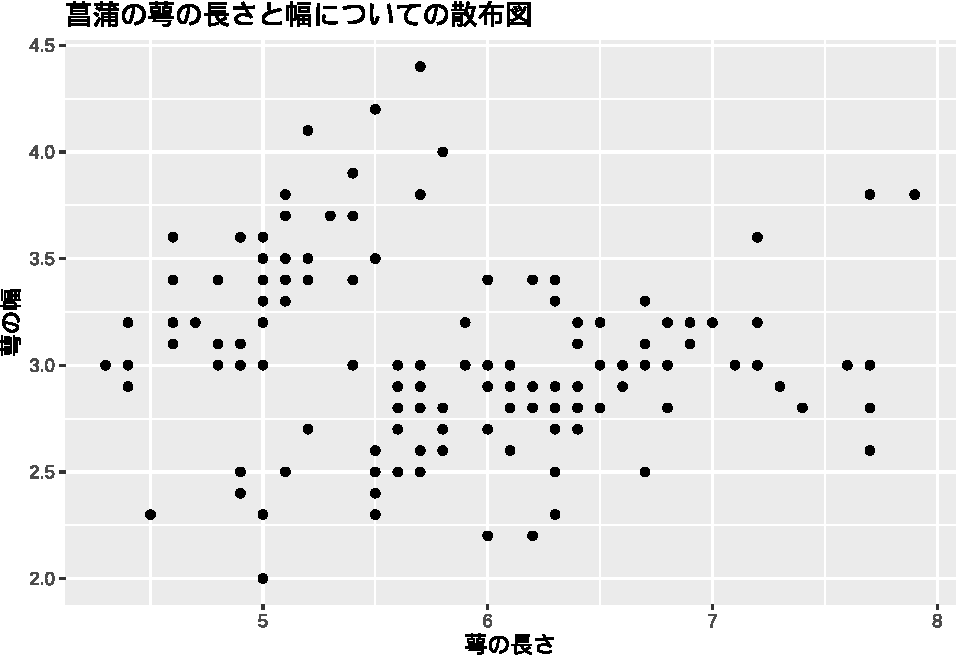
\includegraphics{31-worldbank_files/figure-latex/unnamed-chunk-8-1.pdf}

\begin{Shaded}
\begin{Highlighting}[]
\FunctionTok{WDI}\NormalTok{(}\AttributeTok{country =} \FunctionTok{c}\NormalTok{(}\StringTok{"CN"}\NormalTok{,}\StringTok{"IN"}\NormalTok{,}\StringTok{"JP"}\NormalTok{,}\StringTok{"US"}\NormalTok{), }
    \AttributeTok{indicator =} \FunctionTok{c}\NormalTok{(}\AttributeTok{gdp\_growth\_rate =} \StringTok{"NY.GDP.MKTP.KD.ZG"}\NormalTok{), }\AttributeTok{extra=}\ConstantTok{TRUE}\NormalTok{) }\SpecialCharTok{\%\textgreater{}\%}
  \FunctionTok{drop\_na}\NormalTok{(gdp\_growth\_rate) }\SpecialCharTok{\%\textgreater{}\%} 
  \FunctionTok{ggplot}\NormalTok{(}\FunctionTok{aes}\NormalTok{(year, gdp\_growth\_rate, }\AttributeTok{col =}\NormalTok{ country)) }\SpecialCharTok{+} \FunctionTok{geom\_line}\NormalTok{() }\SpecialCharTok{+}
  \FunctionTok{labs}\NormalTok{(}\AttributeTok{title =} \FunctionTok{paste}\NormalTok{(}\StringTok{"WDI NY.GDP.MKTP.KD.ZG: gdp growth rate"}\NormalTok{))}
\end{Highlighting}
\end{Shaded}

\begin{verbatim}
#> Rows: 248 Columns: 13
#> -- Column specification ------------------------------------
#> Delimiter: ","
#> chr  (7): country, iso2c, iso3c, region, capital, income...
#> dbl  (4): year, gdp_growth_rate, longitude, latitude
#> lgl  (1): status
#> date (1): lastupdated
#> 
#> i Use `spec()` to retrieve the full column specification for this data.
#> i Specify the column types or set `show_col_types = FALSE` to quiet this message.
\end{verbatim}

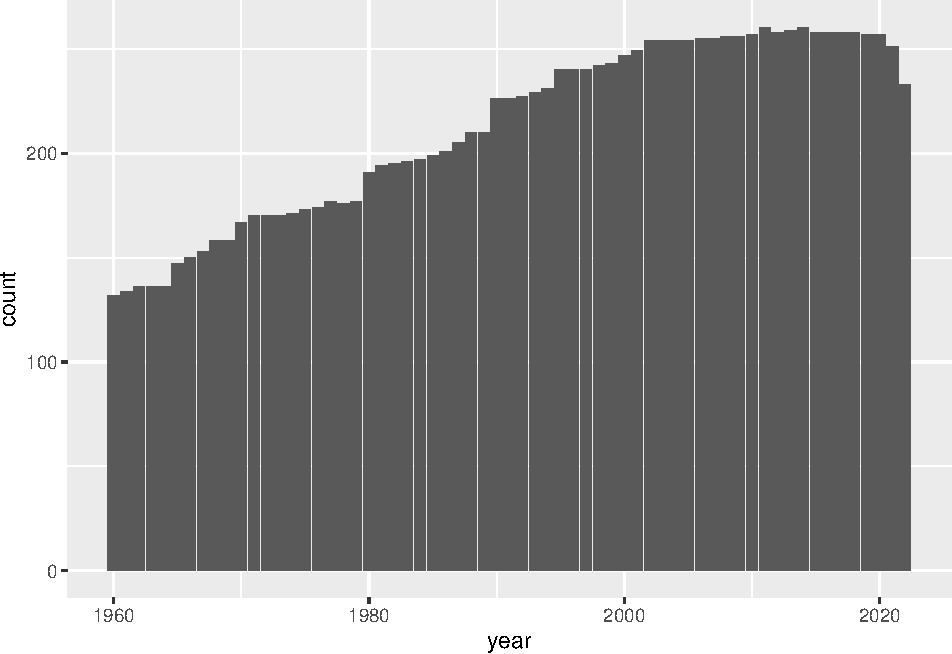
\includegraphics{31-worldbank_files/figure-latex/unnamed-chunk-11-1.pdf}

まず、世界の国々の、GDP(gross domestic product 国内総生産)のデータを、取得して、2021年の GDP を大きな順に並べています。

値は、たとえば、\(2.331508e+13\) のように書かれていますが、これは、科学的記法と呼ばれるもので、\(2.331508 \times 10^{13}\) を意味しています。約23兆ドルです。

次に、3兆ドル以上の、6カ国を選択し、その、iso2c と呼ばれるコードを使って、それらの国のデータをもう一度取得し、年次変化をあらわすグラフを描いています。

さらにその中から、4カ国を選んで、今度は、GDP の年次変化率を描いています。単位は、パーセントです。

これは、ひとつの例ですが、ここで使われているのが、WDI World Development Indicator というもので、世界銀行が、いくつかの指標を定めて、編纂しているものです。

\hypertarget{ux6307ux6a19-indicators-wdi}{%
\subsubsection{指標 Indicators (WDI)}\label{ux6307ux6a19-indicators-wdi}}

上の例では、次の二つの指標のコード Indicator Code (WDI Code) が使われました。

\begin{itemize}
\tightlist
\item
  NY.GDP.MKTP.CD: GDP (current US\$)
\item
  NY.GDP.MKTP.KD.ZG: GDP growth (annual \%)
\end{itemize}

\hypertarget{ux6307ux6a19-wdi-world-development-indicators}{%
\subsubsection{指標 WDI (World Development Indicators)}\label{ux6307ux6a19-wdi-world-development-indicators}}

\begin{quote}
The World Development Indicators is a compilation of relevant, high-quality, and internationally comparable statistics about global development and the fight against poverty. The database contains 1,400 time series indicators for 217 economies and more than 40 country groups, with data for many indicators going back more than 50 years.
\end{quote}

\begin{quote}
WDIは、世界の開発状況と、貧困との戦いに関する、適切で上質、かつ、国際的に比較可能な時系列の統計データを編纂したものです。このデータベースは、217の経済と40以上の国グループについて1,400の時系列指標を含み、指標のデータの多くは50年以上前に遡ることができます。
\end{quote}

\begin{itemize}
\tightlist
\item
  世界銀行(World Bank): \url{https://www.worldbank.org}
\item
  World Bank Open Data: \url{https://data.worldbank.org}

  \begin{itemize}
  \tightlist
  \item
    Country / Indicator \textgreater{} Featured \& All \textgreater{} Details
  \end{itemize}
\item
  \href{https://datatopics.worldbank.org/world-development-indicators/}{World Development Indicators (WDI)} :

  \begin{itemize}
  \tightlist
  \item
    Themes: Poverty and Inequality, People, Environment, Economy, States and Markets, Global Links
  \item
    Open Data \& DataBank: Explore data, Query database
  \end{itemize}
\end{itemize}

\hypertarget{ux6307ux6a19-ux306eux30b3ux30fcux30c9wdi-code-ux3092ux63a2ux3057ux3066ux307fux3088ux3046}{%
\subsubsection{指標 のコード、WDI code を探してみよう}\label{ux6307ux6a19-ux306eux30b3ux30fcux30c9wdi-code-ux3092ux63a2ux3057ux3066ux307fux3088ux3046}}

いくつかの探し方があります。まず、ここでは、World Bank のサイトから探す方法を説明しましょう。

ふた通りあります。

\begin{enumerate}
\def\labelenumi{\arabic{enumi}.}
\item
  \href{https://data.worldbank.org}{World Bank Open Data} にいくと、表題の下の検索窓の下に、 Country / Indicator とありますから、Indicator を選択します。すると、そこに、項目のリストが、Featured と All という二つのタブに分かれて出ています。かなり膨大です。それを選択すると、その項目のサイトに行きます。それが、指標のサイトです。図などの、右上に、Details とありますから、それを選択すると、その中に、Indicator が書かれています。
  実は、指標のサイトのアドレス(URL)を見ると、そこにも、この Indicator が書かれていることがわかります。
\item
  \href{https://datatopics.worldbank.org/world-development-indicators/}{World Development Indicators (WDI)} にいくと、下のようなテーマに分かれています。
\end{enumerate}

Themes: Poverty and Inequality, People, Environment, Economy, States and Markets, Global Links

その中から、選択して、スクロールすると、そこに、指標が書かれています。

Indicator, Code, Time coverage, Region coverage, Get data

とあり、Code が、指標のコードです。実は、すべての年や、すべての地域のデータが揃っているわけではないので、この情報を見ておくことはとても重要です。ほとんど、データがない場合もあります。

一番右端の Get data からは、CSV や、データバンク(Data Bank)へのリンクがあります。

それぞれの方法で、上で使った、二つの指標およびそのコードは見つかりましたか。

1 の方法の途中に出てきた、検索窓から検索することも可能です。

\hypertarget{ux6307ux6a19-wdiux306eux4f8b}{%
\subsubsection{指標 WDIの例}\label{ux6307ux6a19-wdiux306eux4f8b}}

このあとの、例で使う指標を書いておきます。

\begin{itemize}
\tightlist
\item
  NY.GDP.MKTP.CD: GDP (current US\$)
\item
  NY.GDP.DEFL.KD.ZG: Inflation, GDP deflator (annual \%)
\item
  SL.UEM.TOTL.NE.ZS: Unemployment, total (\% of total labor force) (national estimate)
\item
  CPTOTNSXN: CPI Price, nominal
\item
  SL.TLF.CACT.MA.NE.ZS: Labor force participation rate, male (\% of male population ages 15+) (national estimate)
\item
  SL.TLF.CACT.FE.NE.ZS: Labor force participation rate, female (\% of male population ages 15+) (national estimate)
\end{itemize}

\hypertarget{ux7df4ux7fd2-1.---ux8abfux3079ux3066ux307fux305fux3044-wdi-ux6307ux6a19ux3068ux305dux306eux30b3ux30fcux30c9}{%
\subsubsection{練習 1. - 調べてみたい WDI 指標とそのコード}\label{ux7df4ux7fd2-1.---ux8abfux3079ux3066ux307fux305fux3044-wdi-ux6307ux6a19ux3068ux305dux306eux30b3ux30fcux30c9}}

いくつか、リストしてみましょう。

\hypertarget{wdi-ux30d1ux30c3ux30b1ux30fcux30b8}{%
\subsection{WDI パッケージ}\label{wdi-ux30d1ux30c3ux30b1ux30fcux30b8}}

\texttt{WDI} パッケージ の使い方を紹介します。

\texttt{WDI} パッケージで、データをダウンロードしたり、探したり、詳細情報を得たりできます。

\hypertarget{ux6307ux6a19-wdi-ux691cux7d22}{%
\subsubsection{指標 WDI 検索}\label{ux6307ux6a19-wdi-ux691cux7d22}}

まず、検索です。上で、サイトから調べる方法を紹介しましたが、\texttt{WDI} パッケージの、\texttt{WDIsearch} でも探すことができます。詳細は、右下の窓枠の Help タブの検索窓に、WDIsearch といれて調べて見てください。ここでは、二種類の検索方法を紹介します。

\hypertarget{ux691cux7d22ux4f8b-1wdiux540d}{%
\paragraph{検索例 1(WDI名)}\label{ux691cux7d22ux4f8b-1wdiux540d}}

WDI 名に、ある文字列が含まれているものを検索します。検索文字列は、大文字・小文字は関係ありません。

\begin{Shaded}
\begin{Highlighting}[]
\FunctionTok{WDIsearch}\NormalTok{(}\AttributeTok{string =} \StringTok{"gdp"}\NormalTok{, }\AttributeTok{field =} \StringTok{"name"}\NormalTok{, }\AttributeTok{short =} \ConstantTok{TRUE}\NormalTok{, }\AttributeTok{cache =} \ConstantTok{NULL}\NormalTok{)}
\CommentTok{\#\textgreater{}                        indicator}
\CommentTok{\#\textgreater{} 712               5.51.01.10.gdp}
\CommentTok{\#\textgreater{} 714              6.0.GDP\_current}
\CommentTok{\#\textgreater{} 715               6.0.GDP\_growth}
\CommentTok{\#\textgreater{} 716                  6.0.GDP\_usd}
\CommentTok{\#\textgreater{} 717           6.0.GDPpc\_constant}
\CommentTok{\#\textgreater{} 1557           BG.GSR.NFSV.GD.ZS}
\CommentTok{\#\textgreater{} 1558        BG.KAC.FNEI.GD.PP.ZS}
\CommentTok{\#\textgreater{} 1559           BG.KAC.FNEI.GD.ZS}
\CommentTok{\#\textgreater{} 1560        BG.KLT.DINV.GD.PP.ZS}
\CommentTok{\#\textgreater{} 1561           BG.KLT.DINV.GD.ZS}
\CommentTok{\#\textgreater{} 1752           BI.WAG.TOTL.GD.ZS}
\CommentTok{\#\textgreater{} 1772              BM.GSR.MRCH.ZS}
\CommentTok{\#\textgreater{} 1784           BM.KLT.DINV.GD.ZS}
\CommentTok{\#\textgreater{} 1785        BM.KLT.DINV.WD.GD.ZS}
\CommentTok{\#\textgreater{} 1798           BN.CAB.XOKA.GD.ZS}
\CommentTok{\#\textgreater{} 1799          BN.CAB.XOKA.GDP.ZS}
\CommentTok{\#\textgreater{} 1802              BN.CAB.XOTR.ZS}
\CommentTok{\#\textgreater{} 1805              BN.CUR.GDPM.ZS}
\CommentTok{\#\textgreater{} 1811           BN.GSR.FCTY.CD.ZS}
\CommentTok{\#\textgreater{} 1820           BN.KLT.DINV.CD.ZS}
\CommentTok{\#\textgreater{} 1822      BN.KLT.DINV.DRS.GDP.ZS}
\CommentTok{\#\textgreater{} 1828           BN.KLT.PRVT.GD.ZS}
\CommentTok{\#\textgreater{} 1839           BN.TRF.CURR.CD.ZS}
\CommentTok{\#\textgreater{} 1875              BX.GSR.MRCH.ZS}
\CommentTok{\#\textgreater{} 1887        BX.KLT.DINV.DT.GD.ZS}
\CommentTok{\#\textgreater{} 1889        BX.KLT.DINV.WD.GD.ZS}
\CommentTok{\#\textgreater{} 1898         BX.TRF.MGR.DT.GD.ZS}
\CommentTok{\#\textgreater{} 1904        BX.TRF.PWKR.DT.GD.ZS}
\CommentTok{\#\textgreater{} 1905           BX.TRF.PWKR.GD.ZS}
\CommentTok{\#\textgreater{} 2198              CC.ENTX.ENE.ZS}
\CommentTok{\#\textgreater{} 2270              CC.GHG.MEMG.EI}
\CommentTok{\#\textgreater{} 2271              CC.GHG.MEMG.GC}
\CommentTok{\#\textgreater{} 2293                CC.INCP.ALRS}
\CommentTok{\#\textgreater{} 2294                CC.INCP.KRGC}
\CommentTok{\#\textgreater{} 2295                CC.INCP.SPMC}
\CommentTok{\#\textgreater{} 2356              CC.RISK.AST.ZS}
\CommentTok{\#\textgreater{} 2357             CC.RISK.WELL.ZS}
\CommentTok{\#\textgreater{} 2364                CC.SP.EXP.ZS}
\CommentTok{\#\textgreater{} 2401           CM.FIN.INTL.GD.ZS}
\CommentTok{\#\textgreater{} 2404           CM.MKT.LCAP.GD.ZS}
\CommentTok{\#\textgreater{} 2407           CM.MKT.TRAD.GD.ZS}
\CommentTok{\#\textgreater{} 2559        DP.DOD.DECD.CR.BC.Z1}
\CommentTok{\#\textgreater{} 2562        DP.DOD.DECD.CR.CG.Z1}
\CommentTok{\#\textgreater{} 2565        DP.DOD.DECD.CR.FC.Z1}
\CommentTok{\#\textgreater{} 2568        DP.DOD.DECD.CR.GG.Z1}
\CommentTok{\#\textgreater{} 2571        DP.DOD.DECD.CR.NF.Z1}
\CommentTok{\#\textgreater{} 2576        DP.DOD.DECF.CR.BC.Z1}
\CommentTok{\#\textgreater{} 2579        DP.DOD.DECF.CR.CG.Z1}
\CommentTok{\#\textgreater{} 2582        DP.DOD.DECF.CR.FC.Z1}
\CommentTok{\#\textgreater{} 2585        DP.DOD.DECF.CR.GG.Z1}
\CommentTok{\#\textgreater{} 2588        DP.DOD.DECF.CR.NF.Z1}
\CommentTok{\#\textgreater{} 2593        DP.DOD.DECN.CR.BC.Z1}
\CommentTok{\#\textgreater{} 2596        DP.DOD.DECN.CR.CG.Z1}
\CommentTok{\#\textgreater{} 2599        DP.DOD.DECN.CR.FC.Z1}
\CommentTok{\#\textgreater{} 2602        DP.DOD.DECN.CR.GG.Z1}
\CommentTok{\#\textgreater{} 2605        DP.DOD.DECN.CR.NF.Z1}
\CommentTok{\#\textgreater{} 2610        DP.DOD.DECT.CR.BC.Z1}
\CommentTok{\#\textgreater{} 2613        DP.DOD.DECT.CR.CG.Z1}
\CommentTok{\#\textgreater{} 2616        DP.DOD.DECT.CR.FC.Z1}
\CommentTok{\#\textgreater{} 2619        DP.DOD.DECT.CR.GG.Z1}
\CommentTok{\#\textgreater{} 2622        DP.DOD.DECT.CR.NF.Z1}
\CommentTok{\#\textgreater{} 2627        DP.DOD.DECX.CR.BC.Z1}
\CommentTok{\#\textgreater{} 2630        DP.DOD.DECX.CR.CG.Z1}
\CommentTok{\#\textgreater{} 2633        DP.DOD.DECX.CR.FC.Z1}
\CommentTok{\#\textgreater{} 2636        DP.DOD.DECX.CR.GG.Z1}
\CommentTok{\#\textgreater{} 2639        DP.DOD.DECX.CR.NF.Z1}
\CommentTok{\#\textgreater{} 2644        DP.DOD.DLCD.CR.BC.Z1}
\CommentTok{\#\textgreater{} 2647        DP.DOD.DLCD.CR.CG.Z1}
\CommentTok{\#\textgreater{} 2650        DP.DOD.DLCD.CR.FC.Z1}
\CommentTok{\#\textgreater{} 2653        DP.DOD.DLCD.CR.GG.Z1}
\CommentTok{\#\textgreater{} 2656     DP.DOD.DLCD.CR.L1.BC.Z1}
\CommentTok{\#\textgreater{} 2659     DP.DOD.DLCD.CR.L1.CG.Z1}
\CommentTok{\#\textgreater{} 2662     DP.DOD.DLCD.CR.L1.FC.Z1}
\CommentTok{\#\textgreater{} 2665     DP.DOD.DLCD.CR.L1.GG.Z1}
\CommentTok{\#\textgreater{} 2668     DP.DOD.DLCD.CR.L1.NF.Z1}
\CommentTok{\#\textgreater{} 2673     DP.DOD.DLCD.CR.M1.BC.Z1}
\CommentTok{\#\textgreater{} 2676     DP.DOD.DLCD.CR.M1.CG.Z1}
\CommentTok{\#\textgreater{} 2679     DP.DOD.DLCD.CR.M1.FC.Z1}
\CommentTok{\#\textgreater{} 2682     DP.DOD.DLCD.CR.M1.GG.Z1}
\CommentTok{\#\textgreater{} 2685     DP.DOD.DLCD.CR.M1.NF.Z1}
\CommentTok{\#\textgreater{} 2690        DP.DOD.DLCD.CR.NF.Z1}
\CommentTok{\#\textgreater{} 2694        DP.DOD.DLD1.CR.CG.Z1}
\CommentTok{\#\textgreater{} 2696        DP.DOD.DLD1.CR.GG.Z1}
\CommentTok{\#\textgreater{} 2698        DP.DOD.DLD2.CR.CG.Z1}
\CommentTok{\#\textgreater{} 2700        DP.DOD.DLD2.CR.GG.Z1}
\CommentTok{\#\textgreater{} 2702       DP.DOD.DLD2A.CR.CG.Z1}
\CommentTok{\#\textgreater{} 2704       DP.DOD.DLD2A.CR.GG.Z1}
\CommentTok{\#\textgreater{} 2706        DP.DOD.DLD3.CR.CG.Z1}
\CommentTok{\#\textgreater{} 2708        DP.DOD.DLD3.CR.GG.Z1}
\CommentTok{\#\textgreater{} 2710        DP.DOD.DLD4.CR.CG.Z1}
\CommentTok{\#\textgreater{} 2712        DP.DOD.DLD4.CR.GG.Z1}
\CommentTok{\#\textgreater{} 2715        DP.DOD.DLDS.CR.BC.Z1}
\CommentTok{\#\textgreater{} 2718        DP.DOD.DLDS.CR.CG.Z1}
\CommentTok{\#\textgreater{} 2721        DP.DOD.DLDS.CR.FC.Z1}
\CommentTok{\#\textgreater{} 2724        DP.DOD.DLDS.CR.GG.Z1}
\CommentTok{\#\textgreater{} 2727     DP.DOD.DLDS.CR.L1.BC.Z1}
\CommentTok{\#\textgreater{} 2730     DP.DOD.DLDS.CR.L1.CG.Z1}
\CommentTok{\#\textgreater{} 2733     DP.DOD.DLDS.CR.L1.FC.Z1}
\CommentTok{\#\textgreater{} 2736     DP.DOD.DLDS.CR.L1.GG.Z1}
\CommentTok{\#\textgreater{} 2739     DP.DOD.DLDS.CR.L1.NF.Z1}
\CommentTok{\#\textgreater{} 2744     DP.DOD.DLDS.CR.M1.BC.Z1}
\CommentTok{\#\textgreater{} 2747     DP.DOD.DLDS.CR.M1.CG.Z1}
\CommentTok{\#\textgreater{} 2750     DP.DOD.DLDS.CR.M1.FC.Z1}
\CommentTok{\#\textgreater{} 2753     DP.DOD.DLDS.CR.M1.GG.Z1}
\CommentTok{\#\textgreater{} 2756     DP.DOD.DLDS.CR.M1.NF.Z1}
\CommentTok{\#\textgreater{} 2761     DP.DOD.DLDS.CR.MV.BC.Z1}
\CommentTok{\#\textgreater{} 2764     DP.DOD.DLDS.CR.MV.CG.Z1}
\CommentTok{\#\textgreater{} 2767     DP.DOD.DLDS.CR.MV.FC.Z1}
\CommentTok{\#\textgreater{} 2770     DP.DOD.DLDS.CR.MV.GG.Z1}
\CommentTok{\#\textgreater{} 2773     DP.DOD.DLDS.CR.MV.NF.Z1}
\CommentTok{\#\textgreater{} 2778        DP.DOD.DLDS.CR.NF.Z1}
\CommentTok{\#\textgreater{} 2783        DP.DOD.DLIN.CR.BC.Z1}
\CommentTok{\#\textgreater{} 2786        DP.DOD.DLIN.CR.CG.Z1}
\CommentTok{\#\textgreater{} 2789        DP.DOD.DLIN.CR.FC.Z1}
\CommentTok{\#\textgreater{} 2792        DP.DOD.DLIN.CR.GG.Z1}
\CommentTok{\#\textgreater{} 2795     DP.DOD.DLIN.CR.L1.BC.Z1}
\CommentTok{\#\textgreater{} 2798     DP.DOD.DLIN.CR.L1.CG.Z1}
\CommentTok{\#\textgreater{} 2801     DP.DOD.DLIN.CR.L1.FC.Z1}
\CommentTok{\#\textgreater{} 2804     DP.DOD.DLIN.CR.L1.GG.Z1}
\CommentTok{\#\textgreater{} 2807     DP.DOD.DLIN.CR.L1.NF.Z1}
\CommentTok{\#\textgreater{} 2812     DP.DOD.DLIN.CR.M1.BC.Z1}
\CommentTok{\#\textgreater{} 2815     DP.DOD.DLIN.CR.M1.CG.Z1}
\CommentTok{\#\textgreater{} 2818     DP.DOD.DLIN.CR.M1.FC.Z1}
\CommentTok{\#\textgreater{} 2821     DP.DOD.DLIN.CR.M1.GG.Z1}
\CommentTok{\#\textgreater{} 2824     DP.DOD.DLIN.CR.M1.NF.Z1}
\CommentTok{\#\textgreater{} 2829        DP.DOD.DLIN.CR.NF.Z1}
\CommentTok{\#\textgreater{} 2834        DP.DOD.DLLO.CR.BC.Z1}
\CommentTok{\#\textgreater{} 2837        DP.DOD.DLLO.CR.CG.Z1}
\CommentTok{\#\textgreater{} 2840        DP.DOD.DLLO.CR.FC.Z1}
\CommentTok{\#\textgreater{} 2843        DP.DOD.DLLO.CR.GG.Z1}
\CommentTok{\#\textgreater{} 2846     DP.DOD.DLLO.CR.L1.BC.Z1}
\CommentTok{\#\textgreater{} 2849     DP.DOD.DLLO.CR.L1.CG.Z1}
\CommentTok{\#\textgreater{} 2852     DP.DOD.DLLO.CR.L1.FC.Z1}
\CommentTok{\#\textgreater{} 2855     DP.DOD.DLLO.CR.L1.GG.Z1}
\CommentTok{\#\textgreater{} 2858     DP.DOD.DLLO.CR.L1.NF.Z1}
\CommentTok{\#\textgreater{} 2863     DP.DOD.DLLO.CR.M1.BC.Z1}
\CommentTok{\#\textgreater{} 2866     DP.DOD.DLLO.CR.M1.CG.Z1}
\CommentTok{\#\textgreater{} 2869     DP.DOD.DLLO.CR.M1.FC.Z1}
\CommentTok{\#\textgreater{} 2872     DP.DOD.DLLO.CR.M1.GG.Z1}
\CommentTok{\#\textgreater{} 2875     DP.DOD.DLLO.CR.M1.NF.Z1}
\CommentTok{\#\textgreater{} 2880        DP.DOD.DLLO.CR.NF.Z1}
\CommentTok{\#\textgreater{} 2885        DP.DOD.DLOA.CR.BC.Z1}
\CommentTok{\#\textgreater{} 2888        DP.DOD.DLOA.CR.CG.Z1}
\CommentTok{\#\textgreater{} 2891        DP.DOD.DLOA.CR.FC.Z1}
\CommentTok{\#\textgreater{} 2894        DP.DOD.DLOA.CR.GG.Z1}
\CommentTok{\#\textgreater{} 2897     DP.DOD.DLOA.CR.L1.BC.Z1}
\CommentTok{\#\textgreater{} 2900     DP.DOD.DLOA.CR.L1.CG.Z1}
\CommentTok{\#\textgreater{} 2903     DP.DOD.DLOA.CR.L1.FC.Z1}
\CommentTok{\#\textgreater{} 2906     DP.DOD.DLOA.CR.L1.GG.Z1}
\CommentTok{\#\textgreater{} 2909     DP.DOD.DLOA.CR.L1.NF.Z1}
\CommentTok{\#\textgreater{} 2914     DP.DOD.DLOA.CR.M1.BC.Z1}
\CommentTok{\#\textgreater{} 2917     DP.DOD.DLOA.CR.M1.CG.Z1}
\CommentTok{\#\textgreater{} 2920     DP.DOD.DLOA.CR.M1.FC.Z1}
\CommentTok{\#\textgreater{} 2923     DP.DOD.DLOA.CR.M1.GG.Z1}
\CommentTok{\#\textgreater{} 2926     DP.DOD.DLOA.CR.M1.NF.Z1}
\CommentTok{\#\textgreater{} 2931        DP.DOD.DLOA.CR.NF.Z1}
\CommentTok{\#\textgreater{} 2936        DP.DOD.DLSD.CR.BC.Z1}
\CommentTok{\#\textgreater{} 2939        DP.DOD.DLSD.CR.CG.Z1}
\CommentTok{\#\textgreater{} 2942        DP.DOD.DLSD.CR.FC.Z1}
\CommentTok{\#\textgreater{} 2945        DP.DOD.DLSD.CR.GG.Z1}
\CommentTok{\#\textgreater{} 2948     DP.DOD.DLSD.CR.M1.BC.Z1}
\CommentTok{\#\textgreater{} 2951     DP.DOD.DLSD.CR.M1.CG.Z1}
\CommentTok{\#\textgreater{} 2954     DP.DOD.DLSD.CR.M1.FC.Z1}
\CommentTok{\#\textgreater{} 2957     DP.DOD.DLSD.CR.M1.GG.Z1}
\CommentTok{\#\textgreater{} 2960     DP.DOD.DLSD.CR.M1.NF.Z1}
\CommentTok{\#\textgreater{} 2965        DP.DOD.DLSD.CR.NF.Z1}
\CommentTok{\#\textgreater{} 2970        DP.DOD.DLTC.CR.BC.Z1}
\CommentTok{\#\textgreater{} 2973        DP.DOD.DLTC.CR.CG.Z1}
\CommentTok{\#\textgreater{} 2976        DP.DOD.DLTC.CR.FC.Z1}
\CommentTok{\#\textgreater{} 2979        DP.DOD.DLTC.CR.GG.Z1}
\CommentTok{\#\textgreater{} 2982     DP.DOD.DLTC.CR.L1.BC.Z1}
\CommentTok{\#\textgreater{} 2985     DP.DOD.DLTC.CR.L1.CG.Z1}
\CommentTok{\#\textgreater{} 2988     DP.DOD.DLTC.CR.L1.FC.Z1}
\CommentTok{\#\textgreater{} 2991     DP.DOD.DLTC.CR.L1.GG.Z1}
\CommentTok{\#\textgreater{} 2994     DP.DOD.DLTC.CR.L1.NF.Z1}
\CommentTok{\#\textgreater{} 2999     DP.DOD.DLTC.CR.M1.BC.Z1}
\CommentTok{\#\textgreater{} 3002     DP.DOD.DLTC.CR.M1.CG.Z1}
\CommentTok{\#\textgreater{} 3005     DP.DOD.DLTC.CR.M1.FC.Z1}
\CommentTok{\#\textgreater{} 3008     DP.DOD.DLTC.CR.M1.GG.Z1}
\CommentTok{\#\textgreater{} 3011     DP.DOD.DLTC.CR.M1.NF.Z1}
\CommentTok{\#\textgreater{} 3016        DP.DOD.DLTC.CR.NF.Z1}
\CommentTok{\#\textgreater{} 3022        DP.DOD.DSCD.CR.BC.Z1}
\CommentTok{\#\textgreater{} 3025        DP.DOD.DSCD.CR.CG.Z1}
\CommentTok{\#\textgreater{} 3028        DP.DOD.DSCD.CR.FC.Z1}
\CommentTok{\#\textgreater{} 3031        DP.DOD.DSCD.CR.GG.Z1}
\CommentTok{\#\textgreater{} 3034        DP.DOD.DSCD.CR.NF.Z1}
\CommentTok{\#\textgreater{} 3039        DP.DOD.DSDS.CR.BC.Z1}
\CommentTok{\#\textgreater{} 3042        DP.DOD.DSDS.CR.CG.Z1}
\CommentTok{\#\textgreater{} 3045        DP.DOD.DSDS.CR.FC.Z1}
\CommentTok{\#\textgreater{} 3048        DP.DOD.DSDS.CR.GG.Z1}
\CommentTok{\#\textgreater{} 3051        DP.DOD.DSDS.CR.NF.Z1}
\CommentTok{\#\textgreater{} 3056        DP.DOD.DSIN.CR.BC.Z1}
\CommentTok{\#\textgreater{} 3059        DP.DOD.DSIN.CR.CG.Z1}
\CommentTok{\#\textgreater{} 3062        DP.DOD.DSIN.CR.FC.Z1}
\CommentTok{\#\textgreater{} 3065        DP.DOD.DSIN.CR.GG.Z1}
\CommentTok{\#\textgreater{} 3068        DP.DOD.DSIN.CR.NF.Z1}
\CommentTok{\#\textgreater{} 3073        DP.DOD.DSLO.CR.BC.Z1}
\CommentTok{\#\textgreater{} 3076        DP.DOD.DSLO.CR.CG.Z1}
\CommentTok{\#\textgreater{} 3079        DP.DOD.DSLO.CR.FC.Z1}
\CommentTok{\#\textgreater{} 3082        DP.DOD.DSLO.CR.GG.Z1}
\CommentTok{\#\textgreater{} 3085        DP.DOD.DSLO.CR.NF.Z1}
\CommentTok{\#\textgreater{} 3090        DP.DOD.DSOA.CR.BC.Z1}
\CommentTok{\#\textgreater{} 3093        DP.DOD.DSOA.CR.CG.Z1}
\CommentTok{\#\textgreater{} 3096        DP.DOD.DSOA.CR.FC.Z1}
\CommentTok{\#\textgreater{} 3099        DP.DOD.DSOA.CR.GG.Z1}
\CommentTok{\#\textgreater{} 3102        DP.DOD.DSOA.CR.NF.Z1}
\CommentTok{\#\textgreater{} 3107        DP.DOD.DSTC.CR.BC.Z1}
\CommentTok{\#\textgreater{} 3110        DP.DOD.DSTC.CR.CG.Z1}
\CommentTok{\#\textgreater{} 3113        DP.DOD.DSTC.CR.FC.Z1}
\CommentTok{\#\textgreater{} 3116        DP.DOD.DSTC.CR.GG.Z1}
\CommentTok{\#\textgreater{} 3119        DP.DOD.DSTC.CR.NF.Z1}
\CommentTok{\#\textgreater{} 3615             DT.DOD.ALLC.ZSG}
\CommentTok{\#\textgreater{} 3618             DT.DOD.ALLN.ZSG}
\CommentTok{\#\textgreater{} 3773          DT.DOD.DECT.CD.ZSG}
\CommentTok{\#\textgreater{} 5376           DT.ODA.ALLD.GD.ZS}
\CommentTok{\#\textgreater{} 5447             DT.ODA.DACD.ZSG}
\CommentTok{\#\textgreater{} 5452             DT.ODA.MULT.ZSG}
\CommentTok{\#\textgreater{} 5460             DT.ODA.NDAC.ZSG}
\CommentTok{\#\textgreater{} 5466           DT.ODA.ODAT.GD.ZS}
\CommentTok{\#\textgreater{} 5616           DT.TDS.DECT.GD.ZS}
\CommentTok{\#\textgreater{} 5969           EG.EGY.PRIM.PP.KD}
\CommentTok{\#\textgreater{} 5993           EG.GDP.PUSE.KO.87}
\CommentTok{\#\textgreater{} 5994           EG.GDP.PUSE.KO.KD}
\CommentTok{\#\textgreater{} 5995           EG.GDP.PUSE.KO.PP}
\CommentTok{\#\textgreater{} 5996        EG.GDP.PUSE.KO.PP.KD}
\CommentTok{\#\textgreater{} 6004        EG.USE.COMM.GD.PP.KD}
\CommentTok{\#\textgreater{} 6023             EN.ATM.CO2E.GDP}
\CommentTok{\#\textgreater{} 6027        EN.ATM.CO2E.KD.87.GD}
\CommentTok{\#\textgreater{} 6028           EN.ATM.CO2E.KD.GD}
\CommentTok{\#\textgreater{} 6033           EN.ATM.CO2E.PP.GD}
\CommentTok{\#\textgreater{} 6034        EN.ATM.CO2E.PP.GD.KD}
\CommentTok{\#\textgreater{} 6164           ER.GDP.FWTL.M3.KD}
\CommentTok{\#\textgreater{} 6182             EU.EGY.USES.GDP}
\CommentTok{\#\textgreater{} 6236           FB.DPT.INSU.PC.ZS}
\CommentTok{\#\textgreater{} 6589           FD.AST.PRVT.GD.ZS}
\CommentTok{\#\textgreater{} 6595           FI.RES.TOTL.CD.ZS}
\CommentTok{\#\textgreater{} 7389           FM.AST.GOVT.CN.ZS}
\CommentTok{\#\textgreater{} 7398           FM.AST.PRVT.GD.ZS}
\CommentTok{\#\textgreater{} 7407           FM.LBL.BMNY.GD.ZS}
\CommentTok{\#\textgreater{} 7414           FM.LBL.MQMY.GD.ZS}
\CommentTok{\#\textgreater{} 7415          FM.LBL.MQMY.GDP.ZS}
\CommentTok{\#\textgreater{} 7417              FM.LBL.MQMY.XD}
\CommentTok{\#\textgreater{} 7422          FM.LBL.QMNY.GDP.ZS}
\CommentTok{\#\textgreater{} 7423          FM.LBL.SEIG.GDP.ZS}
\CommentTok{\#\textgreater{} 7462           FS.AST.CGOV.GD.ZS}
\CommentTok{\#\textgreater{} 7463           FS.AST.DOMO.GD.ZS}
\CommentTok{\#\textgreater{} 7464           FS.AST.DOMS.GD.ZS}
\CommentTok{\#\textgreater{} 7465              FS.AST.DTOT.ZS}
\CommentTok{\#\textgreater{} 7467           FS.AST.PRVT.GD.ZS}
\CommentTok{\#\textgreater{} 7468          FS.AST.PRVT.GDP.ZS}
\CommentTok{\#\textgreater{} 7469           FS.LBL.LIQU.GD.ZS}
\CommentTok{\#\textgreater{} 7470          FS.LBL.LIQU.GDP.ZS}
\CommentTok{\#\textgreater{} 7471           FS.LBL.QLIQ.GD.ZS}
\CommentTok{\#\textgreater{} 7530           GB.BAL.OVRL.GD.ZS}
\CommentTok{\#\textgreater{} 7531          GB.BAL.OVRL.GDP.ZS}
\CommentTok{\#\textgreater{} 7540           GB.DOD.TOTL.GD.ZS}
\CommentTok{\#\textgreater{} 7541          GB.DOD.TOTL.GDP.ZS}
\CommentTok{\#\textgreater{} 7545           GB.FIN.ABRD.GD.ZS}
\CommentTok{\#\textgreater{} 7546          GB.FIN.ABRD.GDP.ZS}
\CommentTok{\#\textgreater{} 7550           GB.FIN.DOMS.GD.ZS}
\CommentTok{\#\textgreater{} 7551          GB.FIN.DOMS.GDP.ZS}
\CommentTok{\#\textgreater{} 7561           GB.REV.CTOT.GD.ZS}
\CommentTok{\#\textgreater{} 7564          GB.REV.TOTL.GDP.ZS}
\CommentTok{\#\textgreater{} 7566           GB.REV.XAGT.CN.ZS}
\CommentTok{\#\textgreater{} 7569           GB.RVC.TOTL.GD.ZS}
\CommentTok{\#\textgreater{} 7571              GB.SOE.DECT.ZS}
\CommentTok{\#\textgreater{} 7573           GB.SOE.ECON.GD.ZS}
\CommentTok{\#\textgreater{} 7574          GB.SOE.ECON.GDP.ZS}
\CommentTok{\#\textgreater{} 7577           GB.SOE.NFLW.GD.ZS}
\CommentTok{\#\textgreater{} 7578          GB.SOE.NFLW.GDP.ZS}
\CommentTok{\#\textgreater{} 7579           GB.SOE.OVRL.GD.ZS}
\CommentTok{\#\textgreater{} 7605           GB.TAX.TOTL.GD.ZS}
\CommentTok{\#\textgreater{} 7606          GB.TAX.TOTL.GDP.ZS}
\CommentTok{\#\textgreater{} 7624          GB.XPD.DEFN.GDP.ZS}
\CommentTok{\#\textgreater{} 7627           GB.XPD.RSDV.GD.ZS}
\CommentTok{\#\textgreater{} 7630           GB.XPD.TOTL.GD.ZS}
\CommentTok{\#\textgreater{} 7631          GB.XPD.TOTL.GDP.ZS}
\CommentTok{\#\textgreater{} 7638           GC.AST.TOTL.GD.ZS}
\CommentTok{\#\textgreater{} 7641           GC.BAL.CASH.GD.ZS}
\CommentTok{\#\textgreater{} 7646           GC.DOD.TOTL.GD.ZS}
\CommentTok{\#\textgreater{} 7650           GC.FIN.DOMS.GD.ZS}
\CommentTok{\#\textgreater{} 7652           GC.FIN.FRGN.GD.ZS}
\CommentTok{\#\textgreater{} 7654           GC.LBL.TOTL.GD.ZS}
\CommentTok{\#\textgreater{} 7656           GC.NFN.TOTL.GD.ZS}
\CommentTok{\#\textgreater{} 7658           GC.NLD.TOTL.GD.ZS}
\CommentTok{\#\textgreater{} 7669           GC.REV.XGRT.GD.ZS}
\CommentTok{\#\textgreater{} 7684           GC.TAX.TOTL.GD.ZS}
\CommentTok{\#\textgreater{} 7701           GC.XPN.TOTL.GD.ZS}
\CommentTok{\#\textgreater{} 7792                  GFDD.DI.01}
\CommentTok{\#\textgreater{} 7793                  GFDD.DI.02}
\CommentTok{\#\textgreater{} 7794                  GFDD.DI.03}
\CommentTok{\#\textgreater{} 7796                  GFDD.DI.05}
\CommentTok{\#\textgreater{} 7797                  GFDD.DI.06}
\CommentTok{\#\textgreater{} 7798                  GFDD.DI.07}
\CommentTok{\#\textgreater{} 7799                  GFDD.DI.08}
\CommentTok{\#\textgreater{} 7800                  GFDD.DI.09}
\CommentTok{\#\textgreater{} 7801                  GFDD.DI.10}
\CommentTok{\#\textgreater{} 7802                  GFDD.DI.11}
\CommentTok{\#\textgreater{} 7803                  GFDD.DI.12}
\CommentTok{\#\textgreater{} 7804                  GFDD.DI.13}
\CommentTok{\#\textgreater{} 7805                  GFDD.DI.14}
\CommentTok{\#\textgreater{} 7806                  GFDD.DM.01}
\CommentTok{\#\textgreater{} 7807                  GFDD.DM.02}
\CommentTok{\#\textgreater{} 7808                  GFDD.DM.03}
\CommentTok{\#\textgreater{} 7809                  GFDD.DM.04}
\CommentTok{\#\textgreater{} 7810                  GFDD.DM.05}
\CommentTok{\#\textgreater{} 7811                  GFDD.DM.06}
\CommentTok{\#\textgreater{} 7812                  GFDD.DM.07}
\CommentTok{\#\textgreater{} 7813                  GFDD.DM.08}
\CommentTok{\#\textgreater{} 7814                  GFDD.DM.09}
\CommentTok{\#\textgreater{} 7815                  GFDD.DM.10}
\CommentTok{\#\textgreater{} 7816                  GFDD.DM.11}
\CommentTok{\#\textgreater{} 7817                  GFDD.DM.12}
\CommentTok{\#\textgreater{} 7818                  GFDD.DM.13}
\CommentTok{\#\textgreater{} 7821                  GFDD.DM.16}
\CommentTok{\#\textgreater{} 7822                  GFDD.DM.16}
\CommentTok{\#\textgreater{} 7830                  GFDD.EI.08}
\CommentTok{\#\textgreater{} 7837                  GFDD.OI.02}
\CommentTok{\#\textgreater{} 7843                  GFDD.OI.08}
\CommentTok{\#\textgreater{} 7844                  GFDD.OI.09}
\CommentTok{\#\textgreater{} 7848                  GFDD.OI.13}
\CommentTok{\#\textgreater{} 7849                  GFDD.OI.14}
\CommentTok{\#\textgreater{} 7854                  GFDD.OI.17}
\CommentTok{\#\textgreater{} 7855                  GFDD.OI.18}
\CommentTok{\#\textgreater{} 8686           IE.ICT.TOTL.GD.ZS}
\CommentTok{\#\textgreater{} 8959        IS.RRS.GOOD.KM.PP.ZS}
\CommentTok{\#\textgreater{} 8961        IS.RRS.PASG.K2.PP.ZS}
\CommentTok{\#\textgreater{} 9068           IT.TEL.REVN.GD.ZS}
\CommentTok{\#\textgreater{} 10943          MS.MIL.XPND.GD.ZS}
\CommentTok{\#\textgreater{} 10948     NA.GDP.ACC.FB.SNA08.CR}
\CommentTok{\#\textgreater{} 10949     NA.GDP.ACC.FB.SNA08.KR}
\CommentTok{\#\textgreater{} 10950              NA.GDP.AGR.CR}
\CommentTok{\#\textgreater{} 10951              NA.GDP.AGR.KR}
\CommentTok{\#\textgreater{} 10952        NA.GDP.AGR.SNA08.CR}
\CommentTok{\#\textgreater{} 10953        NA.GDP.AGR.SNA08.KR}
\CommentTok{\#\textgreater{} 10954       NA.GDP.BUSS.SNA08.CR}
\CommentTok{\#\textgreater{} 10955       NA.GDP.BUSS.SNA08.KR}
\CommentTok{\#\textgreater{} 10956             NA.GDP.CNST.CR}
\CommentTok{\#\textgreater{} 10957             NA.GDP.CNST.KR}
\CommentTok{\#\textgreater{} 10958       NA.GDP.CNST.SNA08.CR}
\CommentTok{\#\textgreater{} 10959       NA.GDP.CNST.SNA08.KR}
\CommentTok{\#\textgreater{} 10960       NA.GDP.EDUS.SNA08.CR}
\CommentTok{\#\textgreater{} 10961       NA.GDP.EDUS.SNA08.KR}
\CommentTok{\#\textgreater{} 10962   NA.GDP.ELEC.GAS.SNA08.CR}
\CommentTok{\#\textgreater{} 10963   NA.GDP.ELEC.GAS.SNA08.KR}
\CommentTok{\#\textgreater{} 10964           NA.GDP.EXC.OG.CR}
\CommentTok{\#\textgreater{} 10965           NA.GDP.EXC.OG.KR}
\CommentTok{\#\textgreater{} 10966             NA.GDP.FINS.CR}
\CommentTok{\#\textgreater{} 10967             NA.GDP.FINS.KR}
\CommentTok{\#\textgreater{} 10968       NA.GDP.FINS.SNA08.CR}
\CommentTok{\#\textgreater{} 10969       NA.GDP.FINS.SNA08.KR}
\CommentTok{\#\textgreater{} 10970  NA.GDP.HLTH.SOCW.SNA08.CR}
\CommentTok{\#\textgreater{} 10971  NA.GDP.HLTH.SOCW.SNA08.KR}
\CommentTok{\#\textgreater{} 10972           NA.GDP.INC.OG.CR}
\CommentTok{\#\textgreater{} 10973           NA.GDP.INC.OG.KR}
\CommentTok{\#\textgreater{} 10974     NA.GDP.INC.OG.SNA08.CR}
\CommentTok{\#\textgreater{} 10975     NA.GDP.INC.OG.SNA08.KR}
\CommentTok{\#\textgreater{} 10976   NA.GDP.INF.COMM.SNA08.CR}
\CommentTok{\#\textgreater{} 10977   NA.GDP.INF.COMM.SNA08.KR}
\CommentTok{\#\textgreater{} 10978             NA.GDP.MINQ.CR}
\CommentTok{\#\textgreater{} 10979             NA.GDP.MINQ.KR}
\CommentTok{\#\textgreater{} 10980       NA.GDP.MINQ.SNA08.CR}
\CommentTok{\#\textgreater{} 10981       NA.GDP.MINQ.SNA08.KR}
\CommentTok{\#\textgreater{} 10982              NA.GDP.MNF.CR}
\CommentTok{\#\textgreater{} 10983              NA.GDP.MNF.KR}
\CommentTok{\#\textgreater{} 10984        NA.GDP.MNF.SNA08.CR}
\CommentTok{\#\textgreater{} 10985        NA.GDP.MNF.SNA08.KR}
\CommentTok{\#\textgreater{} 10986   NA.GDP.PADM.DEF.SNA08.CR}
\CommentTok{\#\textgreater{} 10987   NA.GDP.PADM.DEF.SNA08.KR}
\CommentTok{\#\textgreater{} 10988       NA.GDP.REST.SNA08.CR}
\CommentTok{\#\textgreater{} 10989       NA.GDP.REST.SNA08.KR}
\CommentTok{\#\textgreater{} 10990         NA.GDP.SRV.OTHR.CR}
\CommentTok{\#\textgreater{} 10991         NA.GDP.SRV.OTHR.KR}
\CommentTok{\#\textgreater{} 10992   NA.GDP.SRV.OTHR.SNA08.CR}
\CommentTok{\#\textgreater{} 10993   NA.GDP.SRV.OTHR.SNA08.KR}
\CommentTok{\#\textgreater{} 10994        NA.GDP.TRAN.COMM.CR}
\CommentTok{\#\textgreater{} 10995        NA.GDP.TRAN.COMM.KR}
\CommentTok{\#\textgreater{} 10996  NA.GDP.TRAN.STOR.SNA08.CR}
\CommentTok{\#\textgreater{} 10997  NA.GDP.TRAN.STOR.SNA08.KR}
\CommentTok{\#\textgreater{} 10998          NA.GDP.TRD.HTL.CR}
\CommentTok{\#\textgreater{} 10999          NA.GDP.TRD.HTL.KR}
\CommentTok{\#\textgreater{} 11000        NA.GDP.TRD.SNA08.CR}
\CommentTok{\#\textgreater{} 11001        NA.GDP.TRD.SNA08.KR}
\CommentTok{\#\textgreater{} 11002              NA.GDP.UTL.CR}
\CommentTok{\#\textgreater{} 11003              NA.GDP.UTL.KR}
\CommentTok{\#\textgreater{} 11004    NA.GDP.WTR.WST.SNA08.CR}
\CommentTok{\#\textgreater{} 11005    NA.GDP.WTR.WST.SNA08.KR}
\CommentTok{\#\textgreater{} 11014             NE.CON.GOVT.ZS}
\CommentTok{\#\textgreater{} 11025             NE.CON.PETC.ZS}
\CommentTok{\#\textgreater{} 11042             NE.CON.PRVT.ZS}
\CommentTok{\#\textgreater{} 11052             NE.CON.TETC.ZS}
\CommentTok{\#\textgreater{} 11060             NE.CON.TOTL.ZG}
\CommentTok{\#\textgreater{} 11061             NE.CON.TOTL.ZS}
\CommentTok{\#\textgreater{} 11071             NE.DAB.TOTL.ZS}
\CommentTok{\#\textgreater{} 11083             NE.EXP.GNFS.ZS}
\CommentTok{\#\textgreater{} 11085         NE.GDI.CON.GOVT.CR}
\CommentTok{\#\textgreater{} 11086   NE.GDI.CON.GOVT.SNA08.CR}
\CommentTok{\#\textgreater{} 11087          NE.GDI.CON.NPI.CR}
\CommentTok{\#\textgreater{} 11088    NE.GDI.CON.NPI.SNA08.CR}
\CommentTok{\#\textgreater{} 11089         NE.GDI.CON.PRVT.CR}
\CommentTok{\#\textgreater{} 11090   NE.GDI.CON.PRVT.SNA08.CR}
\CommentTok{\#\textgreater{} 11091             NE.GDI.EXPT.CR}
\CommentTok{\#\textgreater{} 11092       NE.GDI.EXPT.SNA08.CR}
\CommentTok{\#\textgreater{} 11117             NE.GDI.FPRV.ZS}
\CommentTok{\#\textgreater{} 11122             NE.GDI.FPUB.ZS}
\CommentTok{\#\textgreater{} 11125             NE.GDI.FTOT.CR}
\CommentTok{\#\textgreater{} 11132       NE.GDI.FTOT.SNA08.CR}
\CommentTok{\#\textgreater{} 11133             NE.GDI.FTOT.ZS}
\CommentTok{\#\textgreater{} 11134             NE.GDI.IMPT.CR}
\CommentTok{\#\textgreater{} 11135       NE.GDI.IMPT.SNA08.CR}
\CommentTok{\#\textgreater{} 11136       NE.GDI.INEX.SNA08.CR}
\CommentTok{\#\textgreater{} 11141             NE.GDI.STKB.CR}
\CommentTok{\#\textgreater{} 11145       NE.GDI.STKB.SNA08.CR}
\CommentTok{\#\textgreater{} 11154             NE.GDI.TOTL.CR}
\CommentTok{\#\textgreater{} 11161       NE.GDI.TOTL.SNA08.CR}
\CommentTok{\#\textgreater{} 11162             NE.GDI.TOTL.ZG}
\CommentTok{\#\textgreater{} 11163             NE.GDI.TOTL.ZS}
\CommentTok{\#\textgreater{} 11173             NE.IMP.GNFS.ZS}
\CommentTok{\#\textgreater{} 11174             NE.MRCH.GDP.ZS}
\CommentTok{\#\textgreater{} 11180             NE.RSB.GNFS.ZG}
\CommentTok{\#\textgreater{} 11181             NE.RSB.GNFS.ZS}
\CommentTok{\#\textgreater{} 11184             NE.TRD.GNFS.ZS}
\CommentTok{\#\textgreater{} 11191             NP.AGR.TOTL.ZG}
\CommentTok{\#\textgreater{} 11195             NP.IND.TOTL.ZG}
\CommentTok{\#\textgreater{} 11201             NP.SRV.TOTL.ZG}
\CommentTok{\#\textgreater{} 11209          NV.AGR.PCAP.KD.ZG}
\CommentTok{\#\textgreater{} 11219             NV.AGR.TOTL.ZG}
\CommentTok{\#\textgreater{} 11220             NV.AGR.TOTL.ZS}
\CommentTok{\#\textgreater{} 11240             NV.IND.MANF.ZS}
\CommentTok{\#\textgreater{} 11254             NV.IND.TOTL.ZG}
\CommentTok{\#\textgreater{} 11255             NV.IND.TOTL.ZS}
\CommentTok{\#\textgreater{} 11273             NV.SRV.DISC.CD}
\CommentTok{\#\textgreater{} 11274             NV.SRV.DISC.CN}
\CommentTok{\#\textgreater{} 11275             NV.SRV.DISC.KN}
\CommentTok{\#\textgreater{} 11292             NV.SRV.TETC.ZG}
\CommentTok{\#\textgreater{} 11293             NV.SRV.TETC.ZS}
\CommentTok{\#\textgreater{} 11299             NV.SRV.TOTL.ZS}
\CommentTok{\#\textgreater{} 11388          NY.AGR.SUBS.GD.ZS}
\CommentTok{\#\textgreater{} 11392          NY.GDP.COAL.RT.ZS}
\CommentTok{\#\textgreater{} 11393          NY.GDP.DEFL.87.ZG}
\CommentTok{\#\textgreater{} 11394          NY.GDP.DEFL.KD.ZG}
\CommentTok{\#\textgreater{} 11395       NY.GDP.DEFL.KD.ZG.AD}
\CommentTok{\#\textgreater{} 11396             NY.GDP.DEFL.ZS}
\CommentTok{\#\textgreater{} 11397          NY.GDP.DEFL.ZS.87}
\CommentTok{\#\textgreater{} 11398          NY.GDP.DEFL.ZS.AD}
\CommentTok{\#\textgreater{} 11399             NY.GDP.DISC.CD}
\CommentTok{\#\textgreater{} 11400             NY.GDP.DISC.CN}
\CommentTok{\#\textgreater{} 11401             NY.GDP.DISC.KN}
\CommentTok{\#\textgreater{} 11405          NY.GDP.FCST.KD.87}
\CommentTok{\#\textgreater{} 11407          NY.GDP.FCST.KN.87}
\CommentTok{\#\textgreater{} 11408          NY.GDP.FRST.RT.ZS}
\CommentTok{\#\textgreater{} 11409          NY.GDP.MINR.RT.ZS}
\CommentTok{\#\textgreater{} 11410             NY.GDP.MKTP.CD}
\CommentTok{\#\textgreater{} 11411          NY.GDP.MKTP.CD.XD}
\CommentTok{\#\textgreater{} 11412             NY.GDP.MKTP.CN}
\CommentTok{\#\textgreater{} 11413          NY.GDP.MKTP.CN.AD}
\CommentTok{\#\textgreater{} 11414          NY.GDP.MKTP.CN.XD}
\CommentTok{\#\textgreater{} 11415             NY.GDP.MKTP.IN}
\CommentTok{\#\textgreater{} 11416             NY.GDP.MKTP.KD}
\CommentTok{\#\textgreater{} 11417          NY.GDP.MKTP.KD.87}
\CommentTok{\#\textgreater{} 11418          NY.GDP.MKTP.KD.ZG}
\CommentTok{\#\textgreater{} 11419             NY.GDP.MKTP.KN}
\CommentTok{\#\textgreater{} 11420          NY.GDP.MKTP.KN.87}
\CommentTok{\#\textgreater{} 11421       NY.GDP.MKTP.KN.87.ZG}
\CommentTok{\#\textgreater{} 11422          NY.GDP.MKTP.PP.CD}
\CommentTok{\#\textgreater{} 11423          NY.GDP.MKTP.PP.KD}
\CommentTok{\#\textgreater{} 11424       NY.GDP.MKTP.PP.KD.87}
\CommentTok{\#\textgreater{} 11425             NY.GDP.MKTP.XD}
\CommentTok{\#\textgreater{} 11426           NY.GDP.MKTP.XU.E}
\CommentTok{\#\textgreater{} 11428          NY.GDP.NGAS.RT.ZS}
\CommentTok{\#\textgreater{} 11429             NY.GDP.PCAP.CD}
\CommentTok{\#\textgreater{} 11430             NY.GDP.PCAP.CN}
\CommentTok{\#\textgreater{} 11431             NY.GDP.PCAP.KD}
\CommentTok{\#\textgreater{} 11432          NY.GDP.PCAP.KD.ZG}
\CommentTok{\#\textgreater{} 11433             NY.GDP.PCAP.KN}
\CommentTok{\#\textgreater{} 11434          NY.GDP.PCAP.PP.CD}
\CommentTok{\#\textgreater{} 11435          NY.GDP.PCAP.PP.KD}
\CommentTok{\#\textgreater{} 11436       NY.GDP.PCAP.PP.KD.87}
\CommentTok{\#\textgreater{} 11437       NY.GDP.PCAP.PP.KD.ZG}
\CommentTok{\#\textgreater{} 11438          NY.GDP.PETR.RT.ZS}
\CommentTok{\#\textgreater{} 11439          NY.GDP.TOTL.RT.ZS}
\CommentTok{\#\textgreater{} 11452             NY.GDS.TOTL.ZS}
\CommentTok{\#\textgreater{} 11457          NY.GEN.AEDU.GD.ZS}
\CommentTok{\#\textgreater{} 11458          NY.GEN.DCO2.GD.ZS}
\CommentTok{\#\textgreater{} 11459          NY.GEN.DFOR.GD.ZS}
\CommentTok{\#\textgreater{} 11460          NY.GEN.DKAP.GD.ZS}
\CommentTok{\#\textgreater{} 11461          NY.GEN.DMIN.GD.ZS}
\CommentTok{\#\textgreater{} 11462          NY.GEN.DNGY.GD.ZS}
\CommentTok{\#\textgreater{} 11463          NY.GEN.NDOM.GD.ZS}
\CommentTok{\#\textgreater{} 11464          NY.GEN.SVNG.GD.ZS}
\CommentTok{\#\textgreater{} 11497             NY.GNS.ICTR.ZS}
\CommentTok{\#\textgreater{} 11535               NYGDPMKTPKDZ}
\CommentTok{\#\textgreater{} 11536              NYGDPMKTPSACD}
\CommentTok{\#\textgreater{} 11537              NYGDPMKTPSACN}
\CommentTok{\#\textgreater{} 11538              NYGDPMKTPSAKD}
\CommentTok{\#\textgreater{} 11539              NYGDPMKTPSAKN}
\CommentTok{\#\textgreater{} 11564                 PA.NUS.PPP}
\CommentTok{\#\textgreater{} 11565              PA.NUS.PPP.05}
\CommentTok{\#\textgreater{} 11566             PA.NUS.PPPC.RF}
\CommentTok{\#\textgreater{} 15599              SE.PRM.SATT.2}
\CommentTok{\#\textgreater{} 15663              SE.PRM.TATT.1}
\CommentTok{\#\textgreater{} 15890             SE.XPD.EDUC.ZS}
\CommentTok{\#\textgreater{} 15895         SE.XPD.PRIM.GDP.ZS}
\CommentTok{\#\textgreater{} 15896          SE.XPD.PRIM.PC.ZS}
\CommentTok{\#\textgreater{} 15899         SE.XPD.SECO.GDP.ZS}
\CommentTok{\#\textgreater{} 15900          SE.XPD.SECO.PC.ZS}
\CommentTok{\#\textgreater{} 15904         SE.XPD.TERT.GDP.ZS}
\CommentTok{\#\textgreater{} 15905          SE.XPD.TERT.PC.ZS}
\CommentTok{\#\textgreater{} 15908          SE.XPD.TOTL.GD.ZS}
\CommentTok{\#\textgreater{} 15928          SF.TRN.RAIL.KM.ZS}
\CommentTok{\#\textgreater{} 16886          SH.XPD.CHEX.GD.ZS}
\CommentTok{\#\textgreater{} 16895          SH.XPD.GHED.GD.ZS}
\CommentTok{\#\textgreater{} 16899             SH.XPD.HLTH.ZS}
\CommentTok{\#\textgreater{} 16900          SH.XPD.KHEX.GD.ZS}
\CommentTok{\#\textgreater{} 16912             SH.XPD.PRIV.ZS}
\CommentTok{\#\textgreater{} 16915             SH.XPD.PUBL.ZS}
\CommentTok{\#\textgreater{} 16921             SH.XPD.TOTL.ZS}
\CommentTok{\#\textgreater{} 17073          SL.GDP.PCAP.EM.KD}
\CommentTok{\#\textgreater{} 17074       SL.GDP.PCAP.EM.KD.ZG}
\CommentTok{\#\textgreater{} 17075          SL.GDP.PCAP.EM.XD}
\CommentTok{\#\textgreater{} 17833       TG.VAL.TOTL.GD.PP.ZS}
\CommentTok{\#\textgreater{} 17834          TG.VAL.TOTL.GD.ZS}
\CommentTok{\#\textgreater{} 17835          TG.VAL.TOTL.GG.ZS}
\CommentTok{\#\textgreater{} 20066           UIS.XGDP.0.FSGOV}
\CommentTok{\#\textgreater{} 20067           UIS.XGDP.1.FSGOV}
\CommentTok{\#\textgreater{} 20068           UIS.XGDP.2.FSGOV}
\CommentTok{\#\textgreater{} 20069          UIS.XGDP.23.FSGOV}
\CommentTok{\#\textgreater{} 20070       UIS.XGDP.2T4.V.FSGOV}
\CommentTok{\#\textgreater{} 20071           UIS.XGDP.3.FSGOV}
\CommentTok{\#\textgreater{} 20072           UIS.XGDP.4.FSGOV}
\CommentTok{\#\textgreater{} 20073          UIS.XGDP.56.FSGOV}
\CommentTok{\#\textgreater{} 20123  UIS.XUNIT.GDPCAP.02.FSGOV}
\CommentTok{\#\textgreater{} 20124   UIS.XUNIT.GDPCAP.1.FSGOV}
\CommentTok{\#\textgreater{} 20125    UIS.XUNIT.GDPCAP.1.FSHH}
\CommentTok{\#\textgreater{} 20126   UIS.XUNIT.GDPCAP.2.FSGOV}
\CommentTok{\#\textgreater{} 20127  UIS.XUNIT.GDPCAP.23.FSGOV}
\CommentTok{\#\textgreater{} 20128   UIS.XUNIT.GDPCAP.23.FSHH}
\CommentTok{\#\textgreater{} 20129   UIS.XUNIT.GDPCAP.3.FSGOV}
\CommentTok{\#\textgreater{} 20130 UIS.XUNIT.GDPCAP.5T8.FSGOV}
\CommentTok{\#\textgreater{} 20131  UIS.XUNIT.GDPCAP.5T8.FSHH}
\CommentTok{\#\textgreater{}                                                                                                                                                                            name}
\CommentTok{\#\textgreater{} 712                                                                                                                                                       Per capita GDP growth}
\CommentTok{\#\textgreater{} 714                                                                                                                                                             GDP (current $)}
\CommentTok{\#\textgreater{} 715                                                                                                                                                       GDP growth (annual \%)}
\CommentTok{\#\textgreater{} 716                                                                                                                                                       GDP (constant 2005 $)}
\CommentTok{\#\textgreater{} 717                                                                                                                        GDP per capita, PPP (constant 2011 international $) }
\CommentTok{\#\textgreater{} 1557                                                                                                                                               Trade in services (\% of GDP)}
\CommentTok{\#\textgreater{} 1558                                                                                                                                Gross private capital flows (\% of GDP, PPP)}
\CommentTok{\#\textgreater{} 1559                                                                                                                                     Gross private capital flows (\% of GDP)}
\CommentTok{\#\textgreater{} 1560                                                                                                                            Gross foreign direct investment (\% of GDP, PPP)}
\CommentTok{\#\textgreater{} 1561                                                                                                                                 Gross foreign direct investment (\% of GDP)}
\CommentTok{\#\textgreater{} 1752                                                                                                                                           Wage bill as a percentage of GDP}
\CommentTok{\#\textgreater{} 1772                                                                                                                           Merchandise imports (BOP): percentage of GDP (\%)}
\CommentTok{\#\textgreater{} 1784                                                                                                                         Foreign direct investment, net outflows (\% of GDP)}
\CommentTok{\#\textgreater{} 1785                                                                                                                         Foreign direct investment, net outflows (\% of GDP)}
\CommentTok{\#\textgreater{} 1798                                                                                                                                         Current account balance (\% of GDP)}
\CommentTok{\#\textgreater{} 1799                                                                                                                                         Current account balance (\% of GDP)}
\CommentTok{\#\textgreater{} 1802                                                                                                                         Curr. acc. bal. before official transf. (\% of GDP)}
\CommentTok{\#\textgreater{} 1805                                                                                                   Current account balance excluding net official capital grants (\% of GDP)}
\CommentTok{\#\textgreater{} 1811                                                                                                                                                      Net income (\% of GDP)}
\CommentTok{\#\textgreater{} 1820                                                                                                                                       Foreign direct investment (\% of GDP)}
\CommentTok{\#\textgreater{} 1822                                                                                                                          Foreign direct investment, net inflows (\% of GDP)}
\CommentTok{\#\textgreater{} 1828                                                                                                                                    Private capital flows, total (\% of GDP)}
\CommentTok{\#\textgreater{} 1839                                                                                                                                           Net current transfers (\% of GDP)}
\CommentTok{\#\textgreater{} 1875                                                                                                                           Merchandise exports (BOP): percentage of GDP (\%)}
\CommentTok{\#\textgreater{} 1887                                                                                                                          Foreign direct investment, net inflows (\% of GDP)}
\CommentTok{\#\textgreater{} 1889                                                                                                                          Foreign direct investment, net inflows (\% of GDP)}
\CommentTok{\#\textgreater{} 1898                                                                                                                                      Migrant remittance inflows (\% of GDP)}
\CommentTok{\#\textgreater{} 1904                                                                                                                                  Personal remittances, received (\% of GDP)}
\CommentTok{\#\textgreater{} 1905                                                                                                                                  Workers\textquotesingle{} remittances, receipts (\% of GDP)}
\CommentTok{\#\textgreater{} 2198                                                                                                                                        Total energy tax revenue (\% of GDP)}
\CommentTok{\#\textgreater{} 2270                                                                                  Macro drivers of GHG emissions growth in the period 2012{-}2018 {-} Emission Intensity of GDP}
\CommentTok{\#\textgreater{} 2271                                                                                             Macro drivers of GHG emissions growth in the period 2012{-}2018 {-} GDP per capita}
\CommentTok{\#\textgreater{} 2293                                                                           Annual investment needs for coastal protection, by risk strategy (\% of GDP) {-} low risk tolerance}
\CommentTok{\#\textgreater{} 2294                                                                 Annual investment needs for coastal protection, by risk strategy (\% of GDP) {-} constant relative flood risk}
\CommentTok{\#\textgreater{} 2295                                                                           Annual investment needs for coastal protection, by risk strategy (\% of GDP) {-} optimal protection}
\CommentTok{\#\textgreater{} 2356                                                                                                                          Risk to asset (average annual losses as \% of GDP)}
\CommentTok{\#\textgreater{} 2357                                                                                                                      Risk to wellbeing (average annual losses as \% of GDP)}
\CommentTok{\#\textgreater{} 2364                                                                                                                             Public social protection expenditure (\%of GDP)}
\CommentTok{\#\textgreater{} 2401                                                                                                      Financing via international capital markets (gross inflows, \% of GDP)}
\CommentTok{\#\textgreater{} 2404                                                                                                              Market capitalization of listed domestic companies (\% of GDP)}
\CommentTok{\#\textgreater{} 2407                                                                                                                                      Stocks traded, total value (\% of GDP)}
\CommentTok{\#\textgreater{} 2559                                                            Gross PSD, Budgetary Central Gov., All maturities, All instruments, Domestic creditors, Nominal Value, \% of GDP}
\CommentTok{\#\textgreater{} 2562                                                                      Gross PSD, Central Gov., All maturities, All instruments, Domestic creditors, Nominal Value, \% of GDP}
\CommentTok{\#\textgreater{} 2565                                                            Gross PSD, Financial Public Corp., All maturities, All instruments, Domestic creditors, Nominal Value, \% of GDP}
\CommentTok{\#\textgreater{} 2568                                                                      Gross PSD, General Gov., All maturities, All instruments, Domestic creditors, Nominal Value, \% of GDP}
\CommentTok{\#\textgreater{} 2571                                                         Gross PSD, Nonfinancial Public Corp., All maturities, All instruments, Domestic creditors, Nominal Value, \% of GDP}
\CommentTok{\#\textgreater{} 2576                                                              Gross PSD, Budgetary Central Gov., All maturities, All instruments, Foreign currency, Nominal Value, \% of GDP}
\CommentTok{\#\textgreater{} 2579                                                                        Gross PSD, Central Gov., All maturities, All instruments, Foreign currency, Nominal Value, \% of GDP}
\CommentTok{\#\textgreater{} 2582                                                              Gross PSD, Financial Public Corp., All maturities, All instruments, Foreign currency, Nominal Value, \% of GDP}
\CommentTok{\#\textgreater{} 2585                                                                        Gross PSD, General Gov., All maturities, All instruments, Foreign currency, Nominal Value, \% of GDP}
\CommentTok{\#\textgreater{} 2588                                                           Gross PSD, Nonfinancial Public Corp., All maturities, All instruments, Foreign currency, Nominal Value, \% of GDP}
\CommentTok{\#\textgreater{} 2593                                                             Gross PSD, Budgetary Central Gov., All maturities, All instruments, Domestic currency, Nominal Value, \% of GDP}
\CommentTok{\#\textgreater{} 2596                                                                       Gross PSD, Central Gov., All maturities, All instruments, Domestic currency, Nominal Value, \% of GDP}
\CommentTok{\#\textgreater{} 2599                                                             Gross PSD, Financial Public Corp., All maturities, All instruments, Domestic currency, Nominal Value, \% of GDP}
\CommentTok{\#\textgreater{} 2602                                                                       Gross PSD, General Gov., All maturities, All instruments, Domestic currency, Nominal Value, \% of GDP}
\CommentTok{\#\textgreater{} 2605                                                          Gross PSD, Nonfinancial Public Corp., All maturities, All instruments, Domestic currency, Nominal Value, \% of GDP}
\CommentTok{\#\textgreater{} 2610                                                                                Gross PSD, Budgetary Central Gov., All maturities, All instruments, Nominal Value, \% of GDP}
\CommentTok{\#\textgreater{} 2613                                                                                          Gross PSD, Central Gov., All maturities, All instruments, Nominal Value, \% of GDP}
\CommentTok{\#\textgreater{} 2616                                                                                Gross PSD, Financial Public Corp., All maturities, All instruments, Nominal Value, \% of GDP}
\CommentTok{\#\textgreater{} 2619                                                                                          Gross PSD, General Gov., All maturities, All instruments, Nominal Value, \% of GDP}
\CommentTok{\#\textgreater{} 2622                                                                             Gross PSD, Nonfinancial Public Corp., All maturities, All instruments, Nominal Value, \% of GDP}
\CommentTok{\#\textgreater{} 2627                                                            Gross PSD, Budgetary Central Gov., All maturities, All instruments, External creditors, Nominal Value, \% of GDP}
\CommentTok{\#\textgreater{} 2630                                                                      Gross PSD, Central Gov., All maturities, All instruments, External creditors, Nominal Value, \% of GDP}
\CommentTok{\#\textgreater{} 2633                                                            Gross PSD, Financial Public Corp., All maturities, All instruments, External creditors, Nominal Value, \% of GDP}
\CommentTok{\#\textgreater{} 2636                                                                      Gross PSD, General Gov., All maturities, All instruments, External creditors, Nominal Value, \% of GDP}
\CommentTok{\#\textgreater{} 2639                                                         Gross PSD, Nonfinancial Public Corp., All maturities, All instruments, External creditors, Nominal Value, \% of GDP}
\CommentTok{\#\textgreater{} 2644                                                                          Gross PSD, Budgetary Central Gov., All maturities, Currency and deposits, Nominal Value, \% of GDP}
\CommentTok{\#\textgreater{} 2647                                                                                    Gross PSD, Central Gov., All maturities, Currency and deposits, Nominal Value, \% of GDP}
\CommentTok{\#\textgreater{} 2650                                                                          Gross PSD, Financial Public Corp., All maturities, Currency and deposits, Nominal Value, \% of GDP}
\CommentTok{\#\textgreater{} 2653                                                                                    Gross PSD, General Gov., All maturities, Currency and deposits, Nominal Value, \% of GDP}
\CommentTok{\#\textgreater{} 2656                                         Gross PSD, Budgetary Central Gov., Long{-}term, With payment due in one year or less, Currency and deposits, Nominal Value, \% of GDP}
\CommentTok{\#\textgreater{} 2659                                                   Gross PSD, Central Gov., Long{-}term, With payment due in one year or less, Currency and deposits, Nominal Value, \% of GDP}
\CommentTok{\#\textgreater{} 2662                                         Gross PSD, Financial Public Corp., Long{-}term, With payment due in one year or less, Currency and deposits, Nominal Value, \% of GDP}
\CommentTok{\#\textgreater{} 2665                                                   Gross PSD, General Gov., Long{-}term, With payment due in one year or less, Currency and deposits, Nominal Value, \% of GDP}
\CommentTok{\#\textgreater{} 2668                                      Gross PSD, Nonfinancial Public Corp., Long{-}term, With payment due in one year or less, Currency and deposits, Nominal Value, \% of GDP}
\CommentTok{\#\textgreater{} 2673                                       Gross PSD, Budgetary Central Gov., Long{-}term, With payment due in more than one year, Currency and deposits, Nominal Value, \% of GDP}
\CommentTok{\#\textgreater{} 2676                                                 Gross PSD, Central Gov., Long{-}term, With payment due in more than one year, Currency and deposits, Nominal Value, \% of GDP}
\CommentTok{\#\textgreater{} 2679                                       Gross PSD, Financial Public Corp., Long{-}term, With payment due in more than one year, Currency and deposits, Nominal Value, \% of GDP}
\CommentTok{\#\textgreater{} 2682                                                 Gross PSD, General Gov., Long{-}term, With payment due in more than one year, Currency and deposits, Nominal Value, \% of GDP}
\CommentTok{\#\textgreater{} 2685                                    Gross PSD, Nonfinancial Public Corp., Long{-}term, With payment due in more than one year, Currency and deposits, Nominal Value, \% of GDP}
\CommentTok{\#\textgreater{} 2690                                                                       Gross PSD, Nonfinancial Public Corp., All maturities, Currency and deposits, Nominal Value, \% of GDP}
\CommentTok{\#\textgreater{} 2694                                                                               Gross PSD, Central Gov.{-}D1, All maturities, Debt securities + loans, Nominal Value, \% of GDP}
\CommentTok{\#\textgreater{} 2696                                                                               Gross PSD, General Gov.{-}D1, All maturities, Debt securities + loans, Nominal Value, \% of GDP}
\CommentTok{\#\textgreater{} 2698                                                                      Gross PSD, Central Gov.{-}D2, All maturities, D1+ SDRs + currency and deposits, Nominal Value, \% of GDP}
\CommentTok{\#\textgreater{} 2700                                                                      Gross PSD, General Gov.{-}D2, All maturities, D1+ SDRs + currency and deposits, Nominal Value, \% of GDP}
\CommentTok{\#\textgreater{} 2702                                                                          Gross PSD, Central Gov.{-}D2A, All maturities, D1+ currency and deposits, Maastricht debt, \% of GDP}
\CommentTok{\#\textgreater{} 2704                                                                          Gross PSD, General Gov.{-}D2A, All maturities, D1+ currency and deposits, Maastricht debt, \% of GDP}
\CommentTok{\#\textgreater{} 2706                                                                             Gross PSD, Central Gov.{-}D3, All maturities, D2+other accounts payable, Nominal Value, \% of GDP}
\CommentTok{\#\textgreater{} 2708                                                                             Gross PSD, General Gov.{-}D3, All maturities, D2+other accounts payable, Nominal Value, \% of GDP}
\CommentTok{\#\textgreater{} 2710                                                   Gross PSD, Central Gov.{-}D4, All maturities, D3+insurance, pensions, and standardized guarantees, Nominal Value, \% of GDP}
\CommentTok{\#\textgreater{} 2712                                                   Gross PSD, General Gov.{-}D4, All maturities, D3+insurance, pensions, and standardized guarantees, Nominal Value, \% of GDP}
\CommentTok{\#\textgreater{} 2715                                                                                Gross PSD, Budgetary Central Gov., All maturities, Debt securities, Nominal Value, \% of GDP}
\CommentTok{\#\textgreater{} 2718                                                                                          Gross PSD, Central Gov., All maturities, Debt securities, Nominal Value, \% of GDP}
\CommentTok{\#\textgreater{} 2721                                                                                Gross PSD, Financial Public Corp., All maturities, Debt securities, Nominal Value, \% of GDP}
\CommentTok{\#\textgreater{} 2724                                                                                          Gross PSD, General Gov., All maturities, Debt securities, Nominal Value, \% of GDP}
\CommentTok{\#\textgreater{} 2727                                               Gross PSD, Budgetary Central Gov., Long{-}term, With payment due in one year or less, Debt securities, Nominal Value, \% of GDP}
\CommentTok{\#\textgreater{} 2730                                                         Gross PSD, Central Gov., Long{-}term, With payment due in one year or less, Debt securities, Nominal Value, \% of GDP}
\CommentTok{\#\textgreater{} 2733                                               Gross PSD, Financial Public Corp., Long{-}term, With payment due in one year or less, Debt securities, Nominal Value, \% of GDP}
\CommentTok{\#\textgreater{} 2736                                                         Gross PSD, General Gov., Long{-}term, With payment due in one year or less, Debt securities, Nominal Value, \% of GDP}
\CommentTok{\#\textgreater{} 2739                                            Gross PSD, Nonfinancial Public Corp., Long{-}term, With payment due in one year or less, Debt securities, Nominal Value, \% of GDP}
\CommentTok{\#\textgreater{} 2744                                             Gross PSD, Budgetary Central Gov., Long{-}term, With payment due in more than one year, Debt securities, Nominal Value, \% of GDP}
\CommentTok{\#\textgreater{} 2747                                                       Gross PSD, Central Gov., Long{-}term, With payment due in more than one year, Debt securities, Nominal Value, \% of GDP}
\CommentTok{\#\textgreater{} 2750                                             Gross PSD, Financial Public Corp., Long{-}term, With payment due in more than one year, Debt securities, Nominal Value, \% of GDP}
\CommentTok{\#\textgreater{} 2753                                                       Gross PSD, General Gov., Long{-}term, With payment due in more than one year, Debt securities, Nominal Value, \% of GDP}
\CommentTok{\#\textgreater{} 2756                                          Gross PSD, Nonfinancial Public Corp., Long{-}term, With payment due in more than one year, Debt securities, Nominal Value, \% of GDP}
\CommentTok{\#\textgreater{} 2761                                                                                 Gross PSD, Budgetary Central Gov., All maturities, Debt Securities, Market value, \% of GDP}
\CommentTok{\#\textgreater{} 2764                                                                                           Gross PSD, Central Gov., All maturities, Debt Securities, Market value, \% of GDP}
\CommentTok{\#\textgreater{} 2767                                                                                 Gross PSD, Financial Public Corp., All maturities, Debt Securities, Market value, \% of GDP}
\CommentTok{\#\textgreater{} 2770                                                                                           Gross PSD, General Gov., All maturities, Debt Securities, Market value, \% of GDP}
\CommentTok{\#\textgreater{} 2773                                                                              Gross PSD, Nonfinancial Public Corp., All maturities, Debt Securities, Market value, \% of GDP}
\CommentTok{\#\textgreater{} 2778                                                                             Gross PSD, Nonfinancial Public Corp., All maturities, Debt securities, Nominal Value, \% of GDP}
\CommentTok{\#\textgreater{} 2783                                        Gross PSD, Budgetary Central Gov., All maturities, Insurance, pensions, and standardized guarantee schemes, Nominal Value, \% of GDP}
\CommentTok{\#\textgreater{} 2786                                                  Gross PSD, Central Gov., All maturities, Insurance, pensions, and standardized guarantee schemes, Nominal Value, \% of GDP}
\CommentTok{\#\textgreater{} 2789                                        Gross PSD, Financial Public Corp., All maturities, Insurance, pensions, and standardized guarantee schemes, Nominal Value, \% of GDP}
\CommentTok{\#\textgreater{} 2792                                                  Gross PSD, General Gov., All maturities, Insurance, pensions, and standardized guarantee schemes, Nominal Value, \% of GDP}
\CommentTok{\#\textgreater{} 2795       Gross PSD, Budgetary Central Gov., Long{-}term, With payment due in one year or less, Insurance, pensions, and standardized guarantee schemes, Nominal Value, \% of GDP}
\CommentTok{\#\textgreater{} 2798                 Gross PSD, Central Gov., Long{-}term, With payment due in one year or less, Insurance, pensions, and standardized guarantee schemes, Nominal Value, \% of GDP}
\CommentTok{\#\textgreater{} 2801       Gross PSD, Financial Public Corp., Long{-}term, With payment due in one year or less, Insurance, pensions, and standardized guarantee schemes, Nominal Value, \% of GDP}
\CommentTok{\#\textgreater{} 2804                 Gross PSD, General Gov., Long{-}term, With payment due in one year or less, Insurance, pensions, and standardized guarantee schemes, Nominal Value, \% of GDP}
\CommentTok{\#\textgreater{} 2807    Gross PSD, Nonfinancial Public Corp., Long{-}term, With payment due in one year or less, Insurance, pensions, and standardized guarantee schemes, Nominal Value, \% of GDP}
\CommentTok{\#\textgreater{} 2812     Gross PSD, Budgetary Central Gov., Long{-}term, With payment due in more than one year, Insurance, pensions, and standardized guarantee schemes, Nominal Value, \% of GDP}
\CommentTok{\#\textgreater{} 2815               Gross PSD, Central Gov., Long{-}term, With payment due in more than one year, Insurance, pensions, and standardized guarantee schemes, Nominal Value, \% of GDP}
\CommentTok{\#\textgreater{} 2818     Gross PSD, Financial Public Corp., Long{-}term, With payment due in more than one year, Insurance, pensions, and standardized guarantee schemes, Nominal Value, \% of GDP}
\CommentTok{\#\textgreater{} 2821               Gross PSD, General Gov., Long{-}term, With payment due in more than one year, Insurance, pensions, and standardized guarantee schemes, Nominal Value, \% of GDP}
\CommentTok{\#\textgreater{} 2824  Gross PSD, Nonfinancial Public Corp., Long{-}term, With payment due in more than one year, Insurance, pensions, and standardized guarantee schemes, Nominal Value, \% of GDP}
\CommentTok{\#\textgreater{} 2829                                     Gross PSD, Nonfinancial Public Corp., All maturities, Insurance, pensions, and standardized guarantee schemes, Nominal Value, \% of GDP}
\CommentTok{\#\textgreater{} 2834                                                                                          Gross PSD, Budgetary Central Gov., All maturities, Loans, Nominal Value, \% of GDP}
\CommentTok{\#\textgreater{} 2837                                                                                                    Gross PSD, Central Gov., All maturities, Loans, Nominal Value, \% of GDP}
\CommentTok{\#\textgreater{} 2840                                                                                          Gross PSD, Financial Public Corp., All maturities, Loans, Nominal Value, \% of GDP}
\CommentTok{\#\textgreater{} 2843                                                                                                    Gross PSD, General Gov., All maturities, Loans, Nominal Value, \% of GDP}
\CommentTok{\#\textgreater{} 2846                                                         Gross PSD, Budgetary Central Gov., Long{-}term, With payment due in one year or less, Loans, Nominal Value, \% of GDP}
\CommentTok{\#\textgreater{} 2849                                                                   Gross PSD, Central Gov., Long{-}term, With payment due in one year or less, Loans, Nominal Value, \% of GDP}
\CommentTok{\#\textgreater{} 2852                                                         Gross PSD, Financial Public Corp., Long{-}term, With payment due in one year or less, Loans, Nominal Value, \% of GDP}
\CommentTok{\#\textgreater{} 2855                                                                   Gross PSD, General Gov., Long{-}term, With payment due in one year or less, Loans, Nominal Value, \% of GDP}
\CommentTok{\#\textgreater{} 2858                                                      Gross PSD, Nonfinancial Public Corp., Long{-}term, With payment due in one year or less, Loans, Nominal Value, \% of GDP}
\CommentTok{\#\textgreater{} 2863                                                       Gross PSD, Budgetary Central Gov., Long{-}term, With payment due in more than one year, Loans, Nominal Value, \% of GDP}
\CommentTok{\#\textgreater{} 2866                                                                 Gross PSD, Central Gov., Long{-}term, With payment due in more than one year, Loans, Nominal Value, \% of GDP}
\CommentTok{\#\textgreater{} 2869                                                       Gross PSD, Financial Public Corp., Long{-}term, With payment due in more than one year, Loans, Nominal Value, \% of GDP}
\CommentTok{\#\textgreater{} 2872                                                                 Gross PSD, General Gov., Long{-}term, With payment due in more than one year, Loans, Nominal Value, \% of GDP}
\CommentTok{\#\textgreater{} 2875                                                    Gross PSD, Nonfinancial Public Corp., Long{-}term, With payment due in more than one year, Loans, Nominal Value, \% of GDP}
\CommentTok{\#\textgreater{} 2880                                                                                       Gross PSD, Nonfinancial Public Corp., All maturities, Loans, Nominal Value, \% of GDP}
\CommentTok{\#\textgreater{} 2885                                                                         Gross PSD, Budgetary Central Gov., All maturities, Other accounts payable, Nominal Value, \% of GDP}
\CommentTok{\#\textgreater{} 2888                                                                                   Gross PSD, Central Gov., All maturities, Other accounts payable, Nominal Value, \% of GDP}
\CommentTok{\#\textgreater{} 2891                                                                         Gross PSD, Financial Public Corp., All maturities, Other accounts payable, Nominal Value, \% of GDP}
\CommentTok{\#\textgreater{} 2894                                                                                   Gross PSD, General Gov., All maturities, Other accounts payable, Nominal Value, \% of GDP}
\CommentTok{\#\textgreater{} 2897                                        Gross PSD, Budgetary Central Gov., Long{-}term, With payment due in one year or less, Other accounts payable, Nominal Value, \% of GDP}
\CommentTok{\#\textgreater{} 2900                                                  Gross PSD, Central Gov., Long{-}term, With payment due in one year or less, Other accounts payable, Nominal Value, \% of GDP}
\CommentTok{\#\textgreater{} 2903                                        Gross PSD, Financial Public Corp., Long{-}term, With payment due in one year or less, Other accounts payable, Nominal Value, \% of GDP}
\CommentTok{\#\textgreater{} 2906                                                  Gross PSD, General Gov., Long{-}term, With payment due in one year or less, Other accounts payable, Nominal Value, \% of GDP}
\CommentTok{\#\textgreater{} 2909                                     Gross PSD, Nonfinancial Public Corp., Long{-}term, With payment due in one year or less, Other accounts payable, Nominal Value, \% of GDP}
\CommentTok{\#\textgreater{} 2914                                      Gross PSD, Budgetary Central Gov., Long{-}term, With payment due in more than one year, Other accounts payable, Nominal Value, \% of GDP}
\CommentTok{\#\textgreater{} 2917                                                Gross PSD, Central Gov., Long{-}term, With payment due in more than one year, Other accounts payable, Nominal Value, \% of GDP}
\CommentTok{\#\textgreater{} 2920                                      Gross PSD, Financial Public Corp., Long{-}term, With payment due in more than one year, Other accounts payable, Nominal Value, \% of GDP}
\CommentTok{\#\textgreater{} 2923                                                Gross PSD, General Gov., Long{-}term, With payment due in more than one year, Other accounts payable, Nominal Value, \% of GDP}
\CommentTok{\#\textgreater{} 2926                                   Gross PSD, Nonfinancial Public Corp., Long{-}term, With payment due in more than one year, Other accounts payable, Nominal Value, \% of GDP}
\CommentTok{\#\textgreater{} 2931                                                                      Gross PSD, Nonfinancial Public Corp., All maturities, Other accounts payable, Nominal Value, \% of GDP}
\CommentTok{\#\textgreater{} 2936                                                                         Gross PSD, Budgetary Central Gov., All maturities, Special Drawing Rights, Nominal Value, \% of GDP}
\CommentTok{\#\textgreater{} 2939                                                                                   Gross PSD, Central Gov., All maturities, Special Drawing Rights, Nominal Value, \% of GDP}
\CommentTok{\#\textgreater{} 2942                                                                         Gross PSD, Financial Public Corp., All maturities, Special Drawing Rights, Nominal Value, \% of GDP}
\CommentTok{\#\textgreater{} 2945                                                                                   Gross PSD, General Gov., All maturities, Special Drawing Rights, Nominal Value, \% of GDP}
\CommentTok{\#\textgreater{} 2948                                      Gross PSD, Budgetary Central Gov., Long{-}term, With payment due in more than one year, Special Drawing Rights, Nominal Value, \% of GDP}
\CommentTok{\#\textgreater{} 2951                                                Gross PSD, Central Gov., Long{-}term, With payment due in more than one year, Special Drawing Rights, Nominal Value, \% of GDP}
\CommentTok{\#\textgreater{} 2954                                      Gross PSD, Financial Public Corp., Long{-}term, With payment due in more than one year, Special Drawing Rights, Nominal Value, \% of GDP}
\CommentTok{\#\textgreater{} 2957                                                Gross PSD, General Gov., Long{-}term, With payment due in more than one year, Special Drawing Rights, Nominal Value, \% of GDP}
\CommentTok{\#\textgreater{} 2960                                   Gross PSD, Nonfinancial Public Corp., Long{-}term, With payment due in more than one year, Special Drawing Rights, Nominal Value, \% of GDP}
\CommentTok{\#\textgreater{} 2965                                                                      Gross PSD, Nonfinancial Public Corp., All maturities, Special Drawing Rights, Nominal Value, \% of GDP}
\CommentTok{\#\textgreater{} 2970                                                                                     Gross PSD, Budgetary Central Gov., Long{-}term, All instruments, Nominal Value, \% of GDP}
\CommentTok{\#\textgreater{} 2973                                                                                               Gross PSD, Central Gov., Long{-}term, All instruments, Nominal Value, \% of GDP}
\CommentTok{\#\textgreater{} 2976                                                                                     Gross PSD, Financial Public Corp., Long{-}term, All instruments, Nominal Value, \% of GDP}
\CommentTok{\#\textgreater{} 2979                                                                                               Gross PSD, General Gov., Long{-}term, All instruments, Nominal Value, \% of GDP}
\CommentTok{\#\textgreater{} 2982                                               Gross PSD, Budgetary Central Gov., Long{-}term, With payment due in one year or less, All instruments, Nominal Value, \% of GDP}
\CommentTok{\#\textgreater{} 2985                                                         Gross PSD, Central Gov., Long{-}term, With payment due in one year or less, All instruments, Nominal Value, \% of GDP}
\CommentTok{\#\textgreater{} 2988                                               Gross PSD, Financial Public Corp., Long{-}term, With payment due in one year or less, All instruments, Nominal Value, \% of GDP}
\CommentTok{\#\textgreater{} 2991                                                         Gross PSD, General Gov., Long{-}term, With payment due in one year or less, All instruments, Nominal Value, \% of GDP}
\CommentTok{\#\textgreater{} 2994                                            Gross PSD, Nonfinancial Public Corp., Long{-}term, With payment due in one year or less, All instruments, Nominal Value, \% of GDP}
\CommentTok{\#\textgreater{} 2999                                             Gross PSD, Budgetary Central Gov., Long{-}term, With payment due in more than one year, All instruments, Nominal Value, \% of GDP}
\CommentTok{\#\textgreater{} 3002                                                       Gross PSD, Central Gov., Long{-}term, With payment due in more than one year, All instruments, Nominal Value, \% of GDP}
\CommentTok{\#\textgreater{} 3005                                             Gross PSD, Financial Public Corp., Long{-}term, With payment due in more than one year, All instruments, Nominal Value, \% of GDP}
\CommentTok{\#\textgreater{} 3008                                                       Gross PSD, General Gov., Long{-}term, With payment due in more than one year, All instruments, Nominal Value, \% of GDP}
\CommentTok{\#\textgreater{} 3011                                          Gross PSD, Nonfinancial Public Corp., Long{-}term, With payment due in more than one year, All instruments, Nominal Value, \% of GDP}
\CommentTok{\#\textgreater{} 3016                                                                                  Gross PSD, Nonfinancial Public Corp., Long{-}term, All instruments, Nominal Value, \% of GDP}
\CommentTok{\#\textgreater{} 3022                                                                              Gross PSD, Budgetary Central Gov., Short{-}term, Currency and deposits, Nominal Value, \% of GDP}
\CommentTok{\#\textgreater{} 3025                                                                                        Gross PSD, Central Gov., Short{-}term, Currency and deposits, Nominal Value, \% of GDP}
\CommentTok{\#\textgreater{} 3028                                                                              Gross PSD, Financial Public Corp., Short{-}term, Currency and deposits, Nominal Value, \% of GDP}
\CommentTok{\#\textgreater{} 3031                                                                                        Gross PSD, General Gov., Short{-}term, Currency and deposits, Nominal Value, \% of GDP}
\CommentTok{\#\textgreater{} 3034                                                                           Gross PSD, Nonfinancial Public Corp., Short{-}term, Currency and deposits, Nominal Value, \% of GDP}
\CommentTok{\#\textgreater{} 3039                                                                                    Gross PSD, Budgetary Central Gov., Short{-}term, Debt securities, Nominal Value, \% of GDP}
\CommentTok{\#\textgreater{} 3042                                                                                              Gross PSD, Central Gov., Short{-}term, Debt securities, Nominal Value, \% of GDP}
\CommentTok{\#\textgreater{} 3045                                                                                    Gross PSD, Financial Public Corp., Short{-}term, Debt securities, Nominal Value, \% of GDP}
\CommentTok{\#\textgreater{} 3048                                                                                              Gross PSD, General Gov., Short{-}term, Debt securities, Nominal Value, \% of GDP}
\CommentTok{\#\textgreater{} 3051                                                                                 Gross PSD, Nonfinancial Public Corp., Short{-}term, Debt securities, Nominal Value, \% of GDP}
\CommentTok{\#\textgreater{} 3056                                            Gross PSD, Budgetary Central Gov., Short{-}term, Insurance, pensions, and standardized guarantee schemes, Nominal Value, \% of GDP}
\CommentTok{\#\textgreater{} 3059                                                      Gross PSD, Central Gov., Short{-}term, Insurance, pensions, and standardized guarantee schemes, Nominal Value, \% of GDP}
\CommentTok{\#\textgreater{} 3062                                            Gross PSD, Financial Public Corp., Short{-}term, Insurance, pensions, and standardized guarantee schemes, Nominal Value, \% of GDP}
\CommentTok{\#\textgreater{} 3065                                                      Gross PSD, General Gov., Short{-}term, Insurance, pensions, and standardized guarantee schemes, Nominal Value, \% of GDP}
\CommentTok{\#\textgreater{} 3068                                         Gross PSD, Nonfinancial Public Corp., Short{-}term, Insurance, pensions, and standardized guarantee schemes, Nominal Value, \% of GDP}
\CommentTok{\#\textgreater{} 3073                                                                                              Gross PSD, Budgetary Central Gov., Short{-}term, Loans, Nominal Value, \% of GDP}
\CommentTok{\#\textgreater{} 3076                                                                                                        Gross PSD, Central Gov., Short{-}term, Loans, Nominal Value, \% of GDP}
\CommentTok{\#\textgreater{} 3079                                                                                              Gross PSD, Financial Public Corp., Short{-}term, Loans, Nominal Value, \% of GDP}
\CommentTok{\#\textgreater{} 3082                                                                                                        Gross PSD, General Gov., Short{-}term, Loans, Nominal Value, \% of GDP}
\CommentTok{\#\textgreater{} 3085                                                                                           Gross PSD, Nonfinancial Public Corp., Short{-}term, Loans, Nominal Value, \% of GDP}
\CommentTok{\#\textgreater{} 3090                                                                             Gross PSD, Budgetary Central Gov., Short{-}term, Other accounts payable, Nominal Value, \% of GDP}
\CommentTok{\#\textgreater{} 3093                                                                                       Gross PSD, Central Gov., Short{-}term, Other accounts payable, Nominal Value, \% of GDP}
\CommentTok{\#\textgreater{} 3096                                                                             Gross PSD, Financial Public Corp., Short{-}term, Other accounts payable, Nominal Value, \% of GDP}
\CommentTok{\#\textgreater{} 3099                                                                                       Gross PSD, General Gov., Short{-}term, Other accounts payable, Nominal Value, \% of GDP}
\CommentTok{\#\textgreater{} 3102                                                                          Gross PSD, Nonfinancial Public Corp., Short{-}term, Other accounts payable, Nominal Value, \% of GDP}
\CommentTok{\#\textgreater{} 3107                                                                                    Gross PSD, Budgetary Central Gov., Short{-}term, All instruments, Nominal Value, \% of GDP}
\CommentTok{\#\textgreater{} 3110                                                                                              Gross PSD, Central Gov., Short{-}term, All instruments, Nominal Value, \% of GDP}
\CommentTok{\#\textgreater{} 3113                                                                                    Gross PSD, Financial Public Corp., Short{-}term, All instruments, Nominal Value, \% of GDP}
\CommentTok{\#\textgreater{} 3116                                                                                              Gross PSD, General Gov., Short{-}term, All instruments, Nominal Value, \% of GDP}
\CommentTok{\#\textgreater{} 3119                                                                                 Gross PSD, Nonfinancial Public Corp., Short{-}term, All instruments, Nominal Value, \% of GDP}
\CommentTok{\#\textgreater{} 3615                                                                                                                               Debt on Concessional terms to GDP (\% of GDP)}
\CommentTok{\#\textgreater{} 3618                                                                                                                           Debt on Non{-}concessional terms to GDP (\% of GDP)}
\CommentTok{\#\textgreater{} 3773                                                                                                                    Debt outstanding and disbursed, Total to GDP (\% of GDP)}
\CommentTok{\#\textgreater{} 5376                                                                                                                                                Net ODA received (\% of GDP)}
\CommentTok{\#\textgreater{} 5447                                                                                                                    Net ODA received from DAC donors (\% of recipient\textquotesingle{}s GDP)}
\CommentTok{\#\textgreater{} 5452                                                                                                                       Net ODA received from multilateral donors (\% of GDP)}
\CommentTok{\#\textgreater{} 5460                                                                                                                  Net ODA received from non{-}DAC bilateral donors (\% of GDP)}
\CommentTok{\#\textgreater{} 5466                                                                                                                                                Net ODA received (\% of GDP)}
\CommentTok{\#\textgreater{} 5616                                                                                                                                              Total debt service (\% of GDP)}
\CommentTok{\#\textgreater{} 5969                                                                                                                Energy intensity level of primary energy (MJ/$2017 PPP GDP)}
\CommentTok{\#\textgreater{} 5993                                                                                                             GDP per unit of energy use (1987 US$ per kg of oil equivalent)}
\CommentTok{\#\textgreater{} 5994                                                                                                             GDP per unit of energy use (2000 US$ per kg of oil equivalent)}
\CommentTok{\#\textgreater{} 5995                                                                                                                GDP per unit of energy use (PPP $ per kg of oil equivalent)}
\CommentTok{\#\textgreater{} 5996                                                                                                  GDP per unit of energy use (constant 2017 PPP $ per kg of oil equivalent)}
\CommentTok{\#\textgreater{} 6004                                                                                                       Energy use (kg of oil equivalent) per $1,000 GDP (constant 2017 PPP)}
\CommentTok{\#\textgreater{} 6023                                                                                                                         CO2 emissions, industrial (kg per 1987 US$ of GDP)}
\CommentTok{\#\textgreater{} 6027                                                                                                                         CO2 emissions, industrial (kg per 1987 US$ of GDP)}
\CommentTok{\#\textgreater{} 6028                                                                                                                                     CO2 emissions (kg per 2015 US$ of GDP)}
\CommentTok{\#\textgreater{} 6033                                                                                                                                        CO2 emissions (kg per PPP $ of GDP)}
\CommentTok{\#\textgreater{} 6034                                                                                                                                   CO2 emissions (kg per 2017 PPP $ of GDP)}
\CommentTok{\#\textgreater{} 6164                                                                           Water productivity, total (constant 2015 US$ GDP per cubic meter of total freshwater withdrawal)}
\CommentTok{\#\textgreater{} 6182                                                                                                             GDP per unit of energy use (1987 US$ per kg of oil equivalent)}
\CommentTok{\#\textgreater{} 6236                                                                                                                           Deposit insurance coverage (\% of GDP per capita)}
\CommentTok{\#\textgreater{} 6589                                                                                                                      Domestic credit to private sector by banks (\% of GDP)}
\CommentTok{\#\textgreater{} 6595                                                                                                                                    Total reserves includes gold (\% of GDP)}
\CommentTok{\#\textgreater{} 7389                                                                                                                 Claims on governments and other public entities (\% of GDP)}
\CommentTok{\#\textgreater{} 7398                                                                                                                           Monetary Sector credit to private sector (\% GDP)}
\CommentTok{\#\textgreater{} 7407                                                                                                                                                     Broad money (\% of GDP)}
\CommentTok{\#\textgreater{} 7414                                                                                                                                     Money and quasi money (M2) as \% of GDP}
\CommentTok{\#\textgreater{} 7415                                                                                                                                     Money and quasi money (M2) as \% of GDP}
\CommentTok{\#\textgreater{} 7417                                                                                                                                          Income velocity of money (GDP/M2)}
\CommentTok{\#\textgreater{} 7422                                                                                                                                        Quasi{-}liquid liabilities (\% of GDP)}
\CommentTok{\#\textgreater{} 7423                                                                                                                                                      Seignorage (\% of GDP)}
\CommentTok{\#\textgreater{} 7462                                                                                                                                 Claims on central government, etc. (\% GDP)}
\CommentTok{\#\textgreater{} 7463                                                                                                                 Claims on other sectors of the domestic economy (\% of GDP)}
\CommentTok{\#\textgreater{} 7464                                                                                                                    Domestic credit provided by financial sector (\% of GDP)}
\CommentTok{\#\textgreater{} 7465                                                                                                                      Domestic credit provided by banking sector (\% of GDP)}
\CommentTok{\#\textgreater{} 7467                                                                                                                               Domestic credit to private sector (\% of GDP)}
\CommentTok{\#\textgreater{} 7468                                                                                                                                        Credit to private sector (\% of GDP)}
\CommentTok{\#\textgreater{} 7469                                                                                                                                        Liquid liabilities (M3) as \% of GDP}
\CommentTok{\#\textgreater{} 7470                                                                                                                                        Liquid liabilities (M3) as \% of GDP}
\CommentTok{\#\textgreater{} 7471                                                                                                                                        Quasi{-}liquid liabilities (\% of GDP)}
\CommentTok{\#\textgreater{} 7530                                                                                                                        Overall budget balance, including grants (\% of GDP)}
\CommentTok{\#\textgreater{} 7531                                                                                                                        Overall budget deficit, including grants (\% of GDP)}
\CommentTok{\#\textgreater{} 7540                                                                                                                                  Central government debt, total (\% of GDP)}
\CommentTok{\#\textgreater{} 7541                                                                                                                                  Central government debt, total (\% of GDP)}
\CommentTok{\#\textgreater{} 7545                                                                                                                                           Financing from abroad (\% of GDP)}
\CommentTok{\#\textgreater{} 7546                                                                                                                                           Financing from abroad (\% of GDP)}
\CommentTok{\#\textgreater{} 7550                                                                                                                                       Domestic financing, total (\% of GDP)}
\CommentTok{\#\textgreater{} 7551                                                                                                                                             Domestic finanacing (\% of GDP)}
\CommentTok{\#\textgreater{} 7561                                                                                                                               Current revenue, excluding grants (\% of GDP)}
\CommentTok{\#\textgreater{} 7564                                                                                                                                                 Current revenue (\% of GDP)}
\CommentTok{\#\textgreater{} 7566                                                                                                               Central government revenues, excluding all grants (\% of GDP)}
\CommentTok{\#\textgreater{} 7569                                                                                                                               Current revenue, excluding grants (\% of GDP)}
\CommentTok{\#\textgreater{} 7571                                                                                                                                               SOE external debt (\% of GDP)}
\CommentTok{\#\textgreater{} 7573                                                                                                                      State{-}owned enterprises, economic activity (\% of GDP)}
\CommentTok{\#\textgreater{} 7574                                                                                                                                           SOE economic activity (\% of GDP)}
\CommentTok{\#\textgreater{} 7577                                                                                                    State{-}owned enterprises, net financial flows from government (\% of GDP)}
\CommentTok{\#\textgreater{} 7578                                                                                                                         SOE net financial flows from government (\% of GDP)}
\CommentTok{\#\textgreater{} 7579                                                                                                       State{-}owned enterprises, overall balance before transfers (\% of GDP)}
\CommentTok{\#\textgreater{} 7605                                                                                                                                                     Tax revenue (\% of GDP)}
\CommentTok{\#\textgreater{} 7606                                                                                                                                                     Tax revenue (\% of GDP)}
\CommentTok{\#\textgreater{} 7624                                                                                                                                             Defense expenditure (\% of GDP)}
\CommentTok{\#\textgreater{} 7627                                                                                                                            Research and development expenditure (\% of GDP)}
\CommentTok{\#\textgreater{} 7630                                                                                                                                              Expenditure, total (\% of GDP)}
\CommentTok{\#\textgreater{} 7631                                                                                                                                               Total expenditure (\% of GDP)}
\CommentTok{\#\textgreater{} 7638                                                                                                                             Net acquisition of financial assets (\% of GDP)}
\CommentTok{\#\textgreater{} 7641                                                                                                                                            Cash surplus/deficit (\% of GDP)}
\CommentTok{\#\textgreater{} 7646                                                                                                                                  Central government debt, total (\% of GDP)}
\CommentTok{\#\textgreater{} 7650                                                                                                                         Net incurrence of liabilities, domestic (\% of GDP)}
\CommentTok{\#\textgreater{} 7652                                                                                                                          Net incurrence of liabilities, foreign (\% of GDP)}
\CommentTok{\#\textgreater{} 7654                                                                                                                            Net incurrence of liabilities, total (\% of GDP)}
\CommentTok{\#\textgreater{} 7656                                                                                                                           Net investment in nonfinancial assets (\% of GDP)}
\CommentTok{\#\textgreater{} 7658                                                                                                                             Net lending (+) / net borrowing ({-}) (\% of GDP)}
\CommentTok{\#\textgreater{} 7669                                                                                                                                       Revenue, excluding grants (\% of GDP)}
\CommentTok{\#\textgreater{} 7684                                                                                                                                                     Tax revenue (\% of GDP)}
\CommentTok{\#\textgreater{} 7701                                                                                                                                                         Expense (\% of GDP)}
\CommentTok{\#\textgreater{} 7792                                                                                                                           Private credit by deposit money banks to GDP (\%)}
\CommentTok{\#\textgreater{} 7793                                                                                                                                    Deposit money banks\textquotesingle{}\textquotesingle{} assets to GDP (\%)}
\CommentTok{\#\textgreater{} 7794                                                                                                                          Nonbank financial institutions’ assets to GDP (\%)}
\CommentTok{\#\textgreater{} 7796                                                                                                                                              Liquid liabilities to GDP (\%)}
\CommentTok{\#\textgreater{} 7797                                                                                                                                             Central bank assets to GDP (\%)}
\CommentTok{\#\textgreater{} 7798                                                                                                                                              Mutual fund assets to GDP (\%)}
\CommentTok{\#\textgreater{} 7799                                                                                                                                       Financial system deposits to GDP (\%)}
\CommentTok{\#\textgreater{} 7800                                                                                                                                   Life insurance premium volume to GDP (\%)}
\CommentTok{\#\textgreater{} 7801                                                                                                                               Non{-}life insurance premium volume to GDP (\%)}
\CommentTok{\#\textgreater{} 7802                                                                                                                                        Insurance company assets to GDP (\%)}
\CommentTok{\#\textgreater{} 7803                                                                                          Private credit by deposit money banks and other financial institutions to GDP (\%)}
\CommentTok{\#\textgreater{} 7804                                                                                                                                             Pension fund assets to GDP (\%)}
\CommentTok{\#\textgreater{} 7805                                                                                                                               Domestic credit to private sector (\% of GDP)}
\CommentTok{\#\textgreater{} 7806                                                                                                                                     Stock market capitalization to GDP (\%)}
\CommentTok{\#\textgreater{} 7807                                                                                                                                 Stock market total value traded to GDP (\%)}
\CommentTok{\#\textgreater{} 7808                                                                                                                    Outstanding domestic private debt securities to GDP (\%)}
\CommentTok{\#\textgreater{} 7809                                                                                                                     Outstanding domestic public debt securities to GDP (\%)}
\CommentTok{\#\textgreater{} 7810                                                                                                               Outstanding international private debt securities to GDP (\%)}
\CommentTok{\#\textgreater{} 7811                                                                                                                Outstanding international public debt securities to GDP (\%)}
\CommentTok{\#\textgreater{} 7812                                                                                                                                       International debt issues to GDP (\%)}
\CommentTok{\#\textgreater{} 7813                                                                                                                              Gross portfolio equity liabilities to GDP (\%)}
\CommentTok{\#\textgreater{} 7814                                                                                                                                   Gross portfolio equity assets to GDP (\%)}
\CommentTok{\#\textgreater{} 7815                                                                                                                                Gross portfolio debt liabilities to GDP (\%)}
\CommentTok{\#\textgreater{} 7816                                                                                                                                     Gross portfolio debt assets to GDP (\%)}
\CommentTok{\#\textgreater{} 7817                                                                                                                                 Syndicated loan issuance volume to GDP (\%)}
\CommentTok{\#\textgreater{} 7818                                                                                                                                  Corporate bond issuance volume to GDP (\%)}
\CommentTok{\#\textgreater{} 7821                                                                                                                   Credit flows by fintech and bigtech companies to GDP (\%)}
\CommentTok{\#\textgreater{} 7822                                                                                                                   Credit flows by fintech and bigtech companies to GDP (\%)}
\CommentTok{\#\textgreater{} 7830                                                                                                                Credit to government and state{-}owned enterprises to GDP (\%)}
\CommentTok{\#\textgreater{} 7837                                                                                                                                                   Bank deposits to GDP (\%)}
\CommentTok{\#\textgreater{} 7843                                                                                                                              Loans from nonresident banks (net) to GDP (\%)}
\CommentTok{\#\textgreater{} 7844                                                                                                              Loans from nonresident banks (amounts outstanding) to GDP (\%)}
\CommentTok{\#\textgreater{} 7848                                                                                                                                              Remittance inflows to GDP (\%)}
\CommentTok{\#\textgreater{} 7849                                                                                                              Consolidated foreign claims of BIS reporting banks to GDP (\%)}
\CommentTok{\#\textgreater{} 7854                                                                                                                                           Global leasing volume to GDP (\%)}
\CommentTok{\#\textgreater{} 7855                                                                                                                                          Total factoring volume to GDP (\%)}
\CommentTok{\#\textgreater{} 8686                                                                                                            Information and communication technology expenditure (\% of GDP)}
\CommentTok{\#\textgreater{} 8959                                                                                                              Railways, goods transported (ton{-}km per PPP $ million of GDP)}
\CommentTok{\#\textgreater{} 8961                                                                                                                          Railways, passenger{-}km (per PPP $ million of GDP)}
\CommentTok{\#\textgreater{} 9068                                                                                                                                         Telecommunications revenue (\% GDP)}
\CommentTok{\#\textgreater{} 10943                                                                                                                                           Military expenditure (\% of GDP)}
\CommentTok{\#\textgreater{} 10948                                                                           GDP on Accommodation \& Food Beverages Activity Sector (in IDR Million), SNA 2008, Current Price}
\CommentTok{\#\textgreater{} 10949                                                                          GDP on Accommodation \& Food Beverages Activity Sector (in IDR Million), SNA 2008, Constant Price}
\CommentTok{\#\textgreater{} 10950                                                                                                                 GDP on Agriculture Sector (in IDR Million), Current Price}
\CommentTok{\#\textgreater{} 10951                                                                                                                GDP on Agriculture Sector (in IDR Million), Constant Price}
\CommentTok{\#\textgreater{} 10952                                                                                 GDP on Agriculture, Forestry \& Fisheries Sector (in IDR Million), SNA 2008, Current Price}
\CommentTok{\#\textgreater{} 10953                                                                                GDP on Agriculture, Forestry \& Fisheries Sector (in IDR Million), SNA 2008, Constant Price}
\CommentTok{\#\textgreater{} 10954                                                                                                 GDP on Business Services Sector (in IDR Million), SNA 2008, Current Price}
\CommentTok{\#\textgreater{} 10955                                                                                                GDP on Business Services Sector (in IDR Million), SNA 2008, Constant Price}
\CommentTok{\#\textgreater{} 10956                                                                                                                GDP on Construction Sector (in IDR Million), Current Price}
\CommentTok{\#\textgreater{} 10957                                                                                                               GDP on Construction Sector (in IDR Million), Constant Price}
\CommentTok{\#\textgreater{} 10958                                                                                                      GDP on Construction Sector (in IDR Million), SNA 2008, Current Price}
\CommentTok{\#\textgreater{} 10959                                                                                                     GDP on Construction Sector (in IDR Million), SNA 2008, Constant Price}
\CommentTok{\#\textgreater{} 10960                                                                                                GDP on Education Services Sector (in IDR Million), SNA 2008, Current Price}
\CommentTok{\#\textgreater{} 10961                                                                                               GDP on Education Services Sector (in IDR Million), SNA 2008, Constant Price}
\CommentTok{\#\textgreater{} 10962                                                                                          GDP on Electricity \& Gas Supply Sector (in IDR Million), SNA 2008, Current Price}
\CommentTok{\#\textgreater{} 10963                                                                                         GDP on Electricity \& Gas Supply Sector (in IDR Million), SNA 2008, Constant Price}
\CommentTok{\#\textgreater{} 10964                                                                                                           Total GDP excluding Oil and Gas (in IDR Million), Current Price}
\CommentTok{\#\textgreater{} 10965                                                                                                          Total GDP excluding Oil and Gas (in IDR Million), Constant Price}
\CommentTok{\#\textgreater{} 10966                                                                                                           GDP on Financial Service Sector (in IDR Million), Current Price}
\CommentTok{\#\textgreater{} 10967                                                                                                          GDP on Financial Service Sector (in IDR Million), Constant Price}
\CommentTok{\#\textgreater{} 10968                                                                                    GDP on Financial \& Insurance Activity Sector (in IDR Million), SNA 2008, Current Price}
\CommentTok{\#\textgreater{} 10969                                                                                   GDP on Financial \& Insurance Activity Sector (in IDR Million), SNA 2008, Constant Price}
\CommentTok{\#\textgreater{} 10970                                                                               GDP on Human Health \& Social Work Activity Sector (in IDR Million), SNA 2008, Current Price}
\CommentTok{\#\textgreater{} 10971                                                                              GDP on Human Health \& Social Work Activity Sector (in IDR Million), SNA 2008, Constant Price}
\CommentTok{\#\textgreater{} 10972                                                                                                           Total GDP including Oil and Gas (in IDR Million), Current Price}
\CommentTok{\#\textgreater{} 10973                                                                                                          Total GDP including Oil and Gas (in IDR Million), Constant Price}
\CommentTok{\#\textgreater{} 10974                                                                                                 Total GDP including Oil and Gas (in IDR Million), SNA 2008, Current Price}
\CommentTok{\#\textgreater{} 10975                                                                                                Total GDP including Oil and Gas (in IDR Million), SNA 2008, Constant Price}
\CommentTok{\#\textgreater{} 10976                                                                                       GDP on Information \& Communication Sector (in IDR Million), SNA 2008, Current Price}
\CommentTok{\#\textgreater{} 10977                                                                                      GDP on Information \& Communication Sector (in IDR Million), SNA 2008, Constant Price}
\CommentTok{\#\textgreater{} 10978                                                                                                        GDP on Mining and Quarrying Sector (in IDR Million), Current Price}
\CommentTok{\#\textgreater{} 10979                                                                                                       GDP on Mining and Quarrying Sector (in IDR Million), Constant Price}
\CommentTok{\#\textgreater{} 10980                                                                                                GDP on Mining \& Quarrying Sector (in IDR Million), SNA 2008, Current Price}
\CommentTok{\#\textgreater{} 10981                                                                                               GDP on Mining \& Quarrying Sector (in IDR Million), SNA 2008, Constant Price}
\CommentTok{\#\textgreater{} 10982                                                                                                               GDP on Manufacturing Sector (in IDR Million), Current Price}
\CommentTok{\#\textgreater{} 10983                                                                                                              GDP on Manufacturing Sector (in IDR Million), Constant Price}
\CommentTok{\#\textgreater{} 10984                                                                                            GDP on Manufacturing Industry Sector (in IDR Million), SNA 2008, Current Price}
\CommentTok{\#\textgreater{} 10985                                                                                           GDP on Manufacturing Industry Sector (in IDR Million), SNA 2008, Constant Price}
\CommentTok{\#\textgreater{} 10986                                                       GDP on Public Administration, Defense \& Compulsory Social Security Sector (in IDR Million), SNA 2008, Current Price}
\CommentTok{\#\textgreater{} 10987                                                      GDP on Public Administration, Defense \& Compulsory Social Security Sector (in IDR Million), SNA 2008, Constant Price}
\CommentTok{\#\textgreater{} 10988                                                                                                       GDP on Real Estate Sector (in IDR Million), SNA 2008, Current Price}
\CommentTok{\#\textgreater{} 10989                                                                                                      GDP on Real Estate Sector (in IDR Million), SNA 2008, Constant Price}
\CommentTok{\#\textgreater{} 10990                                                                                                               GDP on Other Service Sector (in IDR Million), Current Price}
\CommentTok{\#\textgreater{} 10991                                                                                                              GDP on Other Service Sector (in IDR Million), Constant Price}
\CommentTok{\#\textgreater{} 10992                                                                                                    GDP on Other Services Sector (in IDR Million), SNA 2008, Current Price}
\CommentTok{\#\textgreater{} 10993                                                                                                   GDP on Other Services Sector (in IDR Million), SNA 2008, Constant Price}
\CommentTok{\#\textgreater{} 10994                                                                                        GDP on Transportation and Telecommunication Sector (in IDR Million), Current Price}
\CommentTok{\#\textgreater{} 10995                                                                                       GDP on Transportation and Telecommunication Sector (in IDR Million), Constant Price}
\CommentTok{\#\textgreater{} 10996                                                                                          GDP on Transportation \& Storage Sector (in IDR Million), SNA 2008, Current Price}
\CommentTok{\#\textgreater{} 10997                                                                                         GDP on Transportation \& Storage Sector (in IDR Million), SNA 2008, Constant Price}
\CommentTok{\#\textgreater{} 10998                                                                                                 GDP on Trade, Hotel and Restaurant Sector (in IDR Million), Current Price}
\CommentTok{\#\textgreater{} 10999                                                                                                GDP on Trade, Hotel and Restaurant Sector (in IDR Million), Constant Price}
\CommentTok{\#\textgreater{} 11000                                                 GDP on Wholesales \& Retail Trade, Repair of Motor Vehicles \& Motorcycles Sector (in IDR Million), SNA 2008, Current Price}
\CommentTok{\#\textgreater{} 11001                                                GDP on Wholesales \& Retail Trade, Repair of Motor Vehicles \& Motorcycles Sector (in IDR Million), SNA 2008, Constant Price}
\CommentTok{\#\textgreater{} 11002                                                                                                                   GDP on Utilities Sector (in IDR Million), Current Price}
\CommentTok{\#\textgreater{} 11003                                                                                                                  GDP on Utilities Sector (in IDR Million), Constant Price}
\CommentTok{\#\textgreater{} 11004                                                              GDP on Water Supply, Sewerage, Waste \& Recycling Management Sector (in IDR Million), SNA 2008, Current Price}
\CommentTok{\#\textgreater{} 11005                                                             GDP on Water Supply, Sewerage, Waste \& Recycling Management Sector (in IDR Million), SNA 2008, Constant Price}
\CommentTok{\#\textgreater{} 11014                                                                                                               General government final consumption expenditure (\% of GDP)}
\CommentTok{\#\textgreater{} 11025                                                                                                                  Household final consumption expenditure, etc. (\% of GDP)}
\CommentTok{\#\textgreater{} 11042                                                                                                            Households and NPISHs final consumption expenditure (\% of GDP)}
\CommentTok{\#\textgreater{} 11052                                                                                                                            Final consumption expenditure, etc. (\% of GDP)}
\CommentTok{\#\textgreater{} 11060                                                                                                                      Total consumption: contribution to growth of GDP (\%)}
\CommentTok{\#\textgreater{} 11061                                                                                                                                  Final consumption expenditure (\% of GDP)}
\CommentTok{\#\textgreater{} 11071                                                                                                                                     Gross national expenditure (\% of GDP)}
\CommentTok{\#\textgreater{} 11083                                                                                                                                  Exports of goods and services (\% of GDP)}
\CommentTok{\#\textgreater{} 11085                                                                                                        GDP expenditure on general government consumption (in IDR Million)}
\CommentTok{\#\textgreater{} 11086                                                                               GDP expenditure on general government consumption (in IDR Million), SNA 2008, Current Price}
\CommentTok{\#\textgreater{} 11087                                                                                            GDP expenditure on non profit private institution consumption (in IDR Million)}
\CommentTok{\#\textgreater{} 11088                                                                   GDP expenditure on non profit private institution consumption (in IDR Million), SNA 2008, Current Price}
\CommentTok{\#\textgreater{} 11089                                                                                                                   GDP expenditure on private consumption (in IDR Million)}
\CommentTok{\#\textgreater{} 11090                                                                                          GDP expenditure on private consumption (in IDR Million), SNA 2008, Current Price}
\CommentTok{\#\textgreater{} 11091                                                                                                                               GDP expenditure on exports (in IDR Million)}
\CommentTok{\#\textgreater{} 11092                                                                                                      GDP expenditure on exports (in IDR Million), SNA 2008, Current Price}
\CommentTok{\#\textgreater{} 11117                                                                                                                  Gross fixed capital formation, private sector (\% of GDP)}
\CommentTok{\#\textgreater{} 11122                                                                                                                                        Gross public investment (\% of GDP)}
\CommentTok{\#\textgreater{} 11125                                                                                                         GDP expenditure on gross fixed capital formation (in IDR Million)}
\CommentTok{\#\textgreater{} 11132                                                                                GDP expenditure on gross fixed capital formation (in IDR Million), SNA 2008, Current Price}
\CommentTok{\#\textgreater{} 11133                                                                                                                                  Gross fixed capital formation (\% of GDP)}
\CommentTok{\#\textgreater{} 11134                                                                                                                               GDP expenditure on imports (in IDR Million)}
\CommentTok{\#\textgreater{} 11135                                                                                                      GDP expenditure on imports (in IDR Million), SNA 2008, Current Price}
\CommentTok{\#\textgreater{} 11136                                                                                     GDP expenditure on inter{-}region net exports (in IDR Million), SNA 2008, Current Price}
\CommentTok{\#\textgreater{} 11141                                                                                                                      GDP expenditure on changes in stock (in IDR Million)}
\CommentTok{\#\textgreater{} 11145                                                                                             GDP expenditure on changes in stock (in IDR Million), SNA 2008, Current Price}
\CommentTok{\#\textgreater{} 11154                                                                                                                           Total GDP based on expenditure (in IDR Million)}
\CommentTok{\#\textgreater{} 11161                                                                                                  Total GDP based on expenditure (in IDR Million), SNA 2008, Current Price}
\CommentTok{\#\textgreater{} 11162                                                                                                                     Gross domestic investment: contr. to growth of GDP(\%)}
\CommentTok{\#\textgreater{} 11163                                                                                                                                        Gross capital formation (\% of GDP)}
\CommentTok{\#\textgreater{} 11173                                                                                                                                  Imports of goods and services (\% of GDP)}
\CommentTok{\#\textgreater{} 11174                                                                                                                                        Merchandise trade to GDP ratio (\%)}
\CommentTok{\#\textgreater{} 11180                                                                                                                       Resource balance: contribution to growth of GDP (\%)}
\CommentTok{\#\textgreater{} 11181                                                                                                                         External balance on goods and services (\% of GDP)}
\CommentTok{\#\textgreater{} 11184                                                                                                                                                          Trade (\% of GDP)}
\CommentTok{\#\textgreater{} 11191                                                                                                                            Agriculture: contribution to growth of GDP (\%)}
\CommentTok{\#\textgreater{} 11195                                                                                                                               Industry: contribution to growth of GDP (\%)}
\CommentTok{\#\textgreater{} 11201                                                                                                                               Services: contribution to growth of GDP (\%)}
\CommentTok{\#\textgreater{} 11209                                                                                                                          Real agricultural GDP per capita growth rate (\%)}
\CommentTok{\#\textgreater{} 11219                                                                                                                                    Real agricultural GDP growth rates (\%)}
\CommentTok{\#\textgreater{} 11220                                                                                                                Agriculture, forestry, and fishing, value added (\% of GDP)}
\CommentTok{\#\textgreater{} 11240                                                                                                                                     Manufacturing, value added (\% of GDP)}
\CommentTok{\#\textgreater{} 11254                                                                                                                               Industry: contribution to growth of GDP (\%)}
\CommentTok{\#\textgreater{} 11255                                                                                                                 Industry (including construction), value added (\% of GDP)}
\CommentTok{\#\textgreater{} 11273                                                                                                                             Discrepancy in GDP, value added (current US$)}
\CommentTok{\#\textgreater{} 11274                                                                                                                             Discrepancy in GDP, value added (current LCU)}
\CommentTok{\#\textgreater{} 11275                                                                                                                            Discrepancy in GDP, value added (constant LCU)}
\CommentTok{\#\textgreater{} 11292                                                                                                                               Services: contribution to growth of GDP (\%)}
\CommentTok{\#\textgreater{} 11293                                                                                                                                    Services, etc., value added (\% of GDP)}
\CommentTok{\#\textgreater{} 11299                                                                                                                                          Services, value added (\% of GDP)}
\CommentTok{\#\textgreater{} 11388                                                                                                                                  Agricultural support estimate (\% of GDP)}
\CommentTok{\#\textgreater{} 11392                                                                                                                                                     Coal rents (\% of GDP)}
\CommentTok{\#\textgreater{} 11393                                                                                                                                        Inflation, GDP deflator (annual \%)}
\CommentTok{\#\textgreater{} 11394                                                                                                                                        Inflation, GDP deflator (annual \%)}
\CommentTok{\#\textgreater{} 11395                                                                                                                         Inflation, GDP deflator: linked series (annual \%)}
\CommentTok{\#\textgreater{} 11396                                                                                                                                GDP deflator (base year varies by country)}
\CommentTok{\#\textgreater{} 11397                                                                                                                                                 GDP deflator (1987 = 100)}
\CommentTok{\#\textgreater{} 11398                                                                                                                 GDP deflator: linked series (base year varies by country)}
\CommentTok{\#\textgreater{} 11399                                                                                                                  Discrepancy in expenditure estimate of GDP (current US$)}
\CommentTok{\#\textgreater{} 11400                                                                                                                  Discrepancy in expenditure estimate of GDP (current LCU)}
\CommentTok{\#\textgreater{} 11401                                                                                                                 Discrepancy in expenditure estimate of GDP (constant LCU)}
\CommentTok{\#\textgreater{} 11405                                                                                                                                    GDP at factor cost (constant 1987 US$)}
\CommentTok{\#\textgreater{} 11407                                                                                                                                    GDP at factor cost (constant 1987 LCU)}
\CommentTok{\#\textgreater{} 11408                                                                                                                                                   Forest rents (\% of GDP)}
\CommentTok{\#\textgreater{} 11409                                                                                                                                                  Mineral rents (\% of GDP)}
\CommentTok{\#\textgreater{} 11410                                                                                                                                                         GDP (current US$)}
\CommentTok{\#\textgreater{} 11411                                                                                                                                GDP deflator, index (2000=100; US$ series)}
\CommentTok{\#\textgreater{} 11412                                                                                                                                                         GDP (current LCU)}
\CommentTok{\#\textgreater{} 11413                                                                                                                                          GDP: linked series (current LCU)}
\CommentTok{\#\textgreater{} 11414                                                                                                                         GDP deflator, period average (LCU index 2000=100)}
\CommentTok{\#\textgreater{} 11415                                                                                                                                                              GDP Deflator}
\CommentTok{\#\textgreater{} 11416                                                                                                                                                   GDP (constant 2015 US$)}
\CommentTok{\#\textgreater{} 11417                                                                                                                                  GDP at market prices (constant 1987 US$)}
\CommentTok{\#\textgreater{} 11418                                                                                                                                                     GDP growth (annual \%)}
\CommentTok{\#\textgreater{} 11419                                                                                                                                                        GDP (constant LCU)}
\CommentTok{\#\textgreater{} 11420                                                                                                                                  GDP at market prices (constant 1987 LCU)}
\CommentTok{\#\textgreater{} 11421                                                                                                                                                     GDP growth (annual \%)}
\CommentTok{\#\textgreater{} 11422                                                                                                                                        GDP, PPP (current international $)}
\CommentTok{\#\textgreater{} 11423                                                                                                                                  GDP, PPP (constant 2017 international $)}
\CommentTok{\#\textgreater{} 11424                                                                                                                                  GDP, PPP (constant 1987 international $)}
\CommentTok{\#\textgreater{} 11425                                                                                                                                             GDP deflator (1987=100,Index)}
\CommentTok{\#\textgreater{} 11426                                                                                                                    GDP deflator, end period (base year varies by country)}
\CommentTok{\#\textgreater{} 11428                                                                                                                                              Natural gas rents (\% of GDP)}
\CommentTok{\#\textgreater{} 11429                                                                                                                                              GDP per capita (current US$)}
\CommentTok{\#\textgreater{} 11430                                                                                                                                              GDP per capita (current LCU)}
\CommentTok{\#\textgreater{} 11431                                                                                                                                        GDP per capita (constant 2015 US$)}
\CommentTok{\#\textgreater{} 11432                                                                                                                                          GDP per capita growth (annual \%)}
\CommentTok{\#\textgreater{} 11433                                                                                                                                             GDP per capita (constant LCU)}
\CommentTok{\#\textgreater{} 11434                                                                                                                             GDP per capita, PPP (current international $)}
\CommentTok{\#\textgreater{} 11435                                                                                                                       GDP per capita, PPP (constant 2017 international $)}
\CommentTok{\#\textgreater{} 11436                                                                                                                       GDP per capita, PPP (constant 1987 international $)}
\CommentTok{\#\textgreater{} 11437                                                                                                                                     GDP per capita, PPP annual growth (\%)}
\CommentTok{\#\textgreater{} 11438                                                                                                                                                      Oil rents (\% of GDP)}
\CommentTok{\#\textgreater{} 11439                                                                                                                                  Total natural resources rents (\% of GDP)}
\CommentTok{\#\textgreater{} 11452                                                                                                                                         Gross domestic savings (\% of GDP)}
\CommentTok{\#\textgreater{} 11457                                                                                                                         Genuine savings: education expenditure (\% of GDP)}
\CommentTok{\#\textgreater{} 11458                                                                                                                         Genuine savings: carbon dioxide damage (\% of GDP)}
\CommentTok{\#\textgreater{} 11459                                                                                                                          Genuine savings: net forest depletion (\% of GDP)}
\CommentTok{\#\textgreater{} 11460                                                                                                                  Genuine savings: consumption of fixed capital (\% of GDP)}
\CommentTok{\#\textgreater{} 11461                                                                                                                             Genuine savings: mineral depletion (\% of GDP)}
\CommentTok{\#\textgreater{} 11462                                                                                                                              Genuine savings: energy depletion (\% of GDP)}
\CommentTok{\#\textgreater{} 11463                                                                                                                          Genuine savings: net domestic savings (\% of GDP)}
\CommentTok{\#\textgreater{} 11464                                                                                                                                       Genuine domestic savings (\% of GDP)}
\CommentTok{\#\textgreater{} 11497                                                                                                                                                  Gross savings (\% of GDP)}
\CommentTok{\#\textgreater{} 11535                                                                                  Annual percentage growth rate of GDP at market prices based on constant 2010 US Dollars.}
\CommentTok{\#\textgreater{} 11536                                                                                                                                      GDP,current US$,millions,seas. adj.,}
\CommentTok{\#\textgreater{} 11537                                                                                                                                      GDP,current LCU,millions,seas. adj.,}
\CommentTok{\#\textgreater{} 11538                                                                                                                                GDP,constant 2010 US$,millions,seas. adj.,}
\CommentTok{\#\textgreater{} 11539                                                                                                                                GDP,constant 2010 LCU,millions,seas. adj.,}
\CommentTok{\#\textgreater{} 11564                                                                                                                      PPP conversion factor, GDP (LCU per international $)}
\CommentTok{\#\textgreater{} 11565                                                                                                                 2005 PPP conversion factor, GDP (LCU per international $)}
\CommentTok{\#\textgreater{} 11566                                                                                                  Price level ratio of PPP conversion factor (GDP) to market exchange rate}
\CommentTok{\#\textgreater{} 15599                                                                                                          (De Facto) Average principal salary as percent of GDP per capita}
\CommentTok{\#\textgreater{} 15663                                                                                      (De Jure) Average starting public{-}school teacher salary as percent of GDP per capita}
\CommentTok{\#\textgreater{} 15890                                                                                                                                  Public Expenditure on Education  (\% GDP)}
\CommentTok{\#\textgreater{} 15895                                                                                                                          Public spending on education, primary (\% of GDP)}
\CommentTok{\#\textgreater{} 15896                                                                                                         Government expenditure per student, primary (\% of GDP per capita)}
\CommentTok{\#\textgreater{} 15899                                                                                                                        Public spending on education, secondary (\% of GDP)}
\CommentTok{\#\textgreater{} 15900                                                                                                       Government expenditure per student, secondary (\% of GDP per capita)}
\CommentTok{\#\textgreater{} 15904                                                                                                                         Public spending on education, tertiary (\% of GDP)}
\CommentTok{\#\textgreater{} 15905                                                                                                        Government expenditure per student, tertiary (\% of GDP per capita)}
\CommentTok{\#\textgreater{} 15908                                                                                                                     Government expenditure on education, total (\% of GDP)}
\CommentTok{\#\textgreater{} 15928                                                                                                                                     Rail traffic (km per million US$ GDP)}
\CommentTok{\#\textgreater{} 16886                                                                                                                                     Current health expenditure (\% of GDP)}
\CommentTok{\#\textgreater{} 16895                                                                                                                 Domestic general government health expenditure (\% of GDP)}
\CommentTok{\#\textgreater{} 16899                                                                                                                                      Public Expenditure on Health (\% GDP)}
\CommentTok{\#\textgreater{} 16900                                                                                                                                     Capital health expenditure (\% of GDP)}
\CommentTok{\#\textgreater{} 16912                                                                                                                                    Health expenditure, private (\% of GDP)}
\CommentTok{\#\textgreater{} 16915                                                                                                                                     Health expenditure, public (\% of GDP)}
\CommentTok{\#\textgreater{} 16921                                                                                                                                      Health expenditure, total (\% of GDP)}
\CommentTok{\#\textgreater{} 17073                                                                                                                             GDP per person employed (constant 2017 PPP $)}
\CommentTok{\#\textgreater{} 17074                                                                                                                                 GDP per person employed (annual \% growth)}
\CommentTok{\#\textgreater{} 17075                                                                                                                               GDP per person employed, index (1980 = 100)}
\CommentTok{\#\textgreater{} 17833                                                                                                                                                     Trade (\% of GDP, PPP)}
\CommentTok{\#\textgreater{} 17834                                                                                                                                              Merchandise trade (\% of GDP)}
\CommentTok{\#\textgreater{} 17835                                                                                                                                           Trade in goods (\% of goods GDP)}
\CommentTok{\#\textgreater{} 20066                                                                                                           Government expenditure on pre{-}primary education as \% of GDP (\%)}
\CommentTok{\#\textgreater{} 20067                                                                                                               Government expenditure on primary education as \% of GDP (\%)}
\CommentTok{\#\textgreater{} 20068                                                                                            Government expenditure on lower secondary education as a percentage of GDP (\%)}
\CommentTok{\#\textgreater{} 20069                                                                                                             Government expenditure on secondary education as \% of GDP (\%)}
\CommentTok{\#\textgreater{} 20070                                                                  Government expenditure on secondary and post{-}secondary non{-}tertiary vocational education as \% of GDP (\%)}
\CommentTok{\#\textgreater{} 20071                                                                                            Government expenditure on upper secondary education as a percentage of GDP (\%)}
\CommentTok{\#\textgreater{} 20072                                                                                           Government expenditure on post{-}secondary non{-}tertiary education as \% of GDP (\%)}
\CommentTok{\#\textgreater{} 20073                                                                                                              Government expenditure on tertiary education as \% of GDP (\%)}
\CommentTok{\#\textgreater{} 20123                                                                                      Initial government funding per pre{-}primary student as a percentage of GDP per capita}
\CommentTok{\#\textgreater{} 20124                                                                                          Initial government funding per primary student as a percentage of GDP per capita}
\CommentTok{\#\textgreater{} 20125                                                                                           Initial household funding per primary student as a percentage of GDP per capita}
\CommentTok{\#\textgreater{} 20126                                                                                  Initial government funding per lower secondary student as a percentage of GDP per capita}
\CommentTok{\#\textgreater{} 20127                                                                                        Initial government funding per secondary student as a percentage of GDP per capita}
\CommentTok{\#\textgreater{} 20128                                                                                         Initial household funding per secondary student as a percentage of GDP per capita}
\CommentTok{\#\textgreater{} 20129                                                                                  Initial government funding per upper secondary student as a percentage of GDP per capita}
\CommentTok{\#\textgreater{} 20130                                                                                         Initial government funding per tertiary student as a percentage of GDP per capita}
\CommentTok{\#\textgreater{} 20131                                                                                          Initial household funding per tertiary student as a percentage of GDP per capita}
\end{Highlighting}
\end{Shaded}

なんと、500件以上出てきました。Indicator(指標コード)と、Name(指標名)が列挙されます。すべてに、GDP という文字列が入っていることを確認できると思います。

\hypertarget{ux691cux7d22ux4f8b-2wdi}{%
\paragraph{検索例 2(WDI)}\label{ux691cux7d22ux4f8b-2wdi}}

Indicator(指標コード)から、Name(指標名)を検索します。

\begin{Shaded}
\begin{Highlighting}[]
\FunctionTok{WDIsearch}\NormalTok{(}\AttributeTok{string =} \StringTok{"NY.GDP.MKTP.CD"}\NormalTok{, }\AttributeTok{field =} \StringTok{"indicator"}\NormalTok{, }\AttributeTok{short =} \ConstantTok{TRUE}\NormalTok{, }\AttributeTok{cache =} \ConstantTok{NULL}\NormalTok{)}
\CommentTok{\#\textgreater{}               indicator}
\CommentTok{\#\textgreater{} 11410    NY.GDP.MKTP.CD}
\CommentTok{\#\textgreater{} 11411 NY.GDP.MKTP.CD.XD}
\CommentTok{\#\textgreater{}                                             name}
\CommentTok{\#\textgreater{} 11410                          GDP (current US$)}
\CommentTok{\#\textgreater{} 11411 GDP deflator, index (2000=100; US$ series)}
\end{Highlighting}
\end{Shaded}

二件出てきました。

\hypertarget{ux7df4ux7fd2-2.---ux691cux7d22short}{%
\paragraph{練習 2. - 検索(short)}\label{ux7df4ux7fd2-2.---ux691cux7d22short}}

名前で検索(``\,'' の間に、(なるべく簡単な)検索文字列を入れてください。)

\begin{Shaded}
\begin{Highlighting}[]
\FunctionTok{WDIsearch}\NormalTok{(}\AttributeTok{string =} \StringTok{""}\NormalTok{, }\AttributeTok{field =} \StringTok{"name"}\NormalTok{, }\AttributeTok{short =} \ConstantTok{TRUE}\NormalTok{, }\AttributeTok{cache =} \ConstantTok{NULL}\NormalTok{)}
\end{Highlighting}
\end{Shaded}

Indicator で検索(``\,'' の間に、調べたい indicator を入れてください。)

\begin{Shaded}
\begin{Highlighting}[]
\FunctionTok{WDIsearch}\NormalTok{(}\AttributeTok{string =} \StringTok{""}\NormalTok{, }\AttributeTok{field =} \StringTok{"indicator"}\NormalTok{, }\AttributeTok{short =} \ConstantTok{TRUE}\NormalTok{, }\AttributeTok{cache =} \ConstantTok{NULL}\NormalTok{)}
\end{Highlighting}
\end{Shaded}

\hypertarget{ux8a73ux3057ux3044ux60c5ux5831ux3092ux5f97ux308bux306bux306f}{%
\paragraph{詳しい情報を得るには}\label{ux8a73ux3057ux3044ux60c5ux5831ux3092ux5f97ux308bux306bux306f}}

上では、Indicator(指標コード)と、Name(指標名)だけでしたが、Description(説明) なども得ることができます。

それには、\texttt{short\ =\ FALSE} とします。

一回一回、World Bank にアクセスして調べるのは、時間もかかりますから、Indicator と、名前などの情報をもったファイルを手元に持っておくことにします。それには、次のようにします。

\begin{Shaded}
\begin{Highlighting}[]
\NormalTok{wdi\_cache }\OtherTok{\textless{}{-}} \FunctionTok{WDIcache}\NormalTok{()}
\end{Highlighting}
\end{Shaded}

これは、series と、country の二つのデータ・フレームからなっているリストです。

右上の窓枠(pane)から、\texttt{wdi\_cache} を探して、中身を見てみましょう。三角印や、右から二番目の巻物のようなアイコンをクリックすると中身が見えます。

series には、すべての指標がリストされ、その情報が書かれています。

また、country には、それぞれについて、さまざまな情報が書かれています。これは、とても、たいせつな情報です。国名と、iso2c, iso3c のようなコードもありますし、地域(region)や、その国が、どの income level(収入の階級)に入るかも書かれています。また、国だけではなく、地域など、グループの名称も含まれています。

今後、さまざまに利用していきたいと思います。

\hypertarget{ux691cux7d22ux4f8b-3wdiux540d}{%
\paragraph{検索例 3(WDI名)}\label{ux691cux7d22ux4f8b-3wdiux540d}}

\texttt{short\ =\ FALSE} として、検索してみましょう。文字列が入っている、指標名を検索します。

\begin{Shaded}
\begin{Highlighting}[]
\FunctionTok{WDIsearch}\NormalTok{(}\AttributeTok{string =} \StringTok{"CPI Price"}\NormalTok{, }\AttributeTok{field =} \StringTok{"name"}\NormalTok{, }\AttributeTok{short =} \ConstantTok{FALSE}\NormalTok{, }\AttributeTok{cache =}\NormalTok{ wdi\_cache)}
\CommentTok{\#\textgreater{}         indicator}
\CommentTok{\#\textgreater{} 2586    CPTOTNSXN}
\CommentTok{\#\textgreater{} 2587 CPTOTSAXMZGY}
\CommentTok{\#\textgreater{} 2588    CPTOTSAXN}
\CommentTok{\#\textgreater{} 2589 CPTOTSAXNZGY}
\CommentTok{\#\textgreater{}                                                 name}
\CommentTok{\#\textgreater{} 2586                              CPI Price, nominal}
\CommentTok{\#\textgreater{} 2587 CPI Price, \% y{-}o{-}y, median weighted, seas. adj.}
\CommentTok{\#\textgreater{} 2588                  CPI Price, nominal, seas. adj.}
\CommentTok{\#\textgreater{} 2589         CPI Price, \% y{-}o{-}y, nominal, seas. adj.}
\CommentTok{\#\textgreater{}                                                                                                                                                                                                                  description}
\CommentTok{\#\textgreater{} 2586                                                                The consumer price index reflects the change in prices for the average consumer of a constant basket of consumer goods. Data is not seasonally adjusted.}
\CommentTok{\#\textgreater{} 2587                                                                Median inflation rate calculated for geographical aggregates (regions, world, etc) of the annual percent change of the CPI. Data is seasonally adjusted.}
\CommentTok{\#\textgreater{} 2588                                               The consumer price index reflects the change in prices for the average consumer of a constant basket of consumer goods. Data is in nominal terms and seasonally adjusted.}
\CommentTok{\#\textgreater{} 2589 The consumer price index reflects the change in prices for the average consumer of a constant basket of consumer goods. Data is in nominal percentage terms, measured on a year{-}on{-}year basis, and seasonally adjusted.}
\CommentTok{\#\textgreater{}               sourceDatabase}
\CommentTok{\#\textgreater{} 2586 Global Economic Monitor}
\CommentTok{\#\textgreater{} 2587 Global Economic Monitor}
\CommentTok{\#\textgreater{} 2588 Global Economic Monitor}
\CommentTok{\#\textgreater{} 2589 Global Economic Monitor}
\CommentTok{\#\textgreater{}                                           sourceOrganization}
\CommentTok{\#\textgreater{} 2586 World Bank staff calculations based on Datastream data.}
\CommentTok{\#\textgreater{} 2587 World Bank staff calculations based on Datastream data.}
\CommentTok{\#\textgreater{} 2588 World Bank staff calculations based on Datastream data.}
\CommentTok{\#\textgreater{} 2589 World Bank staff calculations based on Datastream data.}
\end{Highlighting}
\end{Shaded}

\begin{itemize}
\tightlist
\item
  CPTOTNSXN: CPI Price, nominal

  \begin{itemize}
  \tightlist
  \item
    The consumer price index reflects the change in prices for the average consumer of a constant basket of consumer goods. Data is not seasonally adjusted.
  \end{itemize}
\end{itemize}

\hypertarget{ux691cux7d22ux4f8b-4wdi}{%
\paragraph{検索例 4(WDI)}\label{ux691cux7d22ux4f8b-4wdi}}

指標コードから、詳細情報を得ます。

\begin{Shaded}
\begin{Highlighting}[]
\FunctionTok{WDIsearch}\NormalTok{(}\AttributeTok{string =} \StringTok{"NY.GDP.MKTP.KD.ZG"}\NormalTok{, }\AttributeTok{field =} \StringTok{"indicator"}\NormalTok{, }\AttributeTok{short =} \ConstantTok{FALSE}\NormalTok{, }\AttributeTok{cache =}\NormalTok{ wdi\_cache)}
\CommentTok{\#\textgreater{}               indicator                  name}
\CommentTok{\#\textgreater{} 12114 NY.GDP.MKTP.KD.ZG GDP growth (annual \%)}
\CommentTok{\#\textgreater{}                                                                                                                                                                                                                                                                                                                                                                                                                                                                           description}
\CommentTok{\#\textgreater{} 12114 Annual percentage growth rate of GDP at market prices based on constant local currency. Aggregates are based on constant 2015 prices, expressed in U.S. dollars. GDP is the sum of gross value added by all resident producers in the economy plus any product taxes and minus any subsidies not included in the value of the products. It is calculated without making deductions for depreciation of fabricated assets or for depletion and degradation of natural resources.}
\CommentTok{\#\textgreater{}                     sourceDatabase}
\CommentTok{\#\textgreater{} 12114 World Development Indicators}
\CommentTok{\#\textgreater{}                                                              sourceOrganization}
\CommentTok{\#\textgreater{} 12114 World Bank national accounts data, and OECD National Accounts data files.}
\end{Highlighting}
\end{Shaded}

\hypertarget{ux7df4ux7fd2-2---ux691cux7d22long-w-cache}{%
\paragraph{練習 2 - 検索(long w/ cache)}\label{ux7df4ux7fd2-2---ux691cux7d22long-w-cache}}

\texttt{string} と、\texttt{field} を、ふたつとも入れてください。

\begin{Shaded}
\begin{Highlighting}[]
\FunctionTok{WDIsearch}\NormalTok{(}\AttributeTok{string =} \StringTok{""}\NormalTok{, }\AttributeTok{field =} \StringTok{""}\NormalTok{, }\AttributeTok{short =} \ConstantTok{FALSE}\NormalTok{, }\AttributeTok{cache =}\NormalTok{ wdi\_cache)}
\end{Highlighting}
\end{Shaded}

\hypertarget{ux6307ux6a19-wdi-ux30c7ux30fcux30bfux306eux30c0ux30a6ux30f3ux30edux30fcux30c9}{%
\subsubsection{指標 WDI データのダウンロード}\label{ux6307ux6a19-wdi-ux30c7ux30fcux30bfux306eux30c0ux30a6ux30f3ux30edux30fcux30c9}}

Indicator が決まったら、ダウンロードします。右下の窓枠の Help タブの検索枠に、\texttt{WDI} と入れて確認しましょう。

\begin{verbatim}
WDI(
  country = "all",
  indicator = "NY.GDP.PCAP.KD",
  start = 1960,
  end = NULL,
  extra = FALSE,
  cache = NULL,
  latest = NULL,
  language = "en"
)
\end{verbatim}

上が基本的な用法ですが、\texttt{start} 以下は、Default(初期値)が書かれていますから、たいせつなのは、最初の二つ、country と、indicator です。

\hypertarget{ux30c0ux30a6ux30f3ux30edux30fcux30c9ux4f8b-1-1}{%
\paragraph{ダウンロード例 1-1}\label{ux30c0ux30a6ux30f3ux30edux30fcux30c9ux4f8b-1-1}}

country は、初期値も、``all'' となっていますから、最も簡単なのは、indicator に、指標コードを入れることです。引用符を忘れずに。

\begin{Shaded}
\begin{Highlighting}[]
\NormalTok{df\_gdp1 }\OtherTok{\textless{}{-}} \FunctionTok{WDI}\NormalTok{(}\AttributeTok{country =} \StringTok{"all"}\NormalTok{, }\AttributeTok{indicator =} \StringTok{"NY.GDP.MKTP.CD"}\NormalTok{)}
\NormalTok{df\_gdp1}
\end{Highlighting}
\end{Shaded}

\begin{verbatim}
#> Rows: 16492 Columns: 5
#> -- Column specification ------------------------------------
#> Delimiter: ","
#> chr (3): country, iso2c, iso3c
#> dbl (2): year, NY.GDP.MKTP.CD
#> 
#> i Use `spec()` to retrieve the full column specification for this data.
#> i Specify the column types or set `show_col_types = FALSE` to quiet this message.
#> # A tibble: 16,492 x 5
#>    country                     iso2c iso3c  year NY.GDP.MK~1
#>    <chr>                       <chr> <chr> <dbl>       <dbl>
#>  1 Africa Eastern and Southern ZH    AFE    2021     1.08e12
#>  2 Africa Eastern and Southern ZH    AFE    2020     9.27e11
#>  3 Africa Eastern and Southern ZH    AFE    2019     1.00e12
#>  4 Africa Eastern and Southern ZH    AFE    2018     1.01e12
#>  5 Africa Eastern and Southern ZH    AFE    2017     1.02e12
#>  6 Africa Eastern and Southern ZH    AFE    2016     8.83e11
#>  7 Africa Eastern and Southern ZH    AFE    2015     9.25e11
#>  8 Africa Eastern and Southern ZH    AFE    2014     1.00e12
#>  9 Africa Eastern and Southern ZH    AFE    2013     9.83e11
#> 10 Africa Eastern and Southern ZH    AFE    2012     9.73e11
#> # ... with 16,482 more rows, and abbreviated variable name
#> #   1: NY.GDP.MKTP.CD
\end{verbatim}

これでも良いのですが、利用するには、指標コードではわかりにくいので、それを簡単な名前に置き換えて、データを読み込むこができます。

\hypertarget{ux30c0ux30a6ux30f3ux30edux30fcux30c9ux4f8b-1-2}{%
\paragraph{ダウンロード例 1-2}\label{ux30c0ux30a6ux30f3ux30edux30fcux30c9ux4f8b-1-2}}

\begin{Shaded}
\begin{Highlighting}[]
\NormalTok{df\_gdp2 }\OtherTok{\textless{}{-}} \FunctionTok{WDI}\NormalTok{(}\AttributeTok{country =} \StringTok{"all"}\NormalTok{, }\AttributeTok{indicator =} \FunctionTok{c}\NormalTok{(}\AttributeTok{gdp =} \StringTok{"NY.GDP.MKTP.CD"}\NormalTok{))}
\NormalTok{df\_gdp2}
\end{Highlighting}
\end{Shaded}

\begin{verbatim}
#> Rows: 16492 Columns: 5
#> -- Column specification ------------------------------------
#> Delimiter: ","
#> chr (3): country, iso2c, iso3c
#> dbl (2): year, gdp
#> 
#> i Use `spec()` to retrieve the full column specification for this data.
#> i Specify the column types or set `show_col_types = FALSE` to quiet this message.
#> # A tibble: 16,492 x 5
#>    country                     iso2c iso3c  year     gdp
#>    <chr>                       <chr> <chr> <dbl>   <dbl>
#>  1 Africa Eastern and Southern ZH    AFE    2021 1.08e12
#>  2 Africa Eastern and Southern ZH    AFE    2020 9.27e11
#>  3 Africa Eastern and Southern ZH    AFE    2019 1.00e12
#>  4 Africa Eastern and Southern ZH    AFE    2018 1.01e12
#>  5 Africa Eastern and Southern ZH    AFE    2017 1.02e12
#>  6 Africa Eastern and Southern ZH    AFE    2016 8.83e11
#>  7 Africa Eastern and Southern ZH    AFE    2015 9.25e11
#>  8 Africa Eastern and Southern ZH    AFE    2014 1.00e12
#>  9 Africa Eastern and Southern ZH    AFE    2013 9.83e11
#> 10 Africa Eastern and Southern ZH    AFE    2012 9.73e11
#> # ... with 16,482 more rows
\end{verbatim}

\hypertarget{ux30c0ux30a6ux30f3ux30edux30fcux30c9ux4f8b-1-3}{%
\paragraph{\texorpdfstring{ダウンロード例 1-3\\
}{ダウンロード例 1-3 }}\label{ux30c0ux30a6ux30f3ux30edux30fcux30c9ux4f8b-1-3}}

今度は、\texttt{extra\ =\ TRUE} として、読み込みましょう。先ほど、読み込んである、\texttt{wdi\_cache} を使います。

\begin{Shaded}
\begin{Highlighting}[]
\NormalTok{df\_gdp3 }\OtherTok{\textless{}{-}} \FunctionTok{WDI}\NormalTok{(}\AttributeTok{country =} \StringTok{"all"}\NormalTok{, }\AttributeTok{indicator =} \FunctionTok{c}\NormalTok{(}\AttributeTok{gdp =} \StringTok{"NY.GDP.MKTP.CD"}\NormalTok{), }
               \AttributeTok{extra=}\ConstantTok{TRUE}\NormalTok{, }\AttributeTok{cache=}\NormalTok{wdi\_cache)}
\NormalTok{df\_gdp3}
\end{Highlighting}
\end{Shaded}

\begin{verbatim}
#> Rows: 16492 Columns: 13
#> -- Column specification ------------------------------------
#> Delimiter: ","
#> chr  (7): country, iso2c, iso3c, region, capital, income...
#> dbl  (4): year, gdp, longitude, latitude
#> lgl  (1): status
#> date (1): lastupdated
#> 
#> i Use `spec()` to retrieve the full column specification for this data.
#> i Specify the column types or set `show_col_types = FALSE` to quiet this message.
#> # A tibble: 16,492 x 13
#>    country     iso2c iso3c  year       gdp status lastupda~1
#>    <chr>       <chr> <chr> <dbl>     <dbl> <lgl>  <date>    
#>  1 Afghanistan AF    AFG    2021   1.48e10 NA     2022-12-22
#>  2 Afghanistan AF    AFG    2020   2.01e10 NA     2022-12-22
#>  3 Afghanistan AF    AFG    2019   1.89e10 NA     2022-12-22
#>  4 Afghanistan AF    AFG    2018   1.84e10 NA     2022-12-22
#>  5 Afghanistan AF    AFG    2017   1.89e10 NA     2022-12-22
#>  6 Afghanistan AF    AFG    2016   1.80e10 NA     2022-12-22
#>  7 Afghanistan AF    AFG    2015   2.00e10 NA     2022-12-22
#>  8 Afghanistan AF    AFG    2014   2.06e10 NA     2022-12-22
#>  9 Afghanistan AF    AFG    2013   2.06e10 NA     2022-12-22
#> 10 Afghanistan AF    AFG    2012   2.02e10 NA     2022-12-22
#> # ... with 16,482 more rows, 6 more variables:
#> #   region <chr>, capital <chr>, longitude <dbl>,
#> #   latitude <dbl>, income <chr>, lending <chr>, and
#> #   abbreviated variable name 1: lastupdated
\end{verbatim}

右上の三角印を使って、どのような詳細情報が付加されたか見て見ましょう。どんなことがわかりますか。

\hypertarget{ux30c0ux30a6ux30f3ux30edux30fcux30c9ux4f8b-1-4}{%
\paragraph{ダウンロード例 1-4}\label{ux30c0ux30a6ux30f3ux30edux30fcux30c9ux4f8b-1-4}}

国名を指定します。\texttt{WDI} では、iso2c コードを使って、国名を指定します。上で見たように、Envoronment から、\texttt{wdi\_cache} を選択すると、国名と、iso2c コード両方を見ることができました。iso2c や、iso3c は、よく使われるので、web 検索でも簡単にみつけることができます。最初に紹介した例ですから、どの国かはわかりますね、

\begin{Shaded}
\begin{Highlighting}[]
\NormalTok{df\_gdp4 }\OtherTok{\textless{}{-}} \FunctionTok{WDI}\NormalTok{(}\AttributeTok{country =} \FunctionTok{c}\NormalTok{(}\StringTok{"CN"}\NormalTok{,}\StringTok{"GB"}\NormalTok{,}\StringTok{"JP"}\NormalTok{,}\StringTok{"IN"}\NormalTok{,}\StringTok{"US"}\NormalTok{,}\StringTok{"DE"}\NormalTok{), }
               \AttributeTok{indicator =} \FunctionTok{c}\NormalTok{(}\AttributeTok{gdp =} \StringTok{"NY.GDP.MKTP.CD"}\NormalTok{), }\AttributeTok{extra=}\ConstantTok{TRUE}\NormalTok{, }\AttributeTok{cache=}\NormalTok{wdi\_cache)}
\NormalTok{df\_gdp4}
\end{Highlighting}
\end{Shaded}

\begin{verbatim}
#> Rows: 372 Columns: 13
#> -- Column specification ------------------------------------
#> Delimiter: ","
#> chr  (7): country, iso2c, iso3c, region, capital, income...
#> dbl  (4): year, gdp, longitude, latitude
#> lgl  (1): status
#> date (1): lastupdated
#> 
#> i Use `spec()` to retrieve the full column specification for this data.
#> i Specify the column types or set `show_col_types = FALSE` to quiet this message.
#> # A tibble: 372 x 13
#>    country iso2c iso3c  year     gdp status lastupdated
#>    <chr>   <chr> <chr> <dbl>   <dbl> <lgl>  <date>     
#>  1 China   CN    CHN    2021 1.77e13 NA     2022-12-22 
#>  2 China   CN    CHN    2020 1.47e13 NA     2022-12-22 
#>  3 China   CN    CHN    2019 1.43e13 NA     2022-12-22 
#>  4 China   CN    CHN    2018 1.39e13 NA     2022-12-22 
#>  5 China   CN    CHN    2017 1.23e13 NA     2022-12-22 
#>  6 China   CN    CHN    2016 1.12e13 NA     2022-12-22 
#>  7 China   CN    CHN    2015 1.11e13 NA     2022-12-22 
#>  8 China   CN    CHN    2014 1.05e13 NA     2022-12-22 
#>  9 China   CN    CHN    2013 9.57e12 NA     2022-12-22 
#> 10 China   CN    CHN    2012 8.53e12 NA     2022-12-22 
#> # ... with 362 more rows, and 6 more variables:
#> #   region <chr>, capital <chr>, longitude <dbl>,
#> #   latitude <dbl>, income <chr>, lending <chr>
\end{verbatim}

\hypertarget{ux30c0ux30a6ux30f3ux30edux30fcux30c9ux4f8b-2-1}{%
\paragraph{ダウンロード例 2-1}\label{ux30c0ux30a6ux30f3ux30edux30fcux30c9ux4f8b-2-1}}

二つの、指標コードを使って、同時に読み込むこともできます。そのときは、\texttt{c()} (combine) を使います。

\begin{itemize}
\tightlist
\item
  NY.GDP.DEFL.KD.ZG: Inflation, GDP deflator (annual \%)
\item
  CPTOTNSXN: CPI Price, nominal
\end{itemize}

\begin{Shaded}
\begin{Highlighting}[]
\NormalTok{df\_gdp21 }\OtherTok{\textless{}{-}} \FunctionTok{WDI}\NormalTok{(}\AttributeTok{country =} \StringTok{"all"}\NormalTok{, }
                \AttributeTok{indicator =} \FunctionTok{c}\NormalTok{(}\AttributeTok{gdp\_deflator =} \StringTok{"NY.GDP.DEFL.KD.ZG"}\NormalTok{, }
                              \AttributeTok{cpi\_price =} \StringTok{"CPTOTNSXN"}\NormalTok{), }
                \AttributeTok{extra=}\ConstantTok{TRUE}\NormalTok{, }\AttributeTok{cache=}\NormalTok{wdi\_cache)}
\NormalTok{df\_gdp21}
\end{Highlighting}
\end{Shaded}

\begin{verbatim}
#> Rows: 23972 Columns: 14
#> -- Column specification ------------------------------------
#> Delimiter: ","
#> chr  (7): country, iso2c, iso3c, region, capital, income...
#> dbl  (5): year, gdp_deflator, cpi_price, longitude, lati...
#> lgl  (1): status
#> date (1): lastupdated
#> 
#> i Use `spec()` to retrieve the full column specification for this data.
#> i Specify the column types or set `show_col_types = FALSE` to quiet this message.
#> # A tibble: 23,972 x 14
#>    country       iso2c iso3c  year status lastupda~1 gdp_d~2
#>    <chr>         <chr> <chr> <dbl> <lgl>  <date>       <dbl>
#>  1 Advanced Eco~ AME   <NA>   1987 NA     2020-07-27      NA
#>  2 Advanced Eco~ AME   <NA>   1988 NA     2020-07-27      NA
#>  3 Advanced Eco~ AME   <NA>   1989 NA     2020-07-27      NA
#>  4 Advanced Eco~ AME   <NA>   1990 NA     2020-07-27      NA
#>  5 Advanced Eco~ AME   <NA>   1991 NA     2020-07-27      NA
#>  6 Advanced Eco~ AME   <NA>   1992 NA     2020-07-27      NA
#>  7 Advanced Eco~ AME   <NA>   1993 NA     2020-07-27      NA
#>  8 Advanced Eco~ AME   <NA>   1994 NA     2020-07-27      NA
#>  9 Advanced Eco~ AME   <NA>   1995 NA     2020-07-27      NA
#> 10 Advanced Eco~ AME   <NA>   1996 NA     2020-07-27      NA
#> # ... with 23,962 more rows, 7 more variables:
#> #   cpi_price <dbl>, region <chr>, capital <chr>,
#> #   longitude <dbl>, latitude <dbl>, income <chr>,
#> #   lending <chr>, and abbreviated variable names
#> #   1: lastupdated, 2: gdp_deflator
\end{verbatim}

NA (not available) つまり、データがないものが多いことがわかります。もう少し、データをよく見て見ましょう。

\begin{Shaded}
\begin{Highlighting}[]
\FunctionTok{str}\NormalTok{(df\_gdp21)}
\CommentTok{\#\textgreater{} spc\_tbl\_ [23,972 x 14] (S3: spec\_tbl\_df/tbl\_df/tbl/data.frame)}
\CommentTok{\#\textgreater{}  $ country     : chr [1:23972] "Advanced Economies" "Advanced Economies" "Advanced Economies" "Advanced Economies" ...}
\CommentTok{\#\textgreater{}  $ iso2c       : chr [1:23972] "AME" "AME" "AME" "AME" ...}
\CommentTok{\#\textgreater{}  $ iso3c       : chr [1:23972] NA NA NA NA ...}
\CommentTok{\#\textgreater{}  $ year        : num [1:23972] 1987 1988 1989 1990 1991 ...}
\CommentTok{\#\textgreater{}  $ status      : logi [1:23972] NA NA NA NA NA NA ...}
\CommentTok{\#\textgreater{}  $ lastupdated : Date[1:23972], format: "2020{-}07{-}27" ...}
\CommentTok{\#\textgreater{}  $ gdp\_deflator: num [1:23972] NA NA NA NA NA NA NA NA NA NA ...}
\CommentTok{\#\textgreater{}  $ cpi\_price   : num [1:23972] 58.7 60.5 63 66 69.1 ...}
\CommentTok{\#\textgreater{}  $ region      : chr [1:23972] NA NA NA NA ...}
\CommentTok{\#\textgreater{}  $ capital     : chr [1:23972] NA NA NA NA ...}
\CommentTok{\#\textgreater{}  $ longitude   : num [1:23972] NA NA NA NA NA NA NA NA NA NA ...}
\CommentTok{\#\textgreater{}  $ latitude    : num [1:23972] NA NA NA NA NA NA NA NA NA NA ...}
\CommentTok{\#\textgreater{}  $ income      : chr [1:23972] NA NA NA NA ...}
\CommentTok{\#\textgreater{}  $ lending     : chr [1:23972] NA NA NA NA ...}
\CommentTok{\#\textgreater{}  {-} attr(*, "spec")=}
\CommentTok{\#\textgreater{}   .. cols(}
\CommentTok{\#\textgreater{}   ..   country = col\_character(),}
\CommentTok{\#\textgreater{}   ..   iso2c = col\_character(),}
\CommentTok{\#\textgreater{}   ..   iso3c = col\_character(),}
\CommentTok{\#\textgreater{}   ..   year = col\_double(),}
\CommentTok{\#\textgreater{}   ..   status = col\_logical(),}
\CommentTok{\#\textgreater{}   ..   lastupdated = col\_date(format = ""),}
\CommentTok{\#\textgreater{}   ..   gdp\_deflator = col\_double(),}
\CommentTok{\#\textgreater{}   ..   cpi\_price = col\_double(),}
\CommentTok{\#\textgreater{}   ..   region = col\_character(),}
\CommentTok{\#\textgreater{}   ..   capital = col\_character(),}
\CommentTok{\#\textgreater{}   ..   longitude = col\_double(),}
\CommentTok{\#\textgreater{}   ..   latitude = col\_double(),}
\CommentTok{\#\textgreater{}   ..   income = col\_character(),}
\CommentTok{\#\textgreater{}   ..   lending = col\_character()}
\CommentTok{\#\textgreater{}   .. )}
\CommentTok{\#\textgreater{}  {-} attr(*, "problems")=\textless{}externalptr\textgreater{}}
\end{Highlighting}
\end{Shaded}

\begin{Shaded}
\begin{Highlighting}[]
\FunctionTok{summary}\NormalTok{(df\_gdp21)}
\CommentTok{\#\textgreater{}    country             iso2c              iso3c          }
\CommentTok{\#\textgreater{}  Length:23972       Length:23972       Length:23972      }
\CommentTok{\#\textgreater{}  Class :character   Class :character   Class :character  }
\CommentTok{\#\textgreater{}  Mode  :character   Mode  :character   Mode  :character  }
\CommentTok{\#\textgreater{}                                                          }
\CommentTok{\#\textgreater{}                                                          }
\CommentTok{\#\textgreater{}                                                          }
\CommentTok{\#\textgreater{}                                                          }
\CommentTok{\#\textgreater{}       year       status         lastupdated        }
\CommentTok{\#\textgreater{}  Min.   :1960   Mode:logical   Min.   :2020{-}07{-}27  }
\CommentTok{\#\textgreater{}  1st Qu.:1982   NA\textquotesingle{}s:23972     1st Qu.:2020{-}07{-}27  }
\CommentTok{\#\textgreater{}  Median :1996                  Median :2022{-}12{-}22  }
\CommentTok{\#\textgreater{}  Mean   :1995                  Mean   :2022{-}03{-}23  }
\CommentTok{\#\textgreater{}  3rd Qu.:2009                  3rd Qu.:2022{-}12{-}22  }
\CommentTok{\#\textgreater{}  Max.   :2021                  Max.   :2022{-}12{-}22  }
\CommentTok{\#\textgreater{}                                                    }
\CommentTok{\#\textgreater{}   gdp\_deflator         cpi\_price         region         }
\CommentTok{\#\textgreater{}  Min.   :  {-}98.704   Min.   :  0.00   Length:23972      }
\CommentTok{\#\textgreater{}  1st Qu.:    2.317   1st Qu.: 55.95   Class :character  }
\CommentTok{\#\textgreater{}  Median :    5.273   Median : 83.28   Mode  :character  }
\CommentTok{\#\textgreater{}  Mean   :   25.308   Mean   : 84.18                     }
\CommentTok{\#\textgreater{}  3rd Qu.:   10.411   3rd Qu.:108.75                     }
\CommentTok{\#\textgreater{}  Max.   :26765.858   Max.   :551.25                     }
\CommentTok{\#\textgreater{}  NA\textquotesingle{}s   :11616       NA\textquotesingle{}s   :18410                      }
\CommentTok{\#\textgreater{}    capital            longitude          latitude      }
\CommentTok{\#\textgreater{}  Length:23972       Min.   :{-}175.22   Min.   :{-}41.286  }
\CommentTok{\#\textgreater{}  Class :character   1st Qu.: {-}15.18   1st Qu.:  4.174  }
\CommentTok{\#\textgreater{}  Mode  :character   Median :  19.26   Median : 17.300  }
\CommentTok{\#\textgreater{}                     Mean   :  19.14   Mean   : 18.889  }
\CommentTok{\#\textgreater{}                     3rd Qu.:  50.53   3rd Qu.: 40.050  }
\CommentTok{\#\textgreater{}                     Max.   : 179.09   Max.   : 64.184  }
\CommentTok{\#\textgreater{}                     NA\textquotesingle{}s   :10890     NA\textquotesingle{}s   :10890    }
\CommentTok{\#\textgreater{}     income            lending         }
\CommentTok{\#\textgreater{}  Length:23972       Length:23972      }
\CommentTok{\#\textgreater{}  Class :character   Class :character  }
\CommentTok{\#\textgreater{}  Mode  :character   Mode  :character  }
\CommentTok{\#\textgreater{}                                       }
\CommentTok{\#\textgreater{}                                       }
\CommentTok{\#\textgreater{}                                       }
\CommentTok{\#\textgreater{} }
\end{Highlighting}
\end{Shaded}

どんなことが分かりましたか。

右上の窓枠の、Environment でも \texttt{df\_gdp21} を見てみましょう。

\hypertarget{ux53efux8996ux5316-visualization}{%
\subsection{可視化 Visualization}\label{ux53efux8996ux5316-visualization}}

グラフ(Chart)を描いて視覚化します。ここでは、年ごとの変化をみる、折れ線グラフだけを描いて見ます。

\hypertarget{ux30b0ux30e9ux30d5-1}{%
\subsubsection{グラフ 1}\label{ux30b0ux30e9ux30d5-1}}

\texttt{x\ =\ year}, \texttt{y\ =\ gdp} の、\texttt{x=}, \texttt{y=} は省略してあります。\texttt{col=country} は、国ごとに、グループにして、色分けをします。\texttt{col} は、\texttt{color} としても \texttt{colour} としても、問題ありません。
`

\begin{Shaded}
\begin{Highlighting}[]
\NormalTok{df\_gdp4 }\SpecialCharTok{\%\textgreater{}\%} \FunctionTok{ggplot}\NormalTok{(}\FunctionTok{aes}\NormalTok{(year, gdp, }\AttributeTok{col=}\NormalTok{country)) }\SpecialCharTok{+} \FunctionTok{geom\_line}\NormalTok{()}
\CommentTok{\#\textgreater{} Warning: Removed 10 rows containing missing values}
\CommentTok{\#\textgreater{} (\textasciigrave{}geom\_line()\textasciigrave{}).}
\end{Highlighting}
\end{Shaded}

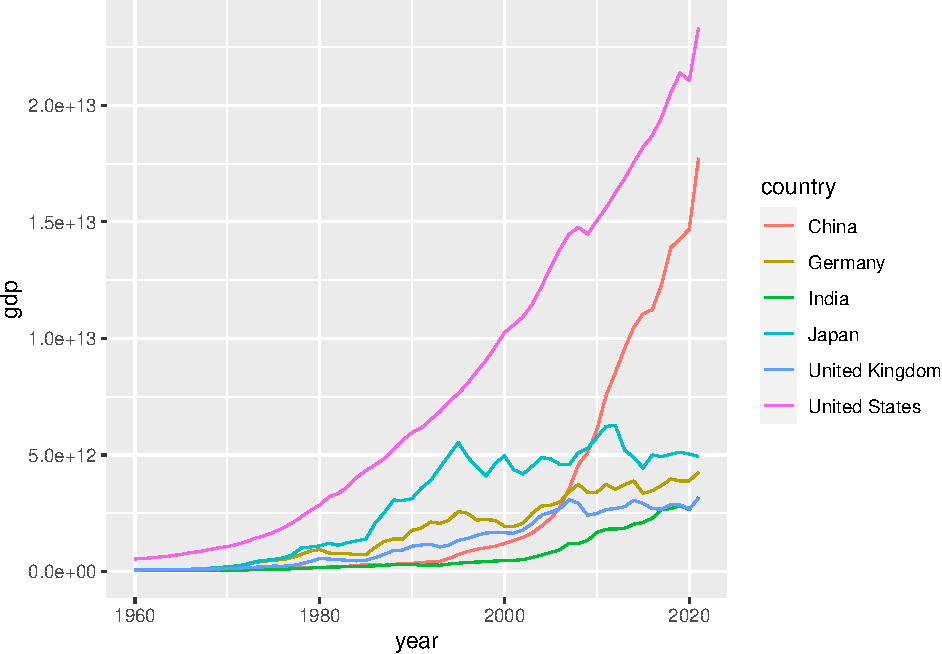
\includegraphics{31-worldbank_files/figure-latex/unnamed-chunk-39-1.pdf}

Warning として、missing values があると出ています。どこかは、分かりませんが、図を書くときですから、\texttt{y} に対応する、\texttt{gdp} の値がないものと思われます。

\hypertarget{ux30b0ux30e9ux30d5-2}{%
\subsubsection{グラフ 2}\label{ux30b0ux30e9ux30d5-2}}

\texttt{drop\_na(gdp)} で、\texttt{gdp} の値が、NA であるものを削除します。また、\texttt{labs} で、図にタイトルをつけます。

\begin{Shaded}
\begin{Highlighting}[]
\NormalTok{df\_gdp4 }\SpecialCharTok{\%\textgreater{}\%} \FunctionTok{drop\_na}\NormalTok{(gdp) }\SpecialCharTok{\%\textgreater{}\%} 
  \FunctionTok{ggplot}\NormalTok{(}\FunctionTok{aes}\NormalTok{(year, gdp, }\AttributeTok{col=}\NormalTok{country)) }\SpecialCharTok{+} \FunctionTok{geom\_line}\NormalTok{() }\SpecialCharTok{+}
  \FunctionTok{labs}\NormalTok{(}\AttributeTok{title =} \StringTok{"WDI {-} NY.GDP.MKTP.CD: gdp"}\NormalTok{)}
\end{Highlighting}
\end{Shaded}

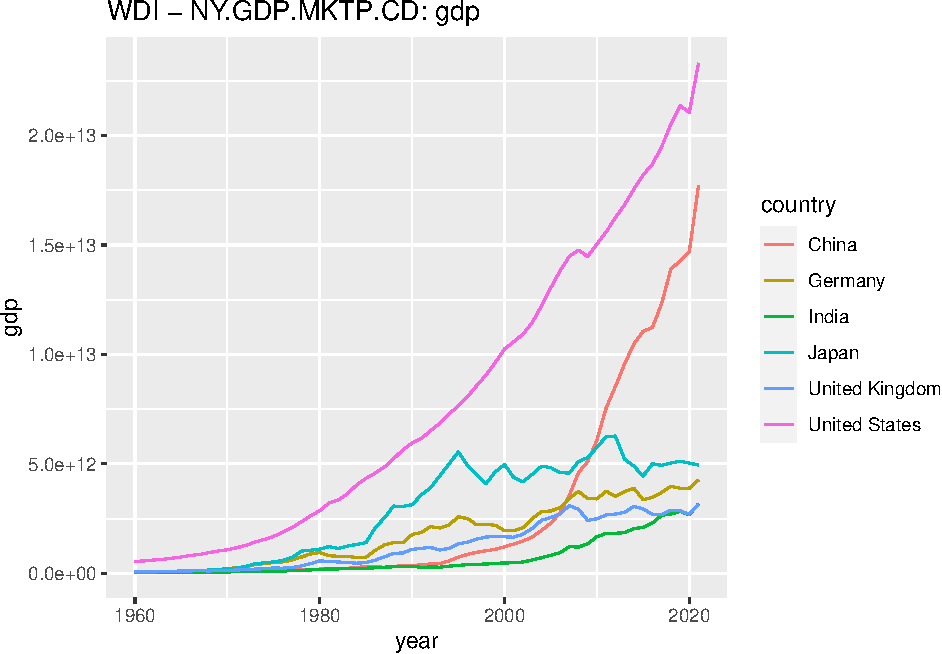
\includegraphics{31-worldbank_files/figure-latex/unnamed-chunk-40-1.pdf}

\hypertarget{ux30c6ux30f3ux30d7ux30ecux30fcux30c8-templates}{%
\subsubsection{テンプレート Templates}\label{ux30c6ux30f3ux30d7ux30ecux30fcux30c8-templates}}

下に、テンプレートをつけます。コピーして、指標コードや、略称、国などを、それぞれ置き換えて、試して見てください。少し、複雑な変形をしていますが、少しずつ説明します。

\hypertarget{ux4e00ux3064ux306eux56fdux306bux3064ux3044ux3066ux306eux4e00ux3064ux306eux6307ux6a19wdiux3068ux305dux306eux7565ux79f0ux304bux3089ux6298ux7ddaux30b0ux30e9ux30d5ux3092ux4f5cux6210}{%
\paragraph{一つの国についての、一つの指標(WDI)と、その略称から、折線グラフを作成}\label{ux4e00ux3064ux306eux56fdux306bux3064ux3044ux3066ux306eux4e00ux3064ux306eux6307ux6a19wdiux3068ux305dux306eux7565ux79f0ux304bux3089ux6298ux7ddaux30b0ux30e9ux30d5ux3092ux4f5cux6210}}

Line Plot with one indicator with abbreviation and one country

\begin{Shaded}
\begin{Highlighting}[]
\NormalTok{chosen\_indicator }\OtherTok{\textless{}{-}} \StringTok{"SL.UEM.TOTL.NE.ZS"}
\NormalTok{short\_name }\OtherTok{\textless{}{-}} \StringTok{"unemployment"}
\NormalTok{chosen\_country }\OtherTok{\textless{}{-}} \StringTok{"United States"}
\FunctionTok{WDI}\NormalTok{(}\AttributeTok{country =} \StringTok{"all"}\NormalTok{, }\AttributeTok{indicator =} \FunctionTok{c}\NormalTok{(}\AttributeTok{short\_name =}\NormalTok{ chosen\_indicator), }\AttributeTok{extra=}\ConstantTok{TRUE}\NormalTok{, }\AttributeTok{cache=}\NormalTok{wdi\_cache) }\SpecialCharTok{\%\textgreater{}\%}
  \FunctionTok{filter}\NormalTok{(country }\SpecialCharTok{==}\NormalTok{ chosen\_country) }\SpecialCharTok{\%\textgreater{}\%} 
  \FunctionTok{ggplot}\NormalTok{(}\FunctionTok{aes}\NormalTok{(year, short\_name)) }\SpecialCharTok{+} \FunctionTok{geom\_line}\NormalTok{() }\SpecialCharTok{+}
  \FunctionTok{labs}\NormalTok{(}\AttributeTok{title =} \FunctionTok{paste}\NormalTok{(}\StringTok{"WDI "}\NormalTok{, chosen\_indicator, }\StringTok{": "}\NormalTok{, short\_name, }\StringTok{" {-} "}\NormalTok{, chosen\_country),}
       \AttributeTok{y =}\NormalTok{ short\_name)}
\end{Highlighting}
\end{Shaded}

\hypertarget{ux4e00ux3064ux306eux56fdux306bux3064ux3044ux3066ux306eux4e00ux3064ux306eux6307ux6a19wdiux304bux3089ux6298ux7ddaux30b0ux30e9ux30d5ux3092ux4f5cux6210}{%
\paragraph{一つの国についての、一つの指標(WDI)から、折線グラフを作成}\label{ux4e00ux3064ux306eux56fdux306bux3064ux3044ux3066ux306eux4e00ux3064ux306eux6307ux6a19wdiux304bux3089ux6298ux7ddaux30b0ux30e9ux30d5ux3092ux4f5cux6210}}

Line Plot with one indicator and one country

\begin{Shaded}
\begin{Highlighting}[]
\NormalTok{chosen\_indicator }\OtherTok{\textless{}{-}} \StringTok{"SL.UEM.TOTL.NE.ZS"}
\NormalTok{chosen\_country }\OtherTok{\textless{}{-}} \StringTok{"United States"}
\FunctionTok{WDI}\NormalTok{(}\AttributeTok{country =} \StringTok{"all"}\NormalTok{, }\AttributeTok{indicator =} \FunctionTok{c}\NormalTok{(}\AttributeTok{chosen\_indicator =}\NormalTok{ chosen\_indicator), }
    \AttributeTok{extra=}\ConstantTok{TRUE}\NormalTok{, }\AttributeTok{cache=}\NormalTok{wdi\_cache) }\SpecialCharTok{\%\textgreater{}\%}
  \FunctionTok{filter}\NormalTok{(country }\SpecialCharTok{==}\NormalTok{ chosen\_country) }\SpecialCharTok{\%\textgreater{}\%} 
  \FunctionTok{ggplot}\NormalTok{(}\FunctionTok{aes}\NormalTok{(year, chosen\_indicator)) }\SpecialCharTok{+} \FunctionTok{geom\_line}\NormalTok{() }\SpecialCharTok{+}
  \FunctionTok{labs}\NormalTok{(}\AttributeTok{title =} \FunctionTok{paste}\NormalTok{(}\StringTok{"WDI "}\NormalTok{, chosen\_indicator, }\StringTok{" {-} "}\NormalTok{, chosen\_country), }
       \AttributeTok{y =}\NormalTok{ chosen\_indicator)}
\end{Highlighting}
\end{Shaded}

\hypertarget{ux3044ux304fux3064ux304bux306eux56fdux306bux3064ux3044ux3066ux306eux4e00ux3064ux306eux6307ux6a19wdiux3068ux305dux306eux7565ux79f0ux304bux3089ux6298ux7ddaux30b0ux30e9ux30d5ux3092ux4f5cux6210}{%
\paragraph{いくつかの国についての、一つの指標(WDI)と、その略称から、折線グラフを作成}\label{ux3044ux304fux3064ux304bux306eux56fdux306bux3064ux3044ux3066ux306eux4e00ux3064ux306eux6307ux6a19wdiux3068ux305dux306eux7565ux79f0ux304bux3089ux6298ux7ddaux30b0ux30e9ux30d5ux3092ux4f5cux6210}}

Line Plot with one indicator with abbreviation and several countries

\begin{Shaded}
\begin{Highlighting}[]
\NormalTok{chosen\_indicator }\OtherTok{\textless{}{-}} \StringTok{"SL.UEM.TOTL.NE.ZS"}
\NormalTok{short\_name }\OtherTok{\textless{}{-}} \StringTok{"unemployment"}
\NormalTok{chosen\_countries }\OtherTok{\textless{}{-}} \FunctionTok{c}\NormalTok{(}\StringTok{"United States"}\NormalTok{,}\StringTok{"United Kingdom"}\NormalTok{, }\StringTok{"Japan"}\NormalTok{)}
\FunctionTok{WDI}\NormalTok{(}\AttributeTok{country =} \StringTok{"all"}\NormalTok{, }\AttributeTok{indicator =} \FunctionTok{c}\NormalTok{(}\AttributeTok{short\_name =}\NormalTok{ chosen\_indicator), }\AttributeTok{extra=}\ConstantTok{TRUE}\NormalTok{, }\AttributeTok{cache=}\NormalTok{wdi\_cache) }\SpecialCharTok{\%\textgreater{}\%} \FunctionTok{drop\_na}\NormalTok{(short\_name) }\SpecialCharTok{\%\textgreater{}\%} 
  \FunctionTok{filter}\NormalTok{(country }\SpecialCharTok{\%in\%}\NormalTok{ chosen\_countries) }\SpecialCharTok{\%\textgreater{}\%} 
  \FunctionTok{ggplot}\NormalTok{(}\FunctionTok{aes}\NormalTok{(year, short\_name, }\AttributeTok{col =}\NormalTok{ country)) }\SpecialCharTok{+} \FunctionTok{geom\_line}\NormalTok{() }\SpecialCharTok{+}
  \FunctionTok{labs}\NormalTok{(}\AttributeTok{title =} \FunctionTok{paste}\NormalTok{(}\StringTok{"WDI "}\NormalTok{, chosen\_indicator, }\StringTok{": "}\NormalTok{, short\_name), }\AttributeTok{y =}\NormalTok{ short\_name)}
\end{Highlighting}
\end{Shaded}

\hypertarget{ux4e00ux3064ux306eux56fdux306bux3064ux3044ux3066ux306eux4e8cux3064ux306eux6307ux6a19wdiux3068ux305dux306eux7565ux79f0ux304bux3089ux6298ux7ddaux30b0ux30e9ux30d5ux3092ux4f5cux6210}{%
\paragraph{一つの国についての、二つの指標(WDI)と、その略称から、折線グラフを作成}\label{ux4e00ux3064ux306eux56fdux306bux3064ux3044ux3066ux306eux4e8cux3064ux306eux6307ux6a19wdiux3068ux305dux306eux7565ux79f0ux304bux3089ux6298ux7ddaux30b0ux30e9ux30d5ux3092ux4f5cux6210}}

Line Plot with two indicators with abbreviation and one country

\begin{Shaded}
\begin{Highlighting}[]
\NormalTok{chosen\_indicator\_1 }\OtherTok{\textless{}{-}} \StringTok{"NY.GDP.DEFL.KD.ZG"}
\NormalTok{short\_name\_1 }\OtherTok{\textless{}{-}} \StringTok{"gdp\_deflator"}
\NormalTok{chosen\_indicator\_2 }\OtherTok{\textless{}{-}} \StringTok{"CPTOTSAXNZGY"}
\NormalTok{short\_name\_2 }\OtherTok{\textless{}{-}} \StringTok{"cpi\_price"}
\NormalTok{chosen\_country }\OtherTok{\textless{}{-}} \StringTok{"United States"}
\FunctionTok{WDI}\NormalTok{(}\AttributeTok{country =} \StringTok{"all"}\NormalTok{, }\AttributeTok{indicator =} \FunctionTok{c}\NormalTok{(}\AttributeTok{short\_name\_1 =}\NormalTok{ chosen\_indicator\_1, }\AttributeTok{short\_name\_2 =}\NormalTok{ chosen\_indicator\_2), }\AttributeTok{extra=}\ConstantTok{TRUE}\NormalTok{, }\AttributeTok{cache=}\NormalTok{wdi\_cache) }\SpecialCharTok{\%\textgreater{}\%} 
  \FunctionTok{filter}\NormalTok{(country }\SpecialCharTok{==}\NormalTok{ chosen\_country) }\SpecialCharTok{\%\textgreater{}\%} 
  \FunctionTok{pivot\_longer}\NormalTok{(}\FunctionTok{c}\NormalTok{(short\_name\_1, short\_name\_2), }\AttributeTok{names\_to =} \StringTok{"class"}\NormalTok{, }\AttributeTok{values\_to =} \StringTok{"value"}\NormalTok{) }\SpecialCharTok{\%\textgreater{}\%} \FunctionTok{drop\_na}\NormalTok{(value) }\SpecialCharTok{\%\textgreater{}\%}
  \FunctionTok{ggplot}\NormalTok{(}\FunctionTok{aes}\NormalTok{(year, value, }\AttributeTok{col =}\NormalTok{ class)) }\SpecialCharTok{+} \FunctionTok{geom\_line}\NormalTok{() }\SpecialCharTok{+}
  \FunctionTok{labs}\NormalTok{(}\AttributeTok{title =} \FunctionTok{paste}\NormalTok{(}\StringTok{"WDI "}\NormalTok{, chosen\_indicator\_1, }\StringTok{": "}\NormalTok{, short\_name\_1, }\StringTok{"}\SpecialCharTok{\textbackslash{}n}\StringTok{"}\NormalTok{, chosen\_indicator\_2, }\StringTok{": "}\NormalTok{, short\_name\_2, }\StringTok{" {-} "}\NormalTok{, chosen\_country)) }\SpecialCharTok{+}
  \FunctionTok{scale\_color\_manual}\NormalTok{(}\AttributeTok{labels =} \FunctionTok{c}\NormalTok{(short\_name\_1, short\_name\_2), }\AttributeTok{values =}\NormalTok{ scales}\SpecialCharTok{::}\FunctionTok{hue\_pal}\NormalTok{()(}\DecValTok{2}\NormalTok{))}
\end{Highlighting}
\end{Shaded}

\begin{Shaded}
\begin{Highlighting}[]
\NormalTok{chosen\_indicator\_1 }\OtherTok{\textless{}{-}} \StringTok{"SL.TLF.CACT.MA.NE.ZS"}
\NormalTok{short\_name\_1 }\OtherTok{\textless{}{-}} \StringTok{"male"}
\NormalTok{chosen\_indicator\_2 }\OtherTok{\textless{}{-}} \StringTok{"SL.TLF.CACT.FE.NE.ZS"}
\NormalTok{short\_name\_2 }\OtherTok{\textless{}{-}} \StringTok{"female"}
\NormalTok{chosen\_country }\OtherTok{\textless{}{-}} \StringTok{"United States"}
\FunctionTok{WDI}\NormalTok{(}\AttributeTok{country =} \StringTok{"all"}\NormalTok{, }\AttributeTok{indicator =} \FunctionTok{c}\NormalTok{(}\AttributeTok{short\_name\_1 =}\NormalTok{ chosen\_indicator\_1, }\AttributeTok{short\_name\_2 =}\NormalTok{ chosen\_indicator\_2), }\AttributeTok{extra=}\ConstantTok{TRUE}\NormalTok{, }\AttributeTok{cache=}\NormalTok{wdi\_cache) }\SpecialCharTok{\%\textgreater{}\%} 
  \FunctionTok{filter}\NormalTok{(country }\SpecialCharTok{==}\NormalTok{ chosen\_country) }\SpecialCharTok{\%\textgreater{}\%} 
  \FunctionTok{pivot\_longer}\NormalTok{(}\FunctionTok{c}\NormalTok{(short\_name\_1, short\_name\_2), }\AttributeTok{names\_to =} \StringTok{"class"}\NormalTok{, }\AttributeTok{values\_to =} \StringTok{"value"}\NormalTok{) }\SpecialCharTok{\%\textgreater{}\%} \FunctionTok{drop\_na}\NormalTok{(value) }\SpecialCharTok{\%\textgreater{}\%}
  \FunctionTok{ggplot}\NormalTok{(}\FunctionTok{aes}\NormalTok{(year, value, }\AttributeTok{col =}\NormalTok{ class)) }\SpecialCharTok{+} \FunctionTok{geom\_line}\NormalTok{() }\SpecialCharTok{+}
  \FunctionTok{labs}\NormalTok{(}\AttributeTok{title =} \FunctionTok{paste}\NormalTok{(}\StringTok{"WDI "}\NormalTok{, chosen\_indicator\_1, }\StringTok{": "}\NormalTok{, short\_name\_1, }\StringTok{"}\SpecialCharTok{\textbackslash{}n}\StringTok{"}\NormalTok{, chosen\_indicator\_2, }\StringTok{": "}\NormalTok{, short\_name\_2, }\StringTok{" {-} "}\NormalTok{, chosen\_country)) }\SpecialCharTok{+}
  \FunctionTok{scale\_color\_manual}\NormalTok{(}\AttributeTok{labels =} \FunctionTok{c}\NormalTok{(short\_name\_1, short\_name\_2), }\AttributeTok{values =}\NormalTok{ scales}\SpecialCharTok{::}\FunctionTok{hue\_pal}\NormalTok{()(}\DecValTok{2}\NormalTok{))}
\end{Highlighting}
\end{Shaded}

\hypertarget{ux3044ux304fux3064ux304bux306eux56fdux306bux3064ux3044ux3066ux306eux4e8cux3064ux306eux6307ux6a19wdiux3068ux305dux306eux7565ux79f0ux304bux3089ux6298ux7ddaux30b0ux30e9ux30d5ux3092ux4f5cux6210}{%
\paragraph{いくつかの国についての、二つの指標(WDI)と、その略称から、折線グラフを作成}\label{ux3044ux304fux3064ux304bux306eux56fdux306bux3064ux3044ux3066ux306eux4e8cux3064ux306eux6307ux6a19wdiux3068ux305dux306eux7565ux79f0ux304bux3089ux6298ux7ddaux30b0ux30e9ux30d5ux3092ux4f5cux6210}}

Line Plot with two indicators with abbreviation and several countries

\begin{Shaded}
\begin{Highlighting}[]
\NormalTok{chosen\_indicator\_1 }\OtherTok{\textless{}{-}} \StringTok{"NY.GDP.DEFL.KD.ZG"}
\NormalTok{short\_name\_1 }\OtherTok{\textless{}{-}} \StringTok{"gdp\_deflator"}
\NormalTok{chosen\_indicator\_2 }\OtherTok{\textless{}{-}} \StringTok{"CPTOTSAXNZGY"}
\NormalTok{short\_name\_2 }\OtherTok{\textless{}{-}} \StringTok{"cpi\_price"}
\NormalTok{chosen\_countries }\OtherTok{\textless{}{-}} \FunctionTok{c}\NormalTok{(}\StringTok{"United States"}\NormalTok{, }\StringTok{"France"}\NormalTok{, }\StringTok{"Japan"}\NormalTok{)}
\FunctionTok{WDI}\NormalTok{(}\AttributeTok{country =} \StringTok{"all"}\NormalTok{, }\AttributeTok{indicator =} \FunctionTok{c}\NormalTok{(}\AttributeTok{short\_name\_1 =}\NormalTok{ chosen\_indicator\_1, }\AttributeTok{short\_name\_2 =}\NormalTok{ chosen\_indicator\_2), }\AttributeTok{extra=}\ConstantTok{TRUE}\NormalTok{, }\AttributeTok{cache=}\NormalTok{wdi\_cache) }\SpecialCharTok{\%\textgreater{}\%} 
  \FunctionTok{filter}\NormalTok{(country }\SpecialCharTok{\%in\%}\NormalTok{ chosen\_countries) }\SpecialCharTok{\%\textgreater{}\%} 
  \FunctionTok{pivot\_longer}\NormalTok{(}\FunctionTok{c}\NormalTok{(short\_name\_1, short\_name\_2), }\AttributeTok{names\_to =} \StringTok{"class"}\NormalTok{, }\AttributeTok{values\_to =} \StringTok{"value"}\NormalTok{) }\SpecialCharTok{\%\textgreater{}\%} \FunctionTok{drop\_na}\NormalTok{(value) }\SpecialCharTok{\%\textgreater{}\%}
  \FunctionTok{ggplot}\NormalTok{(}\FunctionTok{aes}\NormalTok{(year, value, }\AttributeTok{linetype =}\NormalTok{ class, }\AttributeTok{col =}\NormalTok{ country)) }\SpecialCharTok{+} \FunctionTok{geom\_line}\NormalTok{() }\SpecialCharTok{+}
  \FunctionTok{labs}\NormalTok{(}\AttributeTok{title =} \FunctionTok{paste}\NormalTok{(}\StringTok{"WDI "}\NormalTok{, chosen\_indicator\_1, }\StringTok{": "}\NormalTok{, short\_name\_1, }\StringTok{"}\SpecialCharTok{\textbackslash{}n}\StringTok{"}\NormalTok{, chosen\_indicator\_2, }\StringTok{": "}\NormalTok{, short\_name\_2)) }\SpecialCharTok{+}
  \FunctionTok{scale\_linetype\_manual}\NormalTok{(}\AttributeTok{labels =} \FunctionTok{c}\NormalTok{(short\_name\_1, short\_name\_2), }\AttributeTok{values =} \FunctionTok{c}\NormalTok{(}\StringTok{"solid"}\NormalTok{, }\StringTok{"dashed"}\NormalTok{))}
\end{Highlighting}
\end{Shaded}

\begin{Shaded}
\begin{Highlighting}[]
\NormalTok{chosen\_indicator\_1 }\OtherTok{\textless{}{-}} \StringTok{"SL.TLF.CACT.MA.NE.ZS"}
\NormalTok{short\_name\_1 }\OtherTok{\textless{}{-}} \StringTok{"male"}
\NormalTok{chosen\_indicator\_2 }\OtherTok{\textless{}{-}} \StringTok{"SL.TLF.CACT.FE.NE.ZS"}
\NormalTok{short\_name\_2 }\OtherTok{\textless{}{-}} \StringTok{"female"}
\NormalTok{chosen\_countries }\OtherTok{\textless{}{-}} \FunctionTok{c}\NormalTok{(}\StringTok{"United States"}\NormalTok{, }\StringTok{"France"}\NormalTok{, }\StringTok{"Japan"}\NormalTok{)}
\FunctionTok{WDI}\NormalTok{(}\AttributeTok{country =} \StringTok{"all"}\NormalTok{, }\AttributeTok{indicator =} \FunctionTok{c}\NormalTok{(}\AttributeTok{short\_name\_1 =}\NormalTok{ chosen\_indicator\_1, }\AttributeTok{short\_name\_2 =}\NormalTok{ chosen\_indicator\_2), }\AttributeTok{extra=}\ConstantTok{TRUE}\NormalTok{, }\AttributeTok{cache=}\NormalTok{wdi\_cache) }\SpecialCharTok{\%\textgreater{}\%} 
  \FunctionTok{filter}\NormalTok{(country }\SpecialCharTok{\%in\%}\NormalTok{ chosen\_countries) }\SpecialCharTok{\%\textgreater{}\%} 
  \FunctionTok{pivot\_longer}\NormalTok{(}\FunctionTok{c}\NormalTok{(short\_name\_1, short\_name\_2), }\AttributeTok{names\_to =} \StringTok{"class"}\NormalTok{, }\AttributeTok{values\_to =} \StringTok{"value"}\NormalTok{) }\SpecialCharTok{\%\textgreater{}\%} \FunctionTok{drop\_na}\NormalTok{(value) }\SpecialCharTok{\%\textgreater{}\%}
  \FunctionTok{ggplot}\NormalTok{(}\FunctionTok{aes}\NormalTok{(year, value, }\AttributeTok{linetype =}\NormalTok{ class, }\AttributeTok{col =}\NormalTok{ country)) }\SpecialCharTok{+} \FunctionTok{geom\_line}\NormalTok{() }\SpecialCharTok{+}
  \FunctionTok{labs}\NormalTok{(}\AttributeTok{title =} \FunctionTok{paste}\NormalTok{(}\StringTok{"WDI "}\NormalTok{, chosen\_indicator\_1, }\StringTok{": "}\NormalTok{, short\_name\_1, }\StringTok{"}\SpecialCharTok{\textbackslash{}n}\StringTok{"}\NormalTok{, chosen\_indicator\_2, }\StringTok{": "}\NormalTok{, short\_name\_2)) }\SpecialCharTok{+}
  \FunctionTok{scale\_linetype\_manual}\NormalTok{(}\AttributeTok{labels =} \FunctionTok{c}\NormalTok{(short\_name\_1, short\_name\_2), }\AttributeTok{values =} \FunctionTok{c}\NormalTok{(}\StringTok{"solid"}\NormalTok{, }\StringTok{"dashed"}\NormalTok{))}
\end{Highlighting}
\end{Shaded}

\hypertarget{ux8ab2ux984c-assignment}{%
\subsection{課題 Assignment}\label{ux8ab2ux984c-assignment}}

上のテンプレートをコピーして、下に貼り付け、指標 \texttt{indicator} と、略称 \texttt{short\_name} と、いくつかの国名 \texttt{chosen\_countries} を、入れ替えて、試してみてください。

\hypertarget{part-part-iv-eda}{%
\part{PART IV EDA}\label{part-part-iv-eda}}

\hypertarget{intro2eda}{%
\section{What is EDA?}\label{intro2eda}}

\hypertarget{part-part-v-examples}{%
\part{PART V EXAMPLES}\label{part-part-v-examples}}

\hypertarget{example1}{%
\section{Example 1}\label{example1}}

\hypertarget{appendix-appendix}{%
\appendix}


\hypertarget{japanese}{%
\section{日本語の扱いについて}\label{japanese}}

\hypertarget{ux65e5ux672cux8a9eux4e2dux56fdux8a9eux97d3ux56fdux8a9e}{%
\subsection{日本語・中国語・韓国語}\label{ux65e5ux672cux8a9eux4e2dux56fdux8a9eux97d3ux56fdux8a9e}}

文字化けが、起こることが多く、対応が、一定せず、難しかったのですが、どうやら、現在は、どの場合も、次の設定で、解決しているようです。下の例を確認してください。

\begin{Shaded}
\begin{Highlighting}[]
\CommentTok{\# showtext を、インストールしていない場合は、一回だけ、右上の三角をクリックして実行}
\FunctionTok{install.packages}\NormalTok{(}\StringTok{\textquotesingle{}showtext\textquotesingle{}}\NormalTok{)}
\end{Highlighting}
\end{Shaded}

\hypertarget{ux30d1ux30c3ux30b1ux30fcux30b8ux3092ux30edux30fcux30c9}{%
\subsubsection{パッケージをロード}\label{ux30d1ux30c3ux30b1ux30fcux30b8ux3092ux30edux30fcux30c9}}

\texttt{library} によって、Package をロード(いつでも使えるように)します。

\begin{Shaded}
\begin{Highlighting}[]
\FunctionTok{library}\NormalTok{(tidyverse)}
\FunctionTok{library}\NormalTok{(showtext) }
\FunctionTok{font\_add\_google}\NormalTok{(}\StringTok{\textquotesingle{}Noto Sans\textquotesingle{}}\NormalTok{)}
\FunctionTok{showtext\_auto}\NormalTok{()}
\end{Highlighting}
\end{Shaded}

\hypertarget{base-r-ux3067ux30bfux30a4ux30c8ux30ebux306bux65e5ux672cux8a9e}{%
\subsection{Base R でタイトルに日本語}\label{base-r-ux3067ux30bfux30a4ux30c8ux30ebux306bux65e5ux672cux8a9e}}

\begin{Shaded}
\begin{Highlighting}[]
\FunctionTok{plot}\NormalTok{(cars, }\AttributeTok{main=}\StringTok{"散布図"}\NormalTok{)}
\end{Highlighting}
\end{Shaded}

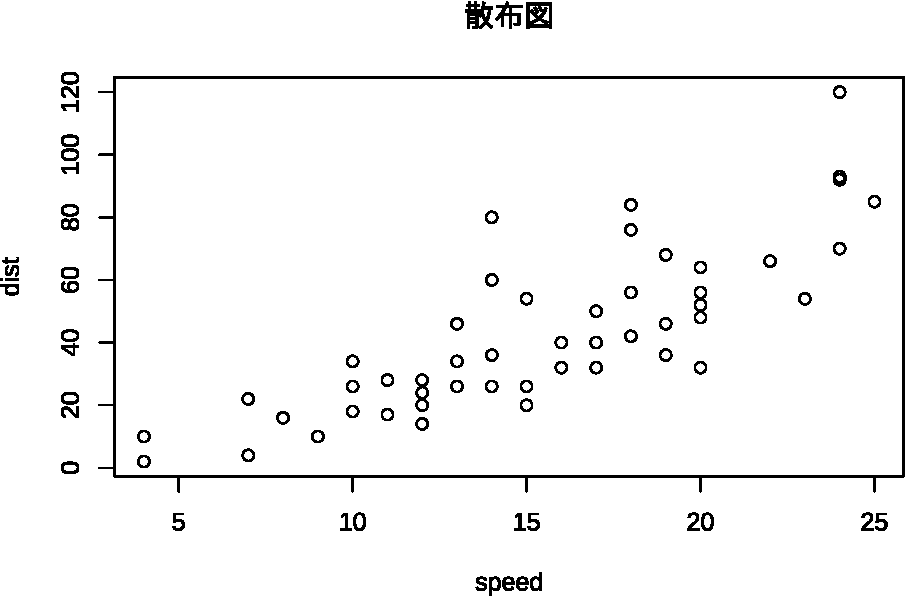
\includegraphics{81-japanese_files/figure-latex/unnamed-chunk-3-1.pdf}

\hypertarget{ux5217ux540dux3084ux30c7ux30fcux30bfux306bux65e5ux672cux8a9e}{%
\subsection{列名や、データに日本語}\label{ux5217ux540dux3084ux30c7ux30fcux30bfux306bux65e5ux672cux8a9e}}

\begin{Shaded}
\begin{Highlighting}[]
\NormalTok{df\_iris }\OtherTok{\textless{}{-}}\NormalTok{ iris}
\FunctionTok{colnames}\NormalTok{(df\_iris) }\OtherTok{\textless{}{-}} \FunctionTok{c}\NormalTok{(}\StringTok{"萼長"}\NormalTok{,}\StringTok{"萼幅"}\NormalTok{,}\StringTok{"葉長"}\NormalTok{,}\StringTok{"葉幅"}\NormalTok{,}\StringTok{"Species"}\NormalTok{ )}
\NormalTok{tab }\OtherTok{\textless{}{-}} \FunctionTok{data.frame}\NormalTok{(}\AttributeTok{Species =} \FunctionTok{c}\NormalTok{(}\StringTok{"setosa"}\NormalTok{, }\StringTok{"versicolor"}\NormalTok{, }\StringTok{"virginica"}\NormalTok{), }
                  \StringTok{"種別"} \OtherTok{=} \FunctionTok{c}\NormalTok{(}\StringTok{"ヒオウギアヤメ"}\NormalTok{, }\StringTok{"ブルーフラッグ"}\NormalTok{, }\StringTok{"バージニカ"}\NormalTok{))}
\NormalTok{df\_iris }\OtherTok{\textless{}{-}}\NormalTok{ df\_iris }\SpecialCharTok{\%\textgreater{}\%} \FunctionTok{left\_join}\NormalTok{(tab, }\AttributeTok{by=}\FunctionTok{c}\NormalTok{(}\StringTok{"Species"} \OtherTok{=} \StringTok{"Species"}\NormalTok{)) }\SpecialCharTok{\%\textgreater{}\%} \FunctionTok{select}\NormalTok{(}\SpecialCharTok{{-}}\DecValTok{5}\NormalTok{)}
\NormalTok{df\_iris }\SpecialCharTok{\%\textgreater{}\%} \FunctionTok{slice}\NormalTok{(}\DecValTok{1}\SpecialCharTok{:}\DecValTok{2}\NormalTok{)}
\CommentTok{\#\textgreater{}   萼長 萼幅 葉長 葉幅           種別}
\CommentTok{\#\textgreater{} 1  5.1  3.5  1.4  0.2 ヒオウギアヤメ}
\CommentTok{\#\textgreater{} 2  4.9  3.0  1.4  0.2 ヒオウギアヤメ}
\end{Highlighting}
\end{Shaded}

\hypertarget{kable-ux3067ux8868ux793a}{%
\subsection{\texorpdfstring{\texttt{kable} で表示}{kable で表示}}\label{kable-ux3067ux8868ux793a}}

\begin{Shaded}
\begin{Highlighting}[]
\NormalTok{knitr}\SpecialCharTok{::}\FunctionTok{kable}\NormalTok{(df\_iris[}\DecValTok{1}\SpecialCharTok{:}\DecValTok{6}\NormalTok{, ])}
\end{Highlighting}
\end{Shaded}

\begin{tabular}{r|r|r|r|l}
\hline
萼長 & 萼幅 & 葉長 & 葉幅 & 種別\\
\hline
5.1 & 3.5 & 1.4 & 0.2 & ヒオウギアヤメ\\
\hline
4.9 & 3.0 & 1.4 & 0.2 & ヒオウギアヤメ\\
\hline
4.7 & 3.2 & 1.3 & 0.2 & ヒオウギアヤメ\\
\hline
4.6 & 3.1 & 1.5 & 0.2 & ヒオウギアヤメ\\
\hline
5.0 & 3.6 & 1.4 & 0.2 & ヒオウギアヤメ\\
\hline
5.4 & 3.9 & 1.7 & 0.4 & ヒオウギアヤメ\\
\hline
\end{tabular}

\hypertarget{ggplot-ux3067ux30b0ux30e9ux30d5ux3092ux4f5cux6210}{%
\subsection{\texorpdfstring{\texttt{ggplot} でグラフを作成}{ggplot でグラフを作成}}\label{ggplot-ux3067ux30b0ux30e9ux30d5ux3092ux4f5cux6210}}

\begin{Shaded}
\begin{Highlighting}[]
\FunctionTok{ggplot}\NormalTok{(df\_iris, }\FunctionTok{aes}\NormalTok{(}\AttributeTok{x =} \StringTok{\textasciigrave{}}\AttributeTok{葉長}\StringTok{\textasciigrave{}}\NormalTok{, }\AttributeTok{y =} \StringTok{\textasciigrave{}}\AttributeTok{葉幅}\StringTok{\textasciigrave{}}\NormalTok{, }\AttributeTok{col =} \StringTok{\textasciigrave{}}\AttributeTok{種別}\StringTok{\textasciigrave{}}\NormalTok{)) }\SpecialCharTok{+}
  \FunctionTok{geom\_point}\NormalTok{() }\SpecialCharTok{+} \FunctionTok{labs}\NormalTok{(}\AttributeTok{title =} \StringTok{"散布図"}\NormalTok{, }\AttributeTok{x =} \StringTok{"葉長"}\NormalTok{, }\AttributeTok{y =} \StringTok{"葉幅"}\NormalTok{)}
\end{Highlighting}
\end{Shaded}

\includegraphics{81-japanese_files/figure-latex/unnamed-chunk-5-1.pdf}

\hypertarget{ux5099ux8003-1}{%
\subsection{備考:}\label{ux5099ux8003-1}}

実は、一番難しいのが、PDF の作成だと思いますが、一応、上のものも、PDF を作成することが可能です。
下のリンクのファイルを、いろいろな、形式で、出力してみてください。R Notebook と、PDF に出力したもののリンクを付けておきます。

\begin{itemize}
\tightlist
\item
  \href{https://ds-sl.github.io/intro2r/Rmarkdown-J.nb.html}{R Notebook}

  \begin{itemize}
  \tightlist
  \item
    右上の Code ボタンから、Rmd ファイルも取得できます。
  \end{itemize}
\item
  \href{https://ds-sl.github.io/intro2r/Rmarkdown-J.pdf}{PDF}
\end{itemize}

\hypertarget{ux53c2ux8003ux65e5ux672cux8a9eux306eux8868ux793aux306bux3064ux3044ux3066}{%
\subsection{参考:日本語の表示について}\label{ux53c2ux8003ux65e5ux672cux8a9eux306eux8868ux793aux306bux3064ux3044ux3066}}

\begin{quote}
日本語が適切に表示されない!?
\end{quote}

簡単ではなく、未解決の部分が何かなどを含め、わたしも十分理解できているか不明であるが、理解できていると思われる範囲で、備忘録のように記す。

R を使うという場合に限っても、R Studio IDE を使う場合、RStudio Cloud を使う場合、Google colab を使う場合、他のプラットフォームで使う場合で違ってくると思われる。一応、上にあげた、三種類のプラットフォームで確かめられるものについて書いていく。上に書いた以外に、R Studio IDE を、Windows 上で使う場合と、Mac 上で使う場合(Mac のシステムは Unix 系であるが、さまざまな Linux )でも、状況が異なる。そこで、場合分けをして書いていくほうが安全であるが、それは、極力避け、どれにでも適用可能な方法を模索しながら書いていこうと思っている。個人的に、日常的に分断を避ける努力をすることが大切だとおもっていることも背景にある。さらに、ソフトウェア開発者は、むろん、そのような差異を理解して、どの環境でも、可能なように設計することを心がけていると思われるし、そのようなものが、R Project の正規のパッケージとして採用されていくべきだとも考えているので、多少、理想も入っているが、これを基本として書いていこうと思う。十分なチェックができていないものもあるので、不具合などは、ぜひ、お知らせ願いたい。この文章も少しずつ、改善していければと思う。

通常、日本語、中国語、韓国語などが適切に表示できない場合は、文字のエンコーディング(Encoding: どのような情報として記録されているか)と、フォントの問題、さらに、システムがこれらをどう処理しているかの問題があると思われる。しかし、R の利用者として考えると、文字化けが起きたり、適切に文字が表示されないのは、以下の三つに分けられるように思われる。

\begin{enumerate}
\def\labelenumi{\arabic{enumi}.}
\tightlist
\item
  データファイルなどを読み込んだときに適切に表示されない
\item
  図の中のタイトルなどが、適切に表示されない
\item
  R Markdown の出力において、適切に表示されない
\end{enumerate}

\hypertarget{ux30c7ux30fcux30bfux30d5ux30a1ux30a4ux30ebux306eux8aadux307fux8fbcux307f}{%
\subsubsection{データファイルの読み込み}\label{ux30c7ux30fcux30bfux30d5ux30a1ux30a4ux30ebux306eux8aadux307fux8fbcux307f}}

\begin{itemize}
\tightlist
\item
  tidyverse に含まれる readr には、guess\_encoding が含まれており、一般的には、たとえば、

  \begin{itemize}
  \tightlist
  \item
    read\_csv(``./data/file\_name.csv'') とすると、一番可能性の高いエンコーディングで読み込まれる。
  \end{itemize}
\item
  使い方:guess\_encoding(file, n\_max = 10000, threshold = 0.2) とあり、10000行で推測されたエンコーディング、または、確率を計算することを Default にしている。Help によると、すべての行をチェックする場合は、n\_max = -1 とすることが書かれている。
\item
  これで問題がない場合が多い。他の、readr 関数も同様である。
\item
  なお、read\_csv などにも、guess\_max = min(1000, n\_max) も含まれるが、これは、column type を決めるためのものである。
\item
  read.csv() など、base R では、fileEncoding = ````, encoding =''unknown'' がオプションに含まれていたので、指定して読み込むことが通常であった。
\end{itemize}

\hypertarget{ux56f3ux306eux4e2dux306eux30c6ux30adux30b9ux30c8}{%
\subsubsection{図の中のテキスト}\label{ux56f3ux306eux4e2dux306eux30c6ux30adux30b9ux30c8}}

\begin{itemize}
\tightlist
\item
  基本的には、図の表示の前にlibrary(showtext); font\_add\_google(`Noto Sans'); showtext\_auto() となっていれば、これ以降の図は、Google Fonts `Noto Sans' が使われ、表示されるはずである。
\item
  二種類以上のフォントを使い分けたいときは、名前をつけて、それを family = name で指定する。

  \begin{itemize}
  \tightlist
  \item
    showtext: Using Fonts More Easily in R Graphs 参照。
  \end{itemize}
\end{itemize}

\hypertarget{r-markdown-ux306eux51faux529b}{%
\subsubsection{R Markdown の出力}\label{r-markdown-ux306eux51faux529b}}

\begin{itemize}
\tightlist
\item
  PDF 作成における問題が最後まで残っていたが、最近は、showtext Package で解決しているようである。設定については、図の中のテキストの場合と同じ。
\end{itemize}

\hypertarget{ux53c2ux8003ux3068ux3057ux305fux3082ux306e}{%
\subsubsection{参考としたもの}\label{ux53c2ux8003ux3068ux3057ux305fux3082ux306e}}

\hypertarget{showtext-using-fonts-more-easily-in-r-graphs}{%
\paragraph{showtext: Using Fonts More Easily in R Graphs}\label{showtext-using-fonts-more-easily-in-r-graphs}}

\begin{itemize}
\tightlist
\item
  \url{https://CRAN.R-project.org/package=showtext}

  \begin{itemize}
  \tightlist
  \item
    \url{https://cran.r-project.org/web/packages/showtext/readme/README.html}
  \item
    showtext: Using Fonts More Easily in R Graphs:

    \begin{itemize}
    \tightlist
    \item
      \url{https://cran.r-project.org/web/packages/showtext/vignettes/introduction.html}
    \item
      \url{https://fonts.google.com}
    \end{itemize}
  \end{itemize}
\end{itemize}

\hypertarget{sysfonts-loading-fonts-into-r}{%
\paragraph{sysfonts: Loading Fonts into R}\label{sysfonts-loading-fonts-into-r}}

\begin{itemize}
\tightlist
\item
  \url{https://CRAN.R-project.org/package=sysfonts}

  \begin{itemize}
  \tightlist
  \item
    \url{https://cran.r-project.org/web/packages/sysfonts/sysfonts.pdf}
  \end{itemize}
\end{itemize}

\hypertarget{foods4all-examples-of-graphs}{%
\paragraph{foods4all: Examples of Graphs}\label{foods4all-examples-of-graphs}}

\begin{itemize}
\tightlist
\item
  \url{https://foods4all.github.io/examples/examples_of_graphs.html}

  \begin{itemize}
  \tightlist
  \item
    77.2 Japanese Environments 日本語環境(昔の記事:Last Updated: 2020-04-22)
  \end{itemize}
\end{itemize}

\hypertarget{bookdown}{%
\section{Bookdown}\label{bookdown}}

\hypertarget{about}{%
\subsection{About}\label{about}}

This is a \emph{sample} book written in \textbf{Markdown}. You can use anything that Pandoc's Markdown supports; for example, a math equation \(a^2 + b^2 = c^2\).

\hypertarget{usage}{%
\subsubsection{Usage}\label{usage}}

Each \textbf{bookdown} chapter is an .Rmd file, and each .Rmd file can contain one (and only one) chapter. A chapter \emph{must} start with a first-level heading: \texttt{\#\ A\ good\ chapter}, and can contain one (and only one) first-level heading.

Use second-level and higher headings within chapters like: \texttt{\#\#\ A\ short\ section} or \texttt{\#\#\#\ An\ even\ shorter\ section}.

The \texttt{index.Rmd} file is required, and is also your first book chapter. It will be the homepage when you render the book.

\hypertarget{render-book}{%
\subsubsection{Render book}\label{render-book}}

You can render the HTML version of this example book without changing anything:

\begin{enumerate}
\def\labelenumi{\arabic{enumi}.}
\item
  Find the \textbf{Build} pane in the RStudio IDE, and
\item
  Click on \textbf{Build Book}, then select your output format, or select ``All formats'' if you'd like to use multiple formats from the same book source files.
\end{enumerate}

Or build the book from the R console:

\begin{Shaded}
\begin{Highlighting}[]
\NormalTok{bookdown}\SpecialCharTok{::}\FunctionTok{render\_book}\NormalTok{()}
\end{Highlighting}
\end{Shaded}

To render this example to PDF as a \texttt{bookdown::pdf\_book}, you'll need to install XeLaTeX. You are recommended to install TinyTeX (which includes XeLaTeX): \url{https://yihui.org/tinytex/}.

\hypertarget{preview-book}{%
\subsubsection{Preview book}\label{preview-book}}

As you work, you may start a local server to live preview this HTML book. This preview will update as you edit the book when you save individual .Rmd files. You can start the server in a work session by using the RStudio add-in ``Preview book'', or from the R console:

\begin{Shaded}
\begin{Highlighting}[]
\NormalTok{bookdown}\SpecialCharTok{::}\FunctionTok{serve\_book}\NormalTok{()}
\end{Highlighting}
\end{Shaded}

\hypertarget{hello-bookdown}{%
\subsection{Hello bookdown}\label{hello-bookdown}}

All chapters start with a first-level heading followed by your chapter title, like the line above. There should be only one first-level heading (\texttt{\#}) per .Rmd file.

\hypertarget{a-section}{%
\subsubsection{A section}\label{a-section}}

All chapter sections start with a second-level (\texttt{\#\#}) or higher heading followed by your section title, like the sections above and below here. You can have as many as you want within a chapter.

\hypertarget{an-unnumbered-section}{%
\paragraph*{An unnumbered section}\label{an-unnumbered-section}}
\addcontentsline{toc}{paragraph}{An unnumbered section}

Chapters and sections are numbered by default. To un-number a heading, add a \texttt{\{.unnumbered\}} or the shorter \texttt{\{-\}} at the end of the heading, like in this section.

\hypertarget{cross}{%
\subsection{Cross-references}\label{cross}}

Cross-references make it easier for your readers to find and link to elements in your book.

\hypertarget{chapters-and-sub-chapters}{%
\subsubsection{Chapters and sub-chapters}\label{chapters-and-sub-chapters}}

There are two steps to cross-reference any heading:

\begin{enumerate}
\def\labelenumi{\arabic{enumi}.}
\tightlist
\item
  Label the heading: \texttt{\#\ Hello\ world\ \{\#nice-label\}}.

  \begin{itemize}
  \tightlist
  \item
    Leave the label off if you like the automated heading generated based on your heading title: for example, \texttt{\#\ Hello\ world} = \texttt{\#\ Hello\ world\ \{\#hello-world\}}.
  \item
    To label an un-numbered heading, use: \texttt{\#\ Hello\ world\ \{-\#nice-label\}} or \texttt{\{\#\ Hello\ world\ .unnumbered\}}.
  \end{itemize}
\item
  Next, reference the labeled heading anywhere in the text using \texttt{\textbackslash{}@ref(nice-label)}; for example, please see Chapter \ref{cross}.

  \begin{itemize}
  \tightlist
  \item
    If you prefer text as the link instead of a numbered reference use: \protect\hyperlink{cross}{any text you want can go here}.
  \end{itemize}
\end{enumerate}

\hypertarget{captioned-figures-and-tables}{%
\subsubsection{Captioned figures and tables}\label{captioned-figures-and-tables}}

Figures and tables \emph{with captions} can also be cross-referenced from elsewhere in your book using \texttt{\textbackslash{}@ref(fig:chunk-label)} and \texttt{\textbackslash{}@ref(tab:chunk-label)}, respectively.

See Figure \ref{fig:nice-fig}.

\begin{Shaded}
\begin{Highlighting}[]
\FunctionTok{par}\NormalTok{(}\AttributeTok{mar =} \FunctionTok{c}\NormalTok{(}\DecValTok{4}\NormalTok{, }\DecValTok{4}\NormalTok{, .}\DecValTok{1}\NormalTok{, .}\DecValTok{1}\NormalTok{))}
\FunctionTok{plot}\NormalTok{(pressure, }\AttributeTok{type =} \StringTok{\textquotesingle{}b\textquotesingle{}}\NormalTok{, }\AttributeTok{pch =} \DecValTok{19}\NormalTok{)}
\end{Highlighting}
\end{Shaded}

\begin{figure}

{\centering 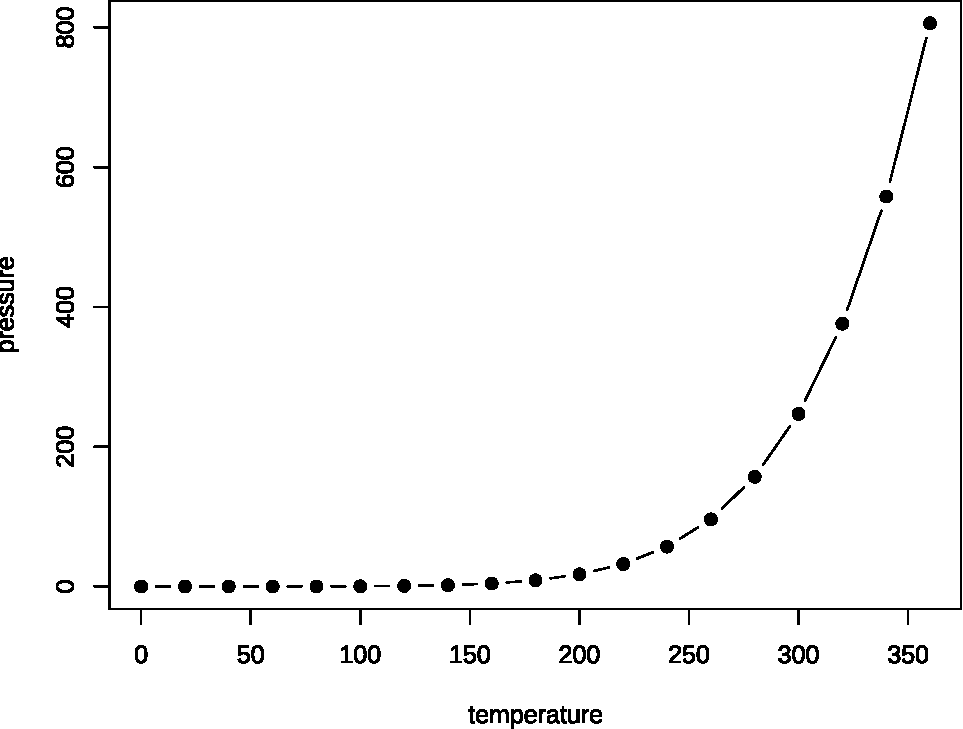
\includegraphics[width=0.8\linewidth]{90-bookdown_files/figure-latex/nice-fig-1} 

}

\caption{Here is a nice figure!}\label{fig:nice-fig}
\end{figure}

Don't miss Table \ref{tab:nice-tab}.

\begin{Shaded}
\begin{Highlighting}[]
\NormalTok{knitr}\SpecialCharTok{::}\FunctionTok{kable}\NormalTok{(}
  \FunctionTok{head}\NormalTok{(pressure, }\DecValTok{10}\NormalTok{), }\AttributeTok{caption =} \StringTok{\textquotesingle{}Here is a nice table!\textquotesingle{}}\NormalTok{,}
  \AttributeTok{booktabs =} \ConstantTok{TRUE}
\NormalTok{)}
\end{Highlighting}
\end{Shaded}

\begin{table}

\caption{\label{tab:nice-tab}Here is a nice table!}
\centering
\begin{tabular}[t]{rr}
\toprule
temperature & pressure\\
\midrule
0 & 0.0002\\
20 & 0.0012\\
40 & 0.0060\\
60 & 0.0300\\
80 & 0.0900\\
\addlinespace
100 & 0.2700\\
120 & 0.7500\\
140 & 1.8500\\
160 & 4.2000\\
180 & 8.8000\\
\bottomrule
\end{tabular}
\end{table}

\hypertarget{parts}{%
\subsection{Parts}\label{parts}}

You can add parts to organize one or more book chapters together. Parts can be inserted at the top of an .Rmd file, before the first-level chapter heading in that same file.

Add a numbered part: \texttt{\#\ (PART)\ Act\ one\ \{-\}} (followed by \texttt{\#\ A\ chapter})

Add an unnumbered part: \texttt{\#\ (PART\textbackslash{}*)\ Act\ one\ \{-\}} (followed by \texttt{\#\ A\ chapter})

Add an appendix as a special kind of un-numbered part: \texttt{\#\ (APPENDIX)\ Other\ stuff\ \{-\}} (followed by \texttt{\#\ A\ chapter}). Chapters in an appendix are prepended with letters instead of numbers.

\hypertarget{footnotes-and-citations}{%
\subsection{Footnotes and citations}\label{footnotes-and-citations}}

\hypertarget{footnotes}{%
\subsubsection{Footnotes}\label{footnotes}}

Footnotes are put inside the square brackets after a caret \texttt{\^{}{[}{]}}. Like this one \footnote{This is a footnote.}.

\hypertarget{citations}{%
\subsubsection{Citations}\label{citations}}

Reference items in your bibliography file(s) using \texttt{@key}.

For example, we are using the \textbf{bookdown} package \citep{R-bookdown} (check out the last code chunk in index.Rmd to see how this citation key was added) in this sample book, which was built on top of R Markdown and \textbf{knitr} \citep{xie2015} (this citation was added manually in an external file book.bib).
Note that the \texttt{.bib} files need to be listed in the index.Rmd with the YAML \texttt{bibliography} key.

The \texttt{bs4\_book} theme makes footnotes appear inline when you click on them. In this example book, we added \texttt{csl:\ chicago-fullnote-bibliography.csl} to the \texttt{index.Rmd} YAML, and include the \texttt{.csl} file. To download a new style, we recommend: \url{https://www.zotero.org/styles/}

The RStudio Visual Markdown Editor can also make it easier to insert citations: \url{https://rstudio.github.io/visual-markdown-editing/\#/citations}

\hypertarget{blocks}{%
\subsection{Blocks}\label{blocks}}

\hypertarget{equations}{%
\subsubsection{Equations}\label{equations}}

Here is an equation.

\begin{equation} 
  f\left(k\right) = \binom{n}{k} p^k\left(1-p\right)^{n-k}
  \label{eq:binom}
\end{equation}

You may refer to using \texttt{\textbackslash{}@ref(eq:binom)}, like see Equation \eqref{eq:binom}.

\hypertarget{theorems-and-proofs}{%
\subsubsection{Theorems and proofs}\label{theorems-and-proofs}}

Labeled theorems can be referenced in text using \texttt{\textbackslash{}@ref(thm:tri)}, for example, check out this smart theorem \ref{thm:tri}.

\begin{theorem}
\protect\hypertarget{thm:tri}{}\label{thm:tri}For a right triangle, if \(c\) denotes the \emph{length} of the hypotenuse
and \(a\) and \(b\) denote the lengths of the \textbf{other} two sides, we have
\[a^2 + b^2 = c^2\]
\end{theorem}

Read more here \url{https://bookdown.org/yihui/bookdown/markdown-extensions-by-bookdown.html}.

\hypertarget{callout-blocks}{%
\subsubsection{Callout blocks}\label{callout-blocks}}

The \texttt{bs4\_book} theme also includes special callout blocks, like this \texttt{.rmdnote}.

You can use \textbf{markdown} inside a block.

\begin{Shaded}
\begin{Highlighting}[]
\FunctionTok{head}\NormalTok{(beaver1, }\AttributeTok{n =} \DecValTok{5}\NormalTok{)}
\CommentTok{\#\textgreater{}   day time  temp activ}
\CommentTok{\#\textgreater{} 1 346  840 36.33     0}
\CommentTok{\#\textgreater{} 2 346  850 36.34     0}
\CommentTok{\#\textgreater{} 3 346  900 36.35     0}
\CommentTok{\#\textgreater{} 4 346  910 36.42     0}
\CommentTok{\#\textgreater{} 5 346  920 36.55     0}
\end{Highlighting}
\end{Shaded}

It is up to the user to define the appearance of these blocks for LaTeX output.

You may also use: \texttt{.rmdcaution}, \texttt{.rmdimportant}, \texttt{.rmdtip}, or \texttt{.rmdwarning} as the block name.

The R Markdown Cookbook provides more help on how to use custom blocks to design your own callouts: \url{https://bookdown.org/yihui/rmarkdown-cookbook/custom-blocks.html}

\hypertarget{sharing-your-book}{%
\subsection{Sharing your book}\label{sharing-your-book}}

\hypertarget{publishing}{%
\subsubsection{Publishing}\label{publishing}}

HTML books can be published online, see: \url{https://bookdown.org/yihui/bookdown/publishing.html}

\hypertarget{pages}{%
\subsubsection{404 pages}\label{pages}}

By default, users will be directed to a 404 page if they try to access a webpage that cannot be found. If you'd like to customize your 404 page instead of using the default, you may add either a \texttt{\_404.Rmd} or \texttt{\_404.md} file to your project root and use code and/or Markdown syntax.

\hypertarget{metadata-for-sharing}{%
\subsubsection{Metadata for sharing}\label{metadata-for-sharing}}

Bookdown HTML books will provide HTML metadata for social sharing on platforms like Twitter, Facebook, and LinkedIn, using information you provide in the \texttt{index.Rmd} YAML. To setup, set the \texttt{url} for your book and the path to your \texttt{cover-image} file. Your book's \texttt{title} and \texttt{description} are also used.

This \texttt{bs4\_book} provides enhanced metadata for social sharing, so that each chapter shared will have a unique description, auto-generated based on the content.

Specify your book's source repository on GitHub as the \texttt{repo} in the \texttt{\_output.yml} file, which allows users to view each chapter's source file or suggest an edit. Read more about the features of this output format here:

\url{https://pkgs.rstudio.com/bookdown/reference/bs4_book.html}

Or use:

\begin{Shaded}
\begin{Highlighting}[]
\NormalTok{?bookdown}\SpecialCharTok{::}\NormalTok{bs4\_book}
\end{Highlighting}
\end{Shaded}


  \bibliography{book.bib,packages.bib}

\end{document}
